%% bare_jrnl.tex
%% V1.4
%% 2012/12/27
%% by Michael Shell
%% see http://www.michaelshell.org/
%% for current contact information.
%%
%% This is a skeleton file demonstrating the use of IEEEtran.cls
%% (requires IEEEtran.cls version 1.8 or later) with an IEEE journal paper.
%%
%% Support sites:
%% http://www.michaelshell.org/tex/ieeetran/
%% http://www.ctan.org/tex-archive/macros/latex/contrib/IEEEtran/
%% and
%% http://www.ieee.org/

% *** Authors should verify (and, if needed, correct) their LaTeX system  ***
% *** with the testflow diagnostic prior to trusting their LaTeX platform ***
% *** with production work. IEEE's font choices can trigger bugs that do  ***
% *** not appear when using other class files.                            ***
% The testflow support page is at:
% http://www.michaelshell.org/tex/testflow/

%%*************************************************************************
%% Legal Notice:
%% This code is offered as-is without any warranty either expressed or
%% implied; without even the implied warranty of MERCHANTABILITY or
%% FITNESS FOR A PARTICULAR PURPOSE! 
%% User assumes all risk.
%% In no event shall IEEE or any contributor to this code be liable for
%% any damages or losses, including, but not limited to, incidental,
%% consequential, or any other damages, resulting from the use or misuse
%% of any information contained here.
%%
%% All comments are the opinions of their respective authors and are not
%% necessarily endorsed by the IEEE.
%%
%% This work is distributed under the LaTeX Project Public License (LPPL)
%% ( http://www.latex-project.org/ ) version 1.3, and may be freely used,
%% distributed and modified. A copy of the LPPL, version 1.3, is included
%% in the base LaTeX documentation of all distributions of LaTeX released
%% 2003/12/01 or later.
%% Retain all contribution notices and credits.
%% ** Modified files should be clearly indicated as such, including  **
%% ** renaming them and changing author support contact information. **
%%
%% File list of work: IEEEtran.cls, IEEEtran_HOWTO.pdf, bare_adv.tex,
%%                    bare_conf.tex, bare_jrnl.tex, bare_jrnl_compsoc.tex,
%%                    bare_jrnl_transmag.tex
%%*************************************************************************

% Note that the a4paper option is mainly intended so that authors in
% countries using A4 can easily print to A4 and see how their papers will
% look in print - the typesetting of the document will not typically be
% affected with changes in paper size (but the bottom and side margins will).
% Use the testflow package mentioned above to verify correct handling of
% both paper sizes by the user's LaTeX system.
%
% Also note that the "draftcls" or "draftclsnofoot", not "draft", option
% should be used if it is desired that the figures are to be displayed in
% draft mode.
%
\documentclass[journal,twocolumn]{IEEEtran}
%\usepackage{setspace}
%\doublespacing
%
% If IEEEtran.cls has not been installed into the LaTeX system files,
% manually specify the path to it like:
% \documentclass[journal]{../sty/IEEEtran}


\linespread{0.99}


% Some very useful LaTeX packages include:
% (uncomment the ones you want to load)


% *** MISC UTILITY PACKAGES ***
%
%\usepackage{ifpdf}
% Heiko Oberdiek's ifpdf.sty is very useful if you need conditional
% compilation based on whether the output is pdf or dvi.
% usage:
% \ifpdf
%   % pdf code
% \else
%   % dvi code
% \fi
% The latest version of ifpdf.sty can be obtained from:
% http://www.ctan.org/tex-archive/macros/latex/contrib/oberdiek/
% Also, note that IEEEtran.cls V1.7 and later provides a builtin
% \ifCLASSINFOpdf conditional that works the same way.
% When switching from latex to pdflatex and vice-versa, the compiler may
% have to be run twice to clear warning/error messages.






% *** CITATION PACKAGES ***
%
%\usepackage{cite}
% cite.sty was written by Donald Arseneau
% V1.6 and later of IEEEtran pre-defines the format of the cite.sty package
% \cite{} output to follow that of IEEE. Loading the cite package will
% result in citation numbers being automatically sorted and properly
% "compressed/ranged". e.g., [1], [9], [2], [7], [5], [6] without using
% cite.sty will become [1], [2], [5]--[7], [9] using cite.sty. cite.sty's
% \cite will automatically add leading space, if needed. Use cite.sty's
% noadjust option (cite.sty V3.8 and later) if you want to turn this off
% such as if a citation ever needs to be enclosed in parenthesis.
% cite.sty is already installed on most LaTeX systems. Be sure and use
% version 4.0 (2003-05-27) and later if using hyperref.sty. cite.sty does
% not currently provide for hyperlinked citations.
% The latest version can be obtained at:
% http://www.ctan.org/tex-archive/macros/latex/contrib/cite/
% The documentation is contained in the cite.sty file itself.
\usepackage{hyperref}





% *** GRAPHICS RELATED PACKAGES ***
%
\ifCLASSINFOpdf
  \usepackage[pdftex]{graphicx}
  % declare the path(s) where your graphic files are
  \graphicspath{{../pdf/}{../jpeg/}{figures/}}
  % and their extensions so you won't have to specify these with
  % every instance of \includegraphics
  \DeclareGraphicsExtensions{.pdf,.jpeg,.png}
\else
  % or other class option (dvipsone, dvipdf, if not using dvips). graphicx
  % will default to the driver specified in the system graphics.cfg if no
  % driver is specified.
  % \usepackage[dvips]{graphicx}
  % declare the path(s) where your graphic files are
  % \graphicspath{{../eps/}}
  % and their extensions so you won't have to specify these with
  % every instance of \includegraphics
  % \DeclareGraphicsExtensions{.eps}
\fi
% graphicx was written by David Carlisle and Sebastian Rahtz. It is
% required if you want graphics, photos, etc. graphicx.sty is already
% installed on most LaTeX systems. The latest version and documentation
% can be obtained at: 
% http://www.ctan.org/tex-archive/macros/latex/required/graphics/
% Another good source of documentation is "Using Imported Graphics in
% LaTeX2e" by Keith Reckdahl which can be found at:
% http://www.ctan.org/tex-archive/info/epslatex/
%
% latex, and pdflatex in dvi mode, support graphics in encapsulated
% postscript (.eps) format. pdflatex in pdf mode supports graphics
% in .pdf, .jpeg, .png and .mps (metapost) formats. Users should ensure
% that all non-photo figures use a vector format (.eps, .pdf, .mps) and
% not a bitmapped formats (.jpeg, .png). IEEE frowns on bitmapped formats
% which can result in "jaggedy"/blurry rendering of lines and letters as
% well as large increases in file sizes.
%
% You can find documentation about the pdfTeX application at:
% http://www.tug.org/applications/pdftex





% *** MATH PACKAGES ***
%
\usepackage[cmex10]{amsmath}
% A popular package from the American Mathematical Society that provides
% many useful and powerful commands for dealing with mathematics. If using
% it, be sure to load this package with the cmex10 option to ensure that
% only type 1 fonts will utilized at all point sizes. Without this option,
% it is possible that some math symbols, particularly those within
% footnotes, will be rendered in bitmap form which will result in a
% document that can not be IEEE Xplore compliant!
%
% Also, note that the amsmath package sets \interdisplaylinepenalty to 10000
% thus preventing page breaks from occurring within multiline equations. Use:
%\interdisplaylinepenalty=2500
% after loading amsmath to restore such page breaks as IEEEtran.cls normally
% does. amsmath.sty is already installed on most LaTeX systems. The latest
% version and documentation can be obtained at:
% http://www.ctan.org/tex-archive/macros/latex/required/amslatex/math/





% *** SPECIALIZED LIST PACKAGES ***
%
%\usepackage{algorithmic}
% algorithmic.sty was written by Peter Williams and Rogerio Brito.
% This package provides an algorithmic environment fo describing algorithms.
% You can use the algorithmic environment in-text or within a figure
% environment to provide for a floating algorithm. Do NOT use the algorithm
% floating environment provided by algorithm.sty (by the same authors) or
% algorithm2e.sty (by Christophe Fiorio) as IEEE does not use dedicated
% algorithm float types and packages that provide these will not provide
% correct IEEE style captions. The latest version and documentation of
% algorithmic.sty can be obtained at:
% http://www.ctan.org/tex-archive/macros/latex/contrib/algorithms/
% There is also a support site at:
% http://algorithms.berlios.de/index.html
% Also of interest may be the (relatively newer and more customizable)
% algorithmicx.sty package by Szasz Janos:
% http://www.ctan.org/tex-archive/macros/latex/contrib/algorithmicx/
\usepackage{algorithm}% http://ctan.org/pkg/algorithms
\usepackage{algpseudocode}% http://ctan.org/pkg/algorithmicx


% *** ALIGNMENT PACKAGES ***
%
\usepackage{array}
\usepackage{url}
\usepackage{flushend}
% Frank Mittelbach's and David Carlisle's array.sty patches and improves
% the standard LaTeX2e array and tabular environments to provide better
% appearance and additional user controls. As the default LaTeX2e table
% generation code is lacking to the point of almost being broken with
% respect to the quality of the end results, all users are strongly
% advised to use an enhanced (at the very least that provided by array.sty)
% set of table tools. array.sty is already installed on most systems. The
% latest version and documentation can be obtained at:
% http://www.ctan.org/tex-archive/macros/latex/required/tools/


% IEEEtran contains the IEEEeqnarray family of commands that can be used to
% generate multiline equations as well as matrices, tables, etc., of high
% quality.




% *** SUBFIGURE PACKAGES ***
%\ifCLASSOPTIONcompsoc
%  \usepackage[caption=false,font=normalsize,labelfont=sf,textfont=sf]{subfig}
%\else
  \usepackage[caption=false,font=footnotesize]{subfig}
%\fi
% subfig.sty, written by Steven Douglas Cochran, is the modern replacement
% for subfigure.sty, the latter of which is no longer maintained and is
% incompatible with some LaTeX packages including fixltx2e. However,
% subfig.sty requires and automatically loads Axel Sommerfeldt's caption.sty
% which will override IEEEtran.cls' handling of captions and this will result
% in non-IEEE style figure/table captions. To prevent this problem, be sure
% and invoke subfig.sty's "caption=false" package option (available since
% subfig.sty version 1.3, 2005/06/28) as this is will preserve IEEEtran.cls
% handling of captions.
% Note that the Computer Society format requires a larger sans serif font
% than the serif footnote size font used in traditional IEEE formatting
% and thus the need to invoke different subfig.sty package options depending
% on whether compsoc mode has been enabled.
%
% The latest version and documentation of subfig.sty can be obtained at:
% http://www.ctan.org/tex-archive/macros/latex/contrib/subfig/


% *** FLOAT PACKAGES ***
%
%\usepackage{fixltx2e}
% fixltx2e, the successor to the earlier fix2col.sty, was written by
% Frank Mittelbach and David Carlisle. This package corrects a few problems
% in the LaTeX2e kernel, the most notable of which is that in current
% LaTeX2e releases, the ordering of single and double column floats is not
% guaranteed to be preserved. Thus, an unpatched LaTeX2e can allow a
% single column figure to be placed prior to an earlier double column
% figure. The latest version and documentation can be found at:
% http://www.ctan.org/tex-archive/macros/latex/base/


%\usepackage{stfloats}
% stfloats.sty was written by Sigitas Tolusis. This package gives LaTeX2e
% the ability to do double column floats at the bottom of the page as well
% as the top. (e.g., "\begin{figure*}[!b]" is not normally possible in
% LaTeX2e). It also provides a command:
%\fnbelowfloat
% to enable the placement of footnotes below bottom floats (the standard
% LaTeX2e kernel puts them above bottom floats). This is an invasive package
% which rewrites many portions of the LaTeX2e float routines. It may not work
% with other packages that modify the LaTeX2e float routines. The latest
% version and documentation can be obtained at:
% http://www.ctan.org/tex-archive/macros/latex/contrib/sttools/
% Do not use the stfloats baselinefloat ability as IEEE does not allow
% \baselineskip to stretch. Authors submitting work to the IEEE should note
% that IEEE rarely uses double column equations and that authors should try
% to avoid such use. Do not be tempted to use the cuted.sty or midfloat.sty
% packages (also by Sigitas Tolusis) as IEEE does not format its papers in
% such ways.
% Do not attempt to use stfloats with fixltx2e as they are incompatible.
% Instead, use Morten Hogholm'a dblfloatfix which combines the features
% of both fixltx2e and stfloats:
%
% \usepackage{dblfloatfix}
% The latest version can be found at:
% http://www.ctan.org/tex-archive/macros/latex/contrib/dblfloatfix/




%\ifCLASSOPTIONcaptionsoff
%  \usepackage[nomarkers]{endfloat}
% \let\MYoriglatexcaption\caption
% \renewcommand{\caption}[2][\relax]{\MYoriglatexcaption[#2]{#2}}
%\fi
% endfloat.sty was written by James Darrell McCauley, Jeff Goldberg and 
% Axel Sommerfeldt. This package may be useful when used in conjunction with 
% IEEEtran.cls'  captionsoff option. Some IEEE journals/societies require that
% submissions have lists of figures/tables at the end of the paper and that
% figures/tables without any captions are placed on a page by themselves at
% the end of the document. If needed, the draftcls IEEEtran class option or
% \CLASSINPUTbaselinestretch interface can be used to increase the line
% spacing as well. Be sure and use the nomarkers option of endfloat to
% prevent endfloat from "marking" where the figures would have been placed
% in the text. The two hack lines of code above are a slight modification of
% that suggested by in the endfloat docs (section 8.4.1) to ensure that
% the full captions always appear in the list of figures/tables - even if
% the user used the short optional argument of \caption[]{}.
% IEEE papers do not typically make use of \caption[]'s optional argument,
% so this should not be an issue. A similar trick can be used to disable
% captions of packages such as subfig.sty that lack options to turn off
% the subcaptions:
% For subfig.sty:
% \let\MYorigsubfloat\subfloat
% \renewcommand{\subfloat}[2][\relax]{\MYorigsubfloat[]{#2}}
% However, the above trick will not work if both optional arguments of
% the \subfloat command are used. Furthermore, there needs to be a
% description of each subfigure *somewhere* and endfloat does not add
% subfigure captions to its list of figures. Thus, the best approach is to
% avoid the use of subfigure captions (many IEEE journals avoid them anyway)
% and instead reference/explain all the subfigures within the main caption.
% The latest version of endfloat.sty and its documentation can obtained at:
% http://www.ctan.org/tex-archive/macros/latex/contrib/endfloat/
%
% The IEEEtran \ifCLASSOPTIONcaptionsoff conditional can also be used
% later in the document, say, to conditionally put the References on a 
% page by themselves.




% *** PDF, URL AND HYPERLINK PACKAGES ***
%
%\usepackage{url}
% url.sty was written by Donald Arseneau. It provides better support for
% handling and breaking URLs. url.sty is already installed on most LaTeX
% systems. The latest version and documentation can be obtained at:
% http://www.ctan.org/tex-archive/macros/latex/contrib/url/
% Basically, \url{my_url_here}.




% *** Do not adjust lengths that control margins, column widths, etc. ***
% *** Do not use packages that alter fonts (such as pslatex).         ***
% There should be no need to do such things with IEEEtran.cls V1.6 and later.
% (Unless specifically asked to do so by the journal or conference you plan
% to submit to, of course. )

% correct bad hyphenation here
\hyphenation{op-tical net-works semi-conduc-tor}

\usepackage[utf8]{inputenc}
\usepackage{multirow}
\usepackage{multicol}
\usepackage{amssymb}

\usepackage{siunitx}
\usepackage{color}
\usepackage{cite}
\usepackage{colortbl}
\usepackage[table]{xcolor}
\usepackage{booktabs}
\usepackage{datetime}

\usepackage{pdflscape}

\colorlet{tableheadcolor}{gray!25} % Table header colour = 25% gray
\newcommand{\headcol}{\rowcolor{tableheadcolor}} %
\colorlet{tablerowcolor}{gray!10} % Table row separator colour = 10% gray
\newcommand{\rowcol}{\rowcolor{tablerowcolor}} %
% Command \topline consists of a (slightly modified) \toprule followed by a \heavyrule rule of colour tableheadcolor (hence, 2 separate rules)
\newcommand{\topline}{\arrayrulecolor{black}\specialrule{0.1em}{\abovetopsep}{0pt}%
	\arrayrulecolor{tableheadcolor}\specialrule{\belowrulesep}{0pt}{0pt}%
	\arrayrulecolor{black}}
% Command \midline consists of 3 rules (top colour tableheadcolor, middle colour black, bottom colour white)
\newcommand{\midline}{\arrayrulecolor{tableheadcolor}\specialrule{\aboverulesep}{0pt}{0pt}%
	\arrayrulecolor{black}\specialrule{\lightrulewidth}{0pt}{0pt}%
	\arrayrulecolor{white}\specialrule{\belowrulesep}{0pt}{0pt}%
	\arrayrulecolor{black}\hline}
% Command \rowmidlinecw consists of 3 rules (top colour tablerowcolor, middle colour black, bottom colour white)
\newcommand{\rowmidlinecw}{\arrayrulecolor{tablerowcolor}\specialrule{\aboverulesep}{0pt}{0pt}%
	\arrayrulecolor{black}\specialrule{\lightrulewidth}{0pt}{0pt}%
	\arrayrulecolor{white}\specialrule{\belowrulesep}{0pt}{0pt}%
	\arrayrulecolor{black}}
% Command \rowmidlinewc consists of 3 rules (top colour white, middle colour black, bottom colour tablerowcolor)
\newcommand{\rowmidlinewc}{\arrayrulecolor{white}\specialrule{\aboverulesep}{0pt}{0pt}%
	\arrayrulecolor{black}\specialrule{\lightrulewidth}{0pt}{0pt}%
	\arrayrulecolor{tablerowcolor}\specialrule{\belowrulesep}{0pt}{0pt}%
	\arrayrulecolor{black}}
% Command \rowmidlinew consists of 1 white rule
\newcommand{\rowmidlinew}{\arrayrulecolor{white}\specialrule{\aboverulesep}{0pt}{0pt}%
	\arrayrulecolor{black}}
% Command \rowmidlinec consists of 1 tablerowcolor rule
\newcommand{\rowmidlinec}{\arrayrulecolor{tablerowcolor}\specialrule{\aboverulesep}{0pt}{0pt}%
	\arrayrulecolor{black}}
% Command \bottomline consists of 2 rules (top colour
\newcommand{\bottomline}{\arrayrulecolor{white}\specialrule{\aboverulesep}{0pt}{0pt}%
	\arrayrulecolor{black}\specialrule{\heavyrulewidth}{0pt}{\belowbottomsep}}%
\newcommand{\bottomlinec}{\arrayrulecolor{tablerowcolor}\specialrule{\aboverulesep}{0pt}{0pt}%
	\arrayrulecolor{black}\specialrule{\heavyrulewidth}{0pt}{\belowbottomsep}}%


\setlength{\heavyrulewidth}{0.1em}
\newcommand {\otoprule}{\midrule[\heavyrulewidth]}
\renewcommand{\arraystretch}{1.1}

%\DeclareMathOperator*{\argmin}{\arg\!\min}
%\DeclareMathOperator*{\argmax}{\arg\!\max}
\newcommand{\argmin}[1]{\underset{#1}{\operatorname{arg}\,\operatorname{min}}\;}
\providecommand{\comment}[1]{{\protect\color{black}{[\textbf{Comment:} #1]}}}
\providecommand{\todo}[1]{{\protect\color{black}{[\textbf{TODO:} #1]}}}
\providecommand{\redmark}[1]{{\protect\color{black}{#1}}}
\providecommand{\minor}[1]{{\protect\color{black}{#1}}}
\providecommand{\allan}[1]{{\protect\color{black}{#1}}}
%\providecommand{\bluemark}[1]{{\protect\color{blue}{#1}}}
%\newcommand{\ap}[1]{\textcolor{blue}{{\bf{\textsf{\underline{Allan}: #1\\}}}}}
%\newcommand{\ar}[1]{\textcolor{blue}{{\bf{\textsf{\underline{Anderson}: #1\\}}}}}

%\newtheorem{defi}{Definition}
%\newtheorem{theorem}{Theorem}[section]
%\newtheorem{lemma}[theorem]{Lemma}

\begin{document}
%
% paper title
% can use linebreaks \\ within to get better formatting as desired
% Do not put math or special symbols in the title.
\title{Face Spoofing Detection Through Visual Codebooks of Spectral Temporal Cubes}
%\title{Spectral Analysis and Bag of Visual Words for Face Spoofing Attack Detection}
%\title{Spectral Analysis of Noise Signal and Bag of Visual Words can Reveal Face Spoofing Attacks}
%\title{Spectral Analysis Jointly with Bag of Visual Words Model Can Protect Face Biometrics Systems Against Spoofing Attacks}
%
%
% author names and IEEE memberships
% note positions of commas and nonbreaking spaces ( ~ ) LaTeX will not break
% a structure at a ~ so this keeps an author's name from being broken across
% two lines.
% use \thanks{} to gain access to the first footnote area
% a separate \thanks must be used for each paragraph as LaTeX2e's \thanks
% was not built to handle multiple paragraphs
%

\author{Allan~Pinto,
        Helio~Pedrini,
        William Robson Schwartz,
        and~Anderson~Rocha
%\thanks{M. Shell is with the Department
%of Electrical and Computer Engineering, Georgia Institute of Technology, Atlanta,
%GA, 30332 USA e-mail: (see http://www.michaelshell.org/contact.html).}% <-this % stops a space
%\thanks{J. Doe and J. Doe are with Anonymous University.}% <-this % stops a space
%\thanks{Manuscript received April 19, 2005; revised December 27, 2012.}
}

% note the % following the last \IEEEmembership and also \thanks - 
% these prevent an unwanted space from occurring between the last author name
% and the end of the author line. i.e., if you had this:
% 
% \author{....lastname \thanks{...} \thanks{...} }
%                     ^------------^------------^----Do not want these spaces!
%
% a space would be appended to the last name and could cause every name on that
% line to be shifted left slightly. This is one of those "LaTeX things". For
% instance, "\textbf{A} \textbf{B}" will typeset as "A B" not "AB". To get
% "AB" then you have to do: "\textbf{A}\textbf{B}"
% \thanks is no different in this regard, so shield the last } of each \thanks
% that ends a line with a % and do not let a space in before the next \thanks.
% Spaces after \IEEEmembership other than the last one are OK (and needed) as
% you are supposed to have spaces between the names. For what it is worth,
% this is a minor point as most people would not even notice if the said evil
% space somehow managed to creep in.



% The paper headers
\markboth{IEEE Transactions on Image Processing,~Vol.~XX, No.~XX, December~XXXX}%
{Shell \MakeLowercase{\textit{et al.}}: Bare Demo of IEEEtran.cls for Journals}
% The only time the second header will appear is for the odd numbered pages
% after the title page when using the twoside option.
% 
% *** Note that you probably will NOT want to include the author's ***
% *** name in the headers of peer review papers.                   ***
% You can use \ifCLASSOPTIONpeerreview for conditional compilation here if
% you desire.




% If you want to put a publisher's ID mark on the page you can do it like
% this:
%\IEEEpubid{0000--0000/00\$00.00~\copyright~2012 IEEE}
% Remember, if you use this you must call \IEEEpubidadjcol in the second
% column for its text to clear the IEEEpubid mark.



% use for special paper notices
%\IEEEspecialpapernotice{(Invited Paper)}




% make the title area
\maketitle

\begin{abstract}
The adoption of large-scale iris recognition systems around the world has brought to light the importance of detecting presentation attack images (textured contact lenses and printouts).
This work presents a new approach in iris Presentation Attack Detection (PAD), by exploring combinations of Convolutional Neural Networks (CNNs) and transformed input spaces through 
binarized statistical image features (BSIF). Our method combines lightweight CNNs to classify multiple BSIF views of the input image. Following explorations on complementary input spaces leading to more discriminative features to detect presentation attacks, we also propose an algorithm to select the best (and most discriminative) predictors for the task at hand. An ensemble of predictors makes use of their expected individual performances to aggregate their results into a final prediction. Results show that this technique improves on the current state of the art in iris PAD, outperforming the winner of LivDet-Iris 2017 competition both for intra- and cross-dataset scenarios, and illustrating the very difficult nature of the cross-dataset scenario.
\end{abstract}

% Note that keywords are not normally used for peerreview papers.
\begin{IEEEkeywords}
Face spoofing attack detection, mobile device, face biometric system, spectral analysis, visual codebook, time-spectral visual features.
\end{IEEEkeywords}



% For peer review papers, you can put extra information on the cover
% page as needed:
% \ifCLASSOPTIONpeerreview
% \begin{center} \bfseries EDICS Category: 3-BBND \end{center}
% \fi
%
% For peerreview papers, this IEEEtran command inserts a page break and
% creates the second title. It will be ignored for other modes.
\IEEEpeerreviewmaketitle

\section{Introduction}\label{sec:introduction}

Nowadays, the protection of personal data has become a fundamental requirement of security. According to Tipton~\cite{Tipton:CRC:2003}, information security is concerned with the development of methods and tools for protecting information and preserving the value it has for an individual or an organization. For an efficient and effective protection, the use of robust authentication mechanisms is paramount.

Knowledge-based methods (e.g., password, secret question) and token-based methods (e.g., smart cards, token code) are probably the most used authentication mechanisms to date. However, both methods have a critical feature: at the time of authentication, the system does not verify who is requesting access, but rather what the users know or possess. This renders the system vulnerable, since that knowledge or an object can easily be lost, shared or manipulated. As an alternative, biometrics is an authentication mechanism considered more natural and reliable as it focuses on verifying who is the person requesting the access~\cite{Jain:IB:2011}. Biometrics provides methods for recognizing humans automatically based on behavior, physical or chemical traits, being fingerprint, face, iris, hand geometry, hand vein, voice and DNA, the most common traits used~\cite{Jain:IB:2011}.

Although there are several traits that can be used to perform user authentication, researchers are constantly looking for biometric traits with low acquisition and storage costs, that are less invasive, present a high degree of uniqueness and are stable. However, the static nature of a stable biometric trait suggests ``the paradox of secure biometrics''~\cite{Gorman:PIEEE:2003}:

\begin{quote}
\textit{``An authenticator must be stable and distinctive to be considered a good authenticator. But, stability leaves no option for compromise recovery, since users cannot change their biometric trait if stolen. Moreover, since a biometric clue is not secret, its information can be learned and copied.''}
\end{quote}

\vspace{0.3cm}

Although a stable biometric trait is an ideal authenticator, in practice, its use would not work if it were learned or copied. Therefore, researchers have striven to develop methods that detect whether a biometric sample presented to the acquisition sensor is a replica of the original sample. In the literature, the action of presenting a synthetic biometric sample of some valid user to the acquisition sensor in order to authenticate itself as a legitimate user is known as spoofing attack.

\minor{Among several forms of biometric, face recognition is of paramount importance with outstanding solutions presented thus far such as deformable models~\cite{Wiskott:TPAMI:1997}, texture-based representations~\cite{Ahonen:ECCV:2004}, and shape-based representations~\cite{Liu:TIP:2001}. Although effective in many cases, according to Maltoni et al.~\cite{Maltoni:HFR:2009}, face, signature and voice are the easiest biometric signals to be circumvented. For instance, spoofing attacks can be successfully accomplished in a face biometric system if an impostor obtains access by presenting to the acquisition sensor a photography, digital video or a 3D model of the target person~\cite{Jain:IB:2011}. Even with recent advances in biometrics, information forensics and security, the vulnerability of facial biometric systems against spoofing attacks is still an open problem.}

\minor{During the production of the synthetic biometric data, inevitably, there are noise information and telltales added to the biometric signal that can be captured and further processed to pinpoint attacks. In fact, in the manufacturing process of a synthetic sample, there are, at least, two re-quantization steps of the original biometric signal. In photo- and mask-based face spoofing attacks, the continuous signal is quantized during the digitization process. Then, this digital version is re-quantized due to the printing process with 2D and 3D printers and again digitized during the presentation of the synthetic data to the acquisition sensor. In video-based face spoofing attacks, the continuous signal is digitized and recaptured by the acquisition sensor during the attack.}
%
\begin{figure}[!htb]
\centering
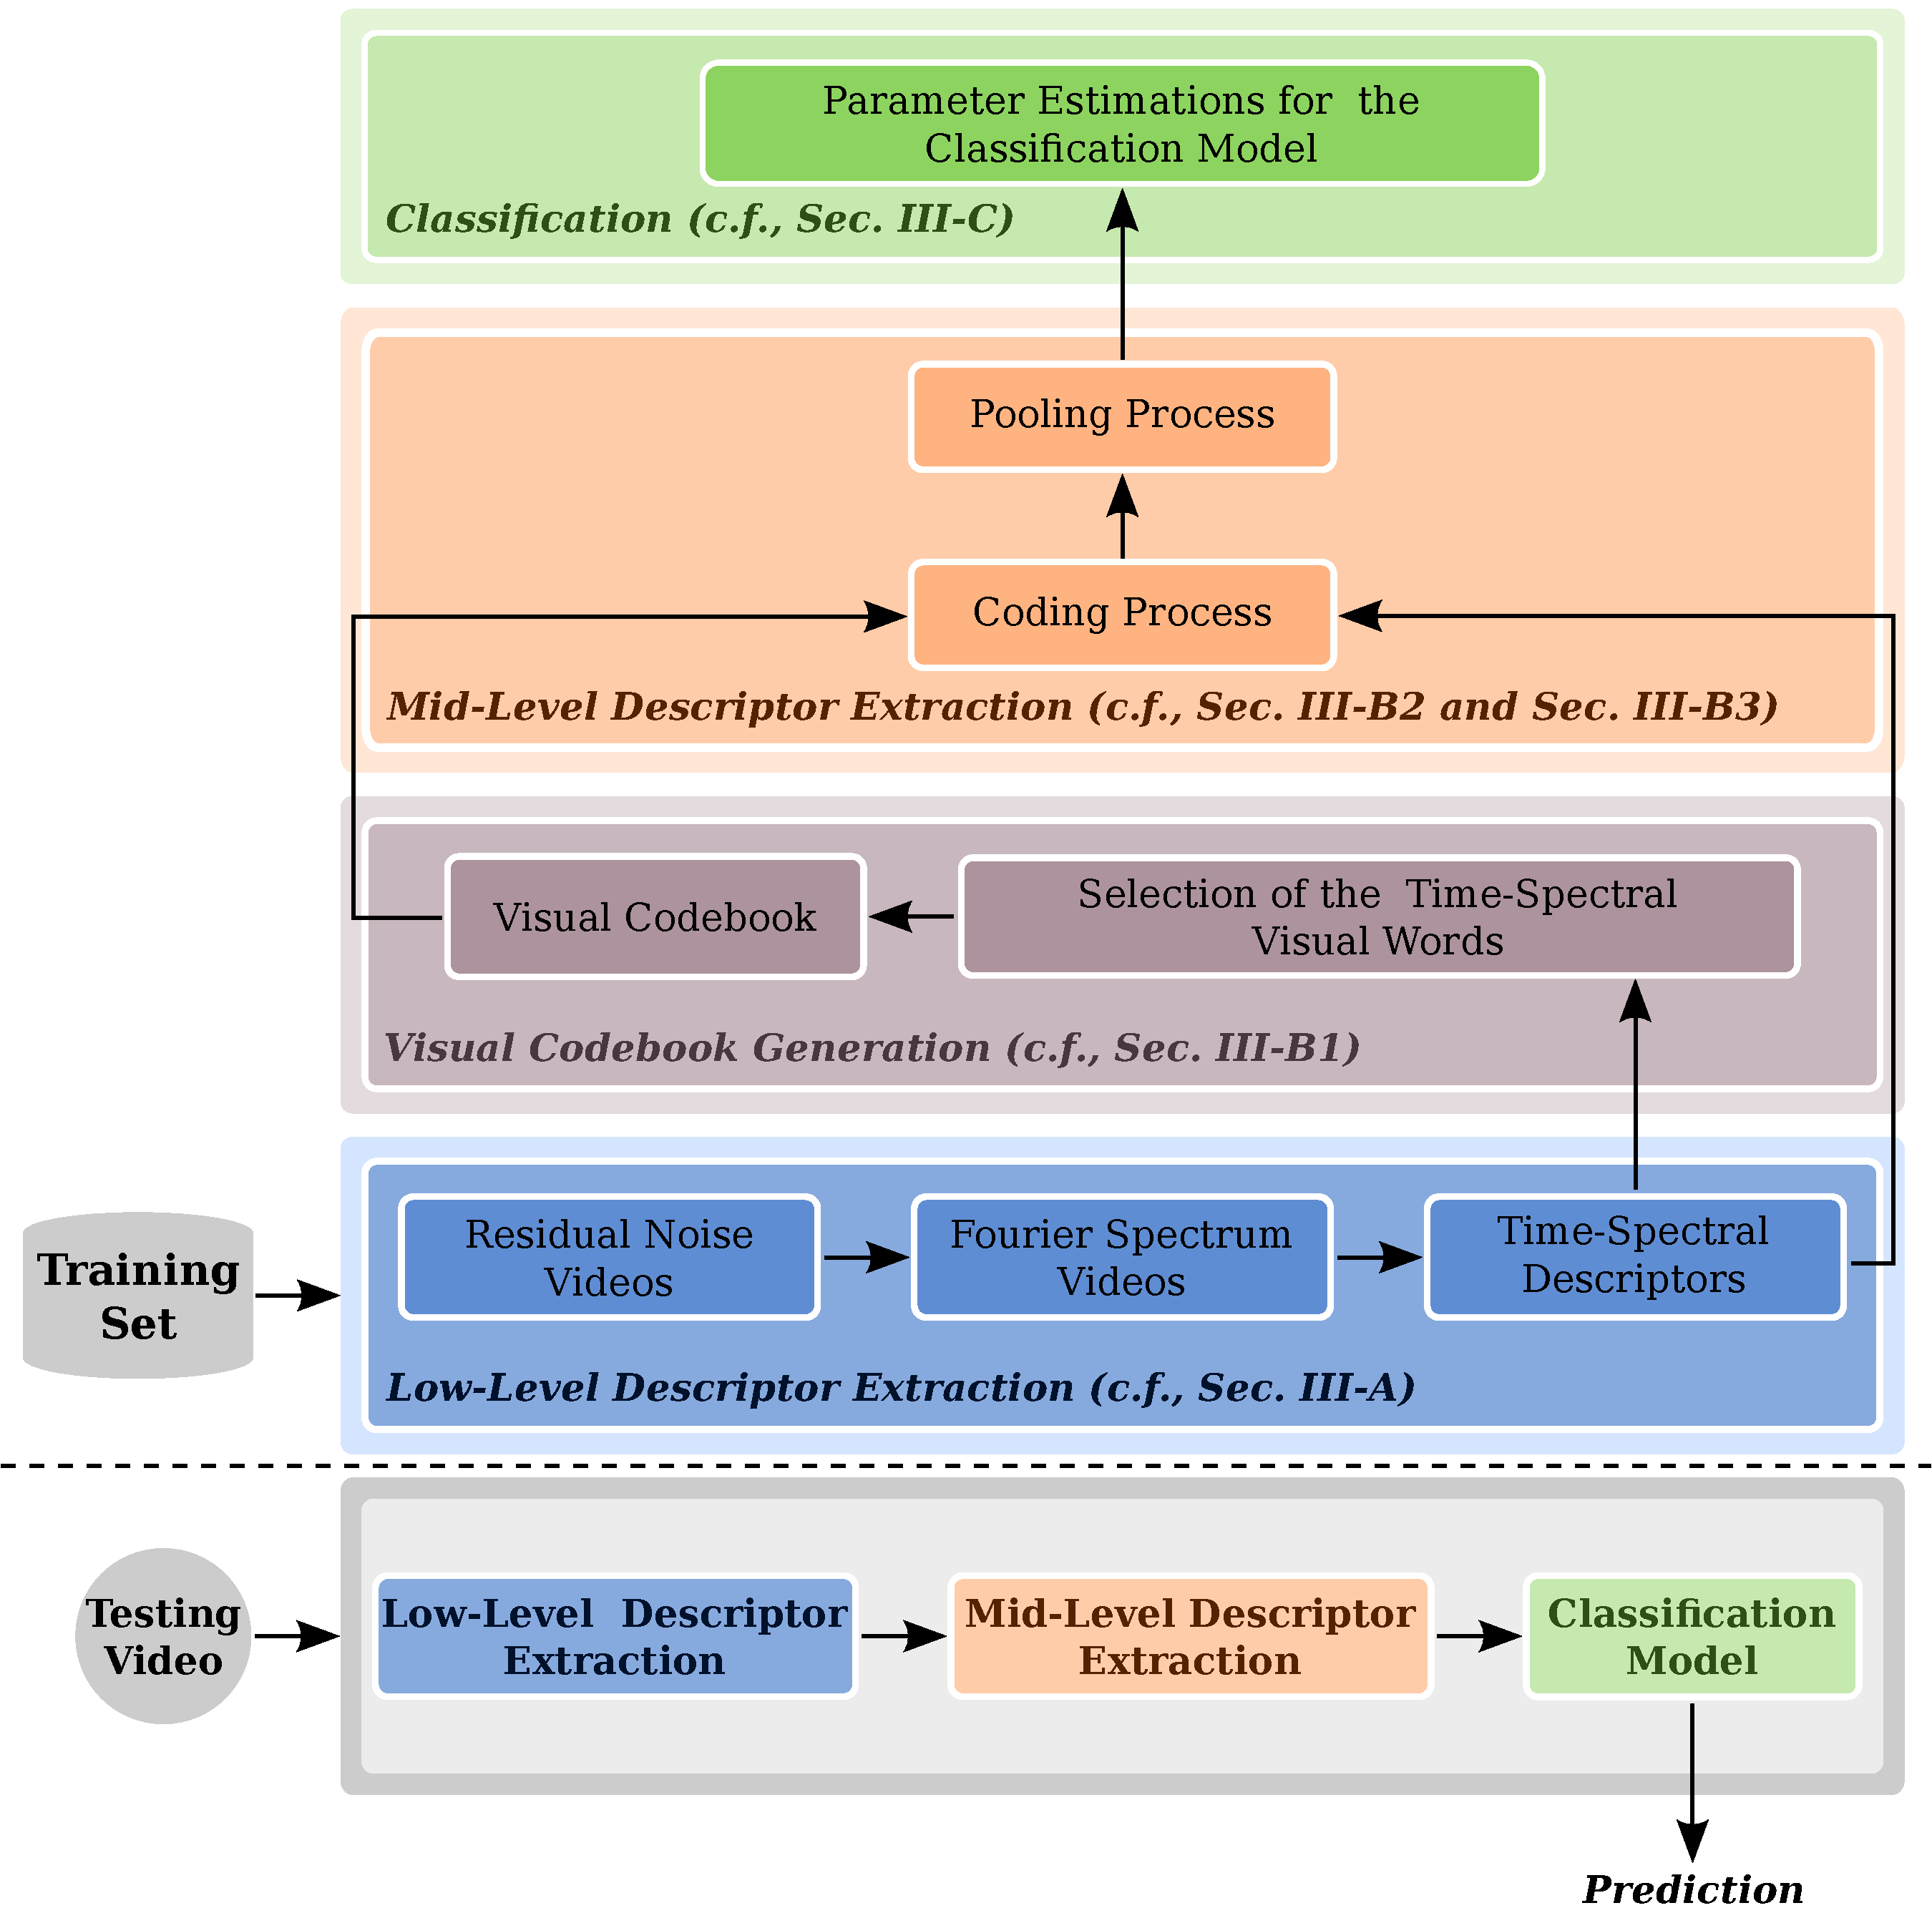
\includegraphics[width=0.45\textwidth]{method_overview_v1.pdf}
\caption{Main steps of the proposed method. Given a training set consisting of valid access and attempted attack videos, and also a testing video, we first extract a noise signature from every training video, generating a \allan{residual noise video}, and calculate its spectrum video. Then, we extract time-spectral descriptors from spectrum videos (low-level representation), which \minor{are used to generate} a visual codebook. With the visual codebook at hand, we transform the low-level descriptors in time-spectral visual word descriptors (mid-level representation). Finally, these mid-level descriptors are used to find parameters of the classification model, which \minor{are employed to predict} whether a given testing video is an attempted attack.}
\label{fig:method_overview}
\end{figure}

\minor{Recent works~\cite{Maatta:IJCB:2011, Pinto:SIBGRAPI:2012, Tan:ECCV:2010} show that noise and artifacts such as blurring effects, printing artifacts, banding effects, and Moir\'{e} patterns are added to the synthetic biometric samples during their manufacture and recapture. In this paper, we propose a spatio-temporal algorithm that captures such effects along time to provide an effective discriminative signature for valid access and spoofing attempts. In summary, the main contributions of this paper are:}
%
\begin{itemize}
	\item a new method for extracting temporal and spectral information from face biometric samples, referred to as time-spectral descriptors;
	\item evaluation of the visual codebook model, also referred to as Bag-of-Visual-Word model, for creating a mid-level representation from time-spectral descriptors, referred to as time-spectral visual words; and
	\item a low-cost solution for spoofing detection, \minor{illustrated in Figure~\ref{fig:method_overview}}, that does not rely on the user interaction or on extra hardware (e.g., infrared, motion or depth sensors) to detect different types of synthetic samples or attacks (e.g., photos, videos and masks) and is amenable to be implemented in computational devices such as PCs, handheld, and embedded systems. 
\end{itemize}

We organize the remaining of this paper as follows. Section~\ref{sec:relatedwork} discusses state-of-the-art methods for face spoofing attack detection. Section~\ref{sec:method} presents our method for spoofing attack detection. Section~\ref{sec:experimentalresults} shows and discusses the experimental protocol and the obtained results. Finally, Section~\ref{sec:conclusions} concludes the paper and discusses possible future work.

%!TEX root = 2014-TIFS-dl-spoofing.tex
\section{Related Work}
\label{sec:relatedwork}
In this section, we review anti-spoofing related work for iris, face, and fingerprints, our focus in this paper.

\subsection{Iris Spoofing}
Daugman~\cite[Section 8 -- Countermeasures against Subterfuge]{Daugman:1999}\footnote{It also appears in a lecture of Daugman at IBC 2004~\cite{ Daugman:IBC:2004}.} was one of the first authors to discuss the feasibility of some attacks on iris recognition systems. The author proposed the use of Fast Fourier Transform to verify the high frequency spectral magnitude in the frequency domain.

%From the analysis of the iris patterns, it is possible to distinguish a printed iris image from a real one due to the characteristics of the periodic dot printing.

The solutions for iris liveness detection available in the literature range from active solutions relying on  special acquisition hardware~\cite{Lee:LNCS:2005,Pacut:2006,Kanematsu:2007} to software-based solutions relying on texture analysis of the  effects of an attacker using color contact lenses with someone else's pattern printed onto them~\cite{Wei:2008}. Software-based solutions have also explored the effects of cosmetic contact lenses~\cite{Kohli:ICB:2013,Doyle:BTAS:2013,Bowyer:Computer:2014,Yadav:TIFS:2014}; pupil constriction~\cite{Huang:WACV:2013}; and multi biometrics of  electroencephalogram (EEG) and iris together~\cite{Kathikeyan:ICCCA:2012}, among others.

%Nonetheless, in the followings of this subsection, we describe in details those works directly related to the databases we use in this article.

%In \cite{Lee:LNCS:2005}, Lee et al. proposed a new method based on the theoretical positions and distances between the Purkinje image (reflections of objects from the structure of the eye) based on the human eye model by using two alternating collimated \emph{Infra-Red Light Emitting Diode} (IR-LED) requiring special hardware and constrained environment. Experiments using 30 persons (10 without glasses and no contact lens, 10 without glasses and using contact lenses, and with glasses and no contact lens) and 15 counterfeit samples (2D printed iris image, 3D artificial eye and 3D patterned contact lens) were acquired. The real and fake samples where evaluated 10 and 20 times each one, respectively. The obtained results showed impressive results: 0.33 (1/300) false acceptance rate (FAR) and false rejection rate (FRR).

%In \cite{Pacut:2006}, Pacut \& Czajka introduced three liveness detection algorithm based on analysis of image frequency spectrum (FS), controlled light reflection (CLR )from the cornea and pupil dynamics (PD). These methodologies were evaluated using printed fake eye images produced with different printers and printout carries. A small hole is made in place of the pupil, and this trick was enough for fake iris capturing by commercial systems. The experimental results obtained on the evaluation set composed of only 77 pairs of fake and live iris images showed that the CLR and PD methodologies achieves zero error rates and two commercial cameras have achieved $73.1\%$ and $15.6\%$ of FAR for these fake images.

%Kanematsu et al.~\cite{Kanematsu:2007} have proposed a new method by using a variation in the brightness of an iris pattern induced by a pupillary reflex caused by flash-light illumination, and the classification were performed by a decision threshold of $7\%$ brightness variation rate, which is statistically defined by means of mean and standard variation. Experiments were performed using only 5 images by varying the intensity of illumination in several levels. However no effectiveness rates are reported in this work.

%In \cite{Wei:2008}, Wei et al have addressed the problem of iris liveness detection based on three texture measures: iris edges sharpness (ES), iris-texton feature for characterizing the visual primitives of iris texture (IT) and using selected features based on co-occurrence matrix (CM). In special, they use fake iris wearing color contact lens with textures printed onto them. The experiments showed that the ES feature achieved comparable results to the state-of-the-art methods at that time, and the IT and CM measures outperform the state-of-the-art.

Galbally et al.~\cite{Galbally:ICB:2012} investigated 22 image quality measures (e.g., focus, motion, occlusion, and pupil dilation).
The best features are selected through sequential floating feature selection (SFFS)~\cite{Pudil:PRL:1994} to feed a quadratic discriminant classifier. The authors validated the work on the BioSec~\cite{Fierrez-Aguilar:2007,Ruiz-Albacete:BIOID:2008} benchmark. Sequeira et al.~\cite{Sequeira:VISAPP:2014} 
also explored image quality measures~\cite{Galbally:ICB:2012} and three classification techniques validating the work on the BioSec~\cite{Fierrez-Aguilar:2007,Ruiz-Albacete:BIOID:2008} and Clarkson~\cite{LivDet:Iris:2013} benchmarks and introducing the MobBIOfake benchmark comprising 800 iris images from the MobBIO multimodal database~\cite{Sequeira:VISAPP:2014:base}.

Sequeira et al.~\cite{Sequeira:IJCNN:2014} extended upon previous works also exploring quality measures. They first used a feature selection step on the features of the studied methods to obtain the ``best features'' and then used well-known classifiers for the decision-making. In addition, they applied iris segmentation~\cite{Monteiro:CCIS:2014} to obtaining the iris contour and adapted the feature extraction processes to the resulting non-circular iris regions. The validation considered five datasets (BioSec~\cite{Fierrez-Aguilar:2007,Ruiz-Albacete:BIOID:2008}, MobBIOfake~\cite{Sequeira:VISAPP:2014:base}, Warsaw~\cite{Czajka:MMAR:2013}, Clarkson~\cite{LivDet:Iris:2013} and NotreDame~\cite{Doyle:2014:base}.

Textures have also been explored for iris liveness detection. In the recent MobILive\footnote{MobLive 2014, Intl. Joint Conference on Biometrics (IJCB).}~\cite{Sequeira:IJCB:2014} iris spoofing detection competition, the winning team explored three texture descriptors: Local Phase Quantization (LPQ)~\cite{Ojansivu:ISP:2008}, Binary Gabor Pattern~\cite{Zhang:ICIP:2012}, and Local Binary Pattern (LBP)~\cite{Ojala:TPAMI_2002}.

Analyzing printing regularities left in printed irises, Czajka~\cite{Czajka:MMAR:2013} explored some peaks in the frequency spectrum were associated to spoofing attacks. For validation, the authors introduced the Warsaw dataset containing 729 fake images and 1,274 images of real eyes. 
In~\cite{LivDet:Iris:2013}, The First Intl. Iris Liveness Competition in 2013, the Warsaw database was also evaluated, however, the best reported result achieved $11.95\%$ of FRR and $5.25\%$ of FAR by the University of Porto team.

%For localizing the peaks, the author sets up two disjoint frequency windows located under the iris. The window is used to observe the artifacts inserted during printing processing and the second window serves as a reference to the observed disturbances in an amplitude spectrum. Finally, a liveness score is calculated based on information from these two windows. In this dataset, it is claimed that the methodology can be set up to obtain no false alarms ($0\%$ of false rejection rate (FRR)) and $5\%$ of false acceptance rate (FAR). 

%Although not directly related to the datasets in our work, it is worthwhile to describe a recent work of 

Sun et al.~\cite{Sun:TPAMI:2014} recently proposed a general framework for iris image classification based on a Hierarchical Visual Codebook (HVC). The HVC encodes the texture primitives of iris images and is based on two existing bag-of-words models. The method achieved state-of-the-art performance for iris spoofing detection, among other tasks.

%Moreover, the authors also developed an iris image dataset with four types of fake iris patterns (iris texture printed on paper, plastic eyeballs, contact lens and synthetic fake iris images) called CASIA-Iris-Fake. The authros claimed that it is the first dataset comprising a large variety of fake iris patterns allowing an advance on the development of unified countermeasures against spoofing attacks. 

In summary, iris anti-spoofing methods have explored hard-coded features through image-quality metrics, texture patterns, bags-of-visual-words and noise artifacts due to the recapturing process. The performance of such solutions vary significantly from dataset to dataset. Differently, here we propose the automatically extract vision meaningful features directly from the data using deep representations.


\subsection{Face Spoofing}
%Spoofing attack is easily performed against face biometrics systems due to low cost to produce a fake sample. As a matter of fact, there are excellent quality printers and digital cameras at a low price nowadays. In addition, the ease in obtaining facial information of a person through social networks and personal pages contributes for low-cost high-profit attacks.

We can categorize the face anti-spoofing methods into four groups~\cite{Schwartz:IJCB:2011}: user behavior modeling, methods relying on extra devices~\cite{Yi:2014}, methods relying on user cooperation and, finally, data-driven characterization methods. In this section, we review data-driven characterization methods proposed in literature, the focus of our work herein.

M\"{a}\"{a}tt\"{a} et al.~\cite{Maatta:IJCB:2011} used LBP operator for capturing printing artifacts and micro-texture patterns added in the fake biometric samples during acquisition. Schwartz et al.~\cite{Schwartz:IJCB:2011} explored color, texture, and shape of the face region and used them with Partial Least Square (PLS) classifier for deciding whether a biometric sample is fake or not. Both works validated the methods with the Print Attack benchmark~\cite{Anjos:IJCB:2011}. Lee et al.~\cite{Lee:ICASSP:2013} also explored image-based attacks and proposed the frequency entropy analysis for spoofing detection.

%Results of these two techniques were reported in the Competition on Counter Measures to 2D Facial Spoofing Attacks~\cite{Chakka:IJCB:2011}, with a Half Total Error Rate (HTER) of $0.00\%$ and $0.63\%$, respectively, upon the Print Attack database~\cite{Anjos:IJCB:2011}.

% as space is required and this approach does not improved the previously existing one, it was removed
%Inspired on the work of M\"{a}\"{a}tt\"{a} et al.~\cite{Maatta:IJCB:2011}, Chingovska et al.~\cite{Chingovska:BIOSEG:2012} investigated the use of different variations of the LBP method, such as LBP$^{u2}_{3 \times 3}$, tLBP (transitional), dLBP (direction-coded) and mLBP (modified LBP). The feature vectors obtained with these descriptors were classified through $\chi^{2}$ histogram comparison, linear discriminant analysis (LDA) and SVM. However, the method did not outperform the original one~\cite{Maatta:IJCB:2011}. 

Pinto et al.~\cite{Pinto:SIBGRAPI:2012} pioneered research on video-based face spoofing detection. They proposed visual rhythm analysis to capture temporal information on face spoofing attacks.

%Firstly, the face region is isolated and normalized using $z$-score. Thereafter, independent component analysis (ICA) is used to eliminate cross-channel noise caused by interference from the environment. Finally, the authors use the power spectrum and analyze the entropy of the RBG channels individually to further decide upon the attack based on an empirical threshold.

%During a video-based spoofing attack, a noise signature is added to the biometric samples during the recapture of the attack videos and can be used successfully to detect such attacks.

Mask-based face spoofing attacks have also been considered thus far. Erdogmus et al.~\cite{Erdogmus:BIOSIG:2013} dealt with the problem through Gabor wavelets: local Gabor binary pattern histogram sequences~\cite{Zhang:ICCV:2005} and Gabor graphs~\cite{Wiskott:TPAMI:1997} with a Gabor-phase based similarity measure~\cite{Gunther:ICANN:2012}. Erdogmus \& Marcel~\cite{Erdogmus:BTAS:2013} introduced the 3D Mask Attack database (3DMAD), a public available 3D spoofing database, recorded with Microsoft Kinect sensor.

%They also investigate the use of the LBP-based method and reported an HTER of $0.95\%$ and $1.27\%$ using the color and depth images, respectively.

Kose et al.~\cite{Kose:ICASSP:2013} demonstrated that a face verification system is vulnerable to mask-based attacks and, in another work, Kose et al.~\cite{Kose:FG:2013} evaluated the anti-spoofing method proposed by M\"{a}\"{a}tt\"{a} et al.~\cite{Maatta:IJCB:2011} (originally proposed to detect photo-based spoofing attacks). 
Inspired by the work of Tan et al.~\cite{Tan:ECCV:2010}, Kose et al.~\cite{Kose:DSP:2013} evaluated a solution based on reflectance to detect attacks performed with 3D masks. 

%The authors reported an Area Under the Curve (AUC) of $97.0\%$ and a classification accuracy of $94.47\%$ using the non-public available MORPHO database~\cite{Kose:FG:2013}.

Finally, Pereira et al.~\cite{Pereira:ICB:2013} proposed a score-level fusion strategy in order to detect various types of attacks. 
%The authors trained classifiers using different databases and used the $Q$ statistic to evaluate the dependency between classifiers.
%The combination of classifiers that are statistically independent leads to better results. 
In a follow-up work, Pereira et al.~\cite{Pereira:JIVP:2014} proposed an anti-spoofing solution based on the dynamic texture, a spatio-temporal version of the original LBP. Results showed that LBP-based dynamic texture description has a higher effectiveness than the original LBP.

In summary, similarly to iris spoofing detection methods, the available solutions in the literature mostly deal with the face spoofing detection problem through texture patterns (e.g., LBP-like detectors), acquisition telltales (noise), and image quality metrics. Here, we approach the proplem by extracting meaningful features directly from the data regardless of the input type (image, video, or 3D masks).


\subsection{Fingerprint Spoofing}
%There are several approaches for fingerprint spoofing detection. 
We can categorize fingerprint spoofing detection methods roughly into two groups: hardware-based (exploring extra sensors) and software-based solutions (relying only on the information acquired by the standard acquisition sensor of the authentication system)~\cite{Ghiani:ICB:2013}. 

%Methods following the first approach use information provided from additional sensors to gather artifacts that reveal a spoofing attack that are outside of the fingerprint image. Software-based techniques rely only on the information acquired by the standard acquisition sensor of the authentication system.

Galbally et al.~\cite{Galbally:BIDS:2009} proposed a set of feature for fingerprint liveness detection based on quality measures such as ridge strength or directionality, ridge continuity, ridge clarity, and integrity of the ridge-valley structure. The validation considered the three benchmarks used in LivDet 2009 -- Fingerprint competition~\cite{Marcialis:ICIAP:2009} captured with different optical sensors: Biometrika, CrossMatch, and Identix. Later work~\cite{Galbally:FGCS:2012} explored the method in the presence of gummy fingers.

%The authors built a Biometrika.ATVS  set using the Biometrika database from LivDet 2009 -- Fingerprint competition, and obtained results showing that user cooperation may hinder spoofing attacks.}

%The authors reported an average error of $1.83\%$, $11.12\%$, and $6.73\%$ using Biometrika, CrossMatch and Identix sets, respectively. 


Ghiani et al.~\cite{Ghiani:ICPR:2012} explored LPQ~\cite{Ojansivu:ISP:2008}, a method for representing all spectrum characteristics in a compact feature representation form. The validation considered the four benchmarks used in the LivDet 2011 -- Fingerprint competition~\cite{Yambay:ICB:2012}.

%The authors proposed a rotation-invariant version of LPQ, referenced as Rotation Invariant Local Phase Quantization (RILPQ). 

%A combination between proposed LPQ and LBP yielded even better results with a misclassification rate of $9.2\%$ considering the LivDet 2011 -- Fingerprint competition sets.

Gragnaniello et al.~\cite{Gragnaniello:BIOMS:2013} explored the Weber Local Image Descriptor (WLD) for liveness detection, well suited to high-contrast patterns such as the ridges and valleys of fingerprints images. In addition, WLD is robust to noise and illumination changes. The validation considered the LivDet 2009 and LivDet 2011 -- Fingerprint competition datasets.

%The misclassification rates reported were $7.13\%$ and $27.67\%$, respectively. When the proposed method is combined with RILPQ~\cite{Ojansivu:ICPR:2008}, the misclassification rates in both sets reduce to $3.13\%$ and $12.65\%$, respectively.

Jia et al.~\cite{Jia:ICB:2013} proposed a liveness detection scheme based on Multi-scale Block Local Ternary Patterns (MBLTP). 
Differently of the LBP, the Local Ternary Pattern operation is done on the average value of the block instead of the pixels being more robust to noise. 
The validation considered the LivDet 2011 -- Fingerprint competition benchmarks.

Ghiani et al.~\cite{Ghiani:BTAS:2013} explored Binarized Statistical Image Features (BSIF) originally proposed by Kannala et al.~\cite{Kannala:ICPR:2012}. The BSIF was inspired in the LBP and LPQ methods. In contrast to LBP and LPQ approaches, BSIF learns a filter set by using statistics of natural images~\cite{Hyvrinen:NIS:2009}. The validation considered the LivDet 2011 -- Fingerprint competition benchmarks.

Recent results reported in the LivDet 2013 Fingerprint Liveness Detection Competition~\cite{Ghiani:BTAS:2013} show that fingerprint spoofing attack detection task is still an open problem with results still far from a perfect classification rate.

We notice that most of the groups approach the problem with hard-coded features sometimes exploring quality metrics related to the modality (e.g., directionality and ridge strength), general texture patterns (e.g., LBP-, MBLTP-, and LPQ-based methods), and filter learning through natural image statistics. This last approach seems to open a new research trend, which seeks to model the problem learning features directly from the data. We follow this approach in this work, assuming little a priori knowledge about acquisition-level biometric spoofing and exploring deep representations of the data.


%The best classification results among four used datasets were achieved by one team of the University of Naples Federico II and another from the Dermalog Identification Systems. They reported an average accuracy of $86.63\%$ and $84.63\%$, respectively.

\subsection{Multi-modalities}

Recently, Galbally et al.~\cite{Galbally:TIP:2014} proposed a general approach based on 25 image quality features to detect spoofing attempts in face, iris, and fingerprint biometric systems. Our work is similar to theirs in goals, but radically different with respect to the methods.
Instead of relying on prescribed image quality features, we build features that would be hardly thought by a human expert with AO and FO.
Moreover, here we evaluate our systems in more recent and updated benchmarks.


% done! só deixei in [xx] quando era referenciada uma competição.
%\TODO{Algumas vezes usa in [xx] e outras author at al.[xx], acho que poderia padronizar para author et al.[xx], quando possível, por exemplo alguns paragrafos sobre finger printe}

\section{Proposed Method}\label{sec:method}
In this section, we introduce a method for detecting different forms of face spoofing attacks. The method comprises three main steps: \emph{low-level descriptor extraction}, \emph{mid-level descriptor extraction}, and \emph{classification}. Fig.~\ref{fig:method_overview} \minor{illustrates} these steps, which we explain in details in the following sections.

We designed the algorithm based on the fact that synthetic biometric samples contain noise and artifacts generated during their manufacture and recapture that are different \minor{from} any pattern found in real biometric samples. According to Tan et al.~\cite{Tan:ECCV:2010} and M\"{a}\"{a}tt\"{a} et al.~\cite{Maatta:IJCB:2011}, there is a deterioration of the facial information and, consequently, a loss of some high frequency components during the manufacture of photographs to be used in spoofing attacks. In our prior work~\cite{Pinto:SIBGRAPI:2012}, we highlighted the fact that there is a significant increase of the low frequency components due to the blurring effect added during the recapture process of the biometric sample displayed in tablets, smartphones and laptop screens. Besides the blurring effect, other artifacts are added \redmark{such as flickering, Moir\'e patterns, and banding effect~\cite{Beach:PP:2008}}.

\redmark{These facts motivated us to propose a solution that takes advantage of the noise and artifacts contained on such fake biometric samples, which heretofore we refer to as a noise signature. We perform a Fourier analysis of the noise signature to capture the information encoded in the frequency, phase and amplitude of the component sinusoids~\cite{Smith:SEG:1997}. In this paper, we use Fourier spectrum to quantify the following artifacts:}
%
\begin{itemize}
	\item \textit{\redmark{blurring artifact}:} In both the production and recapture processes, inevitably we have a decrease in the details of biometric samples due to re-quantization of the original signal. This reduction of details is reflected in the increase of low frequency components and can be observed in the Fourier domain;
	
	\item \textit{flickering effect:} It corresponds to the horizontal and vertical lines equally spaced that appear during the recapture process of the samples shown to the acquisition sensor with the display device. When this artifact appears in biometric samples, there are peak lines at abscissa and ordinate axes of the Fourier spectrum when the display device is aligned with the acquisition sensor;
	
	\item \textit{\redmark{Moir\'e pattern}:} They are irregular patterns \redmark{that can appear} when a display device is used to perform an attempted attack. As a result, we also have the appearance of peaks in different locations in the Fourier spectrum depending on the {frequency and direction of the sinusoid in the spatial domain}~\cite{Smith:SEG:1997}.
\end{itemize}

The novelty of our solution is in the two-tier low and mid-level characterization scheme, called time-spectral visual words, that captures patterns present in such noise signatures useful to reveal spoofing attacks. For this, we extract \redmark{temporal-spectral descriptors} from the noise signature transformed to the frequency domain and create a mid-level representation for them using the concept of visual codebooks~\cite{Sivic:ICCV:2003,Avila:ICIP:2011}. Visual codebooks are a method for constructing mid-level representations widely employed in several applications in pattern recognition and computer vision, \allan{such as object recognition~\cite{Vigo:ICPR:2010}, gesture recognition~\cite{Vela:ICPR:2012}, and information retrieval~\cite{Penatti:PR:2014}, among others}. However, \minor{unlike existing methods, we obtain visual informative features} from the \redmark{noise signature present in the videos} instead of their raw pixels or from objects in the scene. 

\subsection{Low-Level Descriptor Extraction}
In our previous work~\cite{Pinto:SIBGRAPI:2012}, we found that the noise signal is an important source for low-level discriminative features for spoofing detection. When working with the noise signal and discarding the video content, \redmark{we minimize possible negative impacts on the \allan{method performance}. Next, we present the \allan{steps} of the proposed method to compute the low-level descriptors.} 

%\todo{me parece forte falar que a remocao do conteudo reduz o impacto da iluminacao, uma vez que a iluminacao impacta as frequencias espaciais da imagem, talvez tirar a parte do such as e deixar geral para evitar algum comentario do revisor}

\subsubsection{Calculation of the Residual Noise Videos}
The low-level representation of the videos is computed through the spectrum analysis of the noise signal in the frequency domain. To isolate the noise signal of a given video $V$, we filter a copy of $V$ using a Gaussian filter with mean $\mu$, std. $\sigma$, and kernel size $k \times k$ to remove the high frequency components, generating a filtered video. Then, we perform a subtraction operation between the input video and its filtered version, generating a new video, called \redmark{Residual Noise Video ($V_{RN}$)}: 
\begin{equation}
V_{RN}^{(t)} = V^{(t)} - h(V^{(t)}) \quad \forall \textrm{ \textit{t} } \in \mathit{T} =\{1, 2, \ldots, t\},
\label{eq:ruido}
\end{equation}
\noindent where $V^{(t)} \in \mathbb{N}^2$ is the $t$-th frame of $V$ and $h$ is a filter whose impulse response is a Gaussian function.

\subsubsection{Calculation of the Fourier Spectrum Videos}
After calculating the residual noise videos, we can analyze the noise pattern and possible artifacts contained in the biometric samples by applying the 2D Discrete Fourier Transform to each frame of the \allan{$V_{\text{RN}}$} using Eq.~\ref{eq:dft}. In this work, we evaluate two important characteristics of the noise signal in the frequency domain, the magnitude and phase of the signal. The analysis of these two characteristics is performed by calculating the magnitude spectrum (Eq.~\ref{eq:mag_spectrum}) and phase spectrum (Eq.~\ref{eq:phase_spectrum}), with the origin at the center of the frame. In both cases, the result is a Fourier spectrum video.

\begin{small}
\begin{align}
\mathcal{F}{(V_{\text{RN}}(x,y))} &\equiv F(v, u) \\
F(v, u) &= \sum_{x=0}^{M-1}{\sum_{y=0}^{N-1}{V_{\text{RN}}(x,y)e^{-j2\pi[(vx/M) + (uy/N)]}}} \label{eq:dft} \\
|{F}{(v, u)}| &= \sqrt{\mathcal{R}{(v, u)}^{2} + \mathcal{I}{(v, u)}^{2}} \\
V_{\text{MS}}{(v, u)} &= \log(1 + |{F}{(v, u)}|) \label{eq:mag_spectrum} \\
V_{\text{PS}}(v, u) &= \arctan{\left(\frac{\mathcal{I}{(v, u)}}{\mathcal{R}{(v, u)}}\right)} \label{eq:phase_spectrum}
\end{align}
\end{small}

From the Fourier spectrum video, we can extract spectral and temporal information relevant to the spoofing attack detection. In the case of the spectral information, we need to capture peaks present in the central region caused by artifacts that reduce some details in the scene (e.g., skin marking, edge information) such as blurring effect, defocus, and printing artifacts and peaks present in the peripheral region of the frame caused mainly by artifacts such as the banding effect and Moir\'e pattern, which appear during the recapture of the biometric information during an attack. 

\redmark{Figs.~\ref{fig:noise_spectra_real1} and~\ref{fig:noise_spectra_attack1} show an attempt to depict the temporal disturbances added to the biometric samples during attacks. In this example,  we extract the first ten consecutive frames of an attack video and of a valid video for the same client, and calculate their respective magnitudes spectra from the residual noise video. In addition, Fig.~\ref{fig:noise_spectra_attack2} shows examples in which we have frames extracted from valid access videos (a) and spoof attack videos (b-c). In this figure, we aim at showing the Moiré and blurring effects found in attempted attacks performed with a mobile device. The blurring effect is present in the magnitude spectrum with an increase of the low frequency components, whereas the Moiré effect is present in the magnitude spectrum with peaks in the horizontal center region of the frames. It is hard to find a direct mapping of the effects to the phase spectra, but we can see clearly that there are disturbances in the phase spectra calculated from attempted attack frames when compared to phase spectra extracted from valid access frames.}

\minor{It is important to remark that} we are not proposing a method \minor{for capturing} each of the artifacts separately. We believe that the presence of one or more artifacts \minor{causes} disturbances in the frequency components in the Fourier domain and the proposed method aims at describing and capturing this disturbance in space and time.
%
\begin{figure*}[!htb]
	\centering
	\subfloat[Original frames]{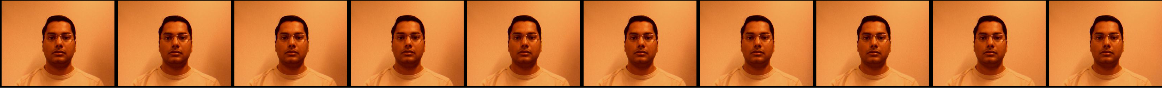
\includegraphics[width=0.75\textwidth]{./original_train/real/client004_session01_webcam_authenticate_controlled_1.png}}\\
	\subfloat[Residual noise frames]{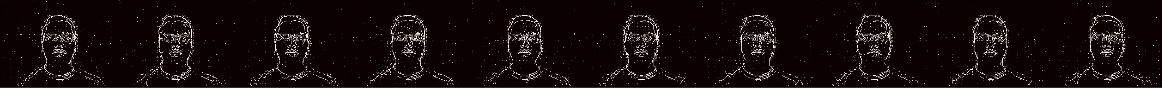
\includegraphics[width=0.75\textwidth]{./ritmo_noisetrain/real/client004_session01_webcam_authenticate_controlled_1.png}}\\
	\subfloat[Magnitude spectra]{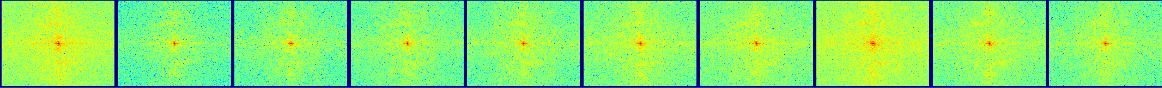
\includegraphics[width=0.75\textwidth]{./ritmo_spectrain/real/client004_session01_webcam_authenticate_controlled_1.png}}
	\caption{(a) Original frames extracted from a valid access video, (b) their respective \allan{residual noise frames} and (c) magnitude spectra.
	\label{fig:noise_spectra_real1}}
\end{figure*}
%
\begin{figure*}[htb]
	\centering
	\subfloat[Original frames]{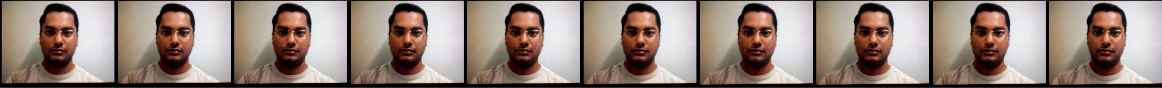
\includegraphics[width=0.75\textwidth]{./original_train/attack/hand/attack_mobile_client004_session01_mobile_photo_controlled.png}}\\
	\subfloat[Residual noise frames]{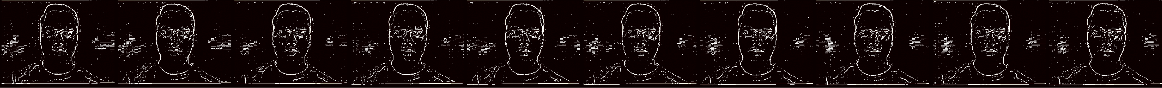
\includegraphics[width=0.75\textwidth]{./ritmo_noisetrain/attack/hand/attack_mobile_client004_session01_mobile_photo_controlled.png}}\\
	\subfloat[Magnitude spectra]{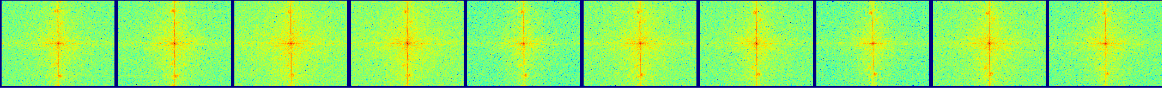
\includegraphics[width=0.75\textwidth]{./ritmo_spectrain/attack/hand/attack_mobile_client004_session01_mobile_photo_controlled.png}}
	\caption{(a) Original frames extracted from an attempted attack video, (b) their respective \allan{residual noise frames} and (c) magnitude spectra.
	\label{fig:noise_spectra_attack1}}
\end{figure*}
%
\begin{figure*}[!htp]
	\centering
	\subfloat[Examples of a frame extracted from valid access video]{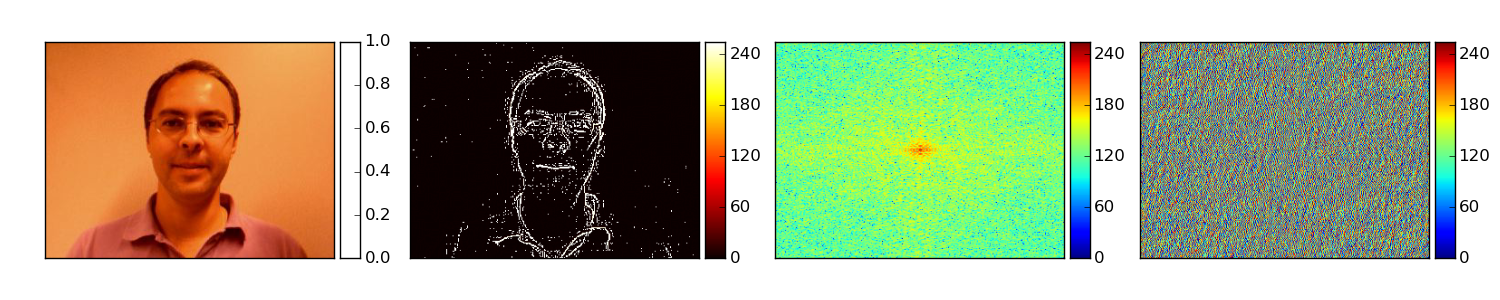
\includegraphics[width=0.68\textwidth]{client001_session01_webcam_authenticate_controlled_1_000.png}}\\
	\subfloat[Examples of frames extracted from a mobile-attack videos. We highlighted the Moiré effect with yellow circle in the original image and its respective residual noise frame. The arrows on the magnitude spectrum indicate the effect of the Moiré effect over Fourier spectrum]{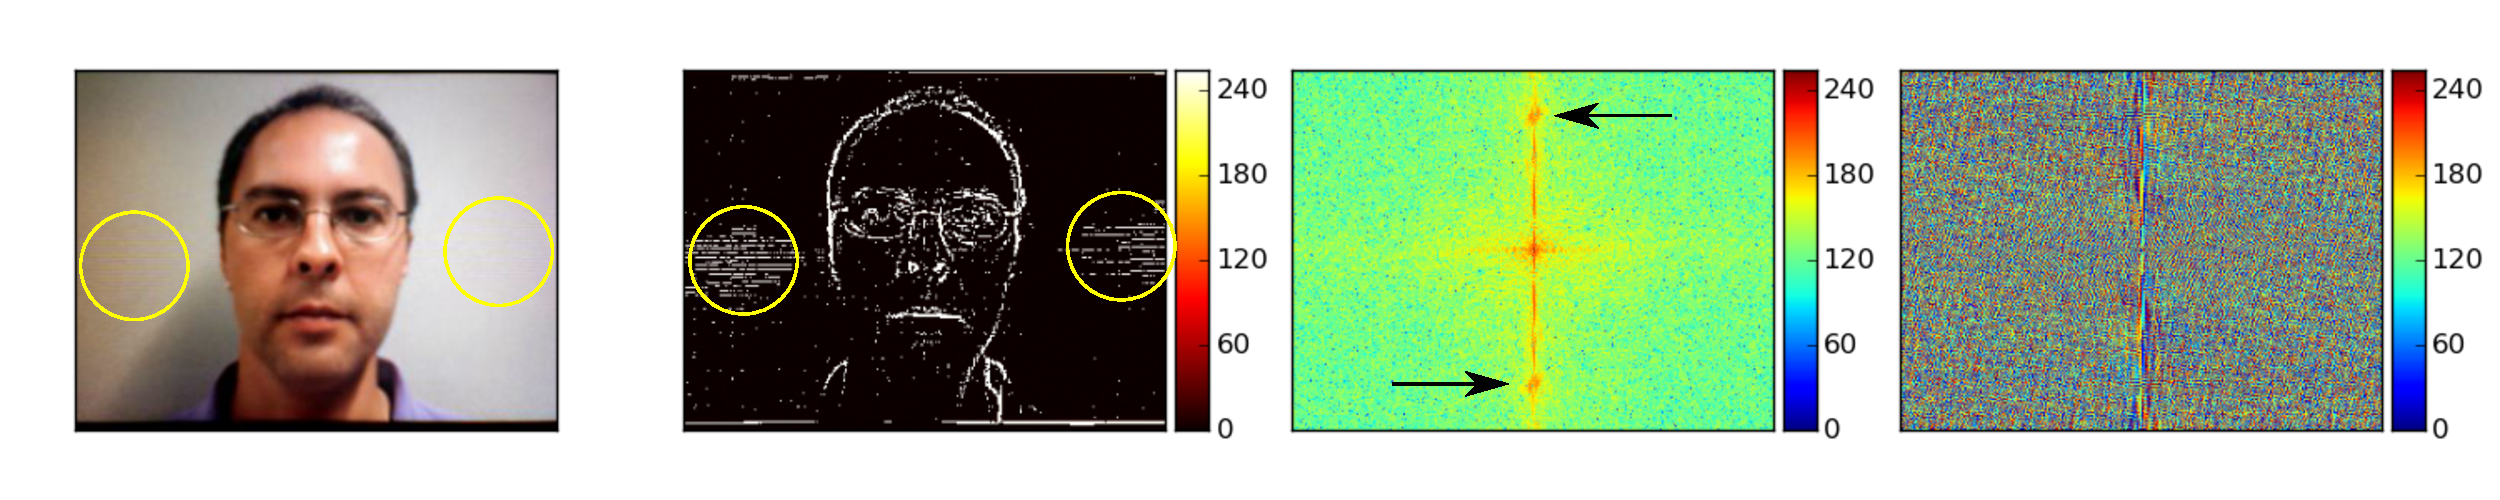
\includegraphics[width=0.68\textwidth]{attack_mobile_client001_session01_mobile_photo_controlled_000.pdf}}\\
	\subfloat[Examples of frames extracted from a mobile-attack videos. In this frame, we show a blurring effect in the original image and its effect in the residual noise frame. The arrows on the magnitude spectrum show the impact of this effect over Fourier spectrum]{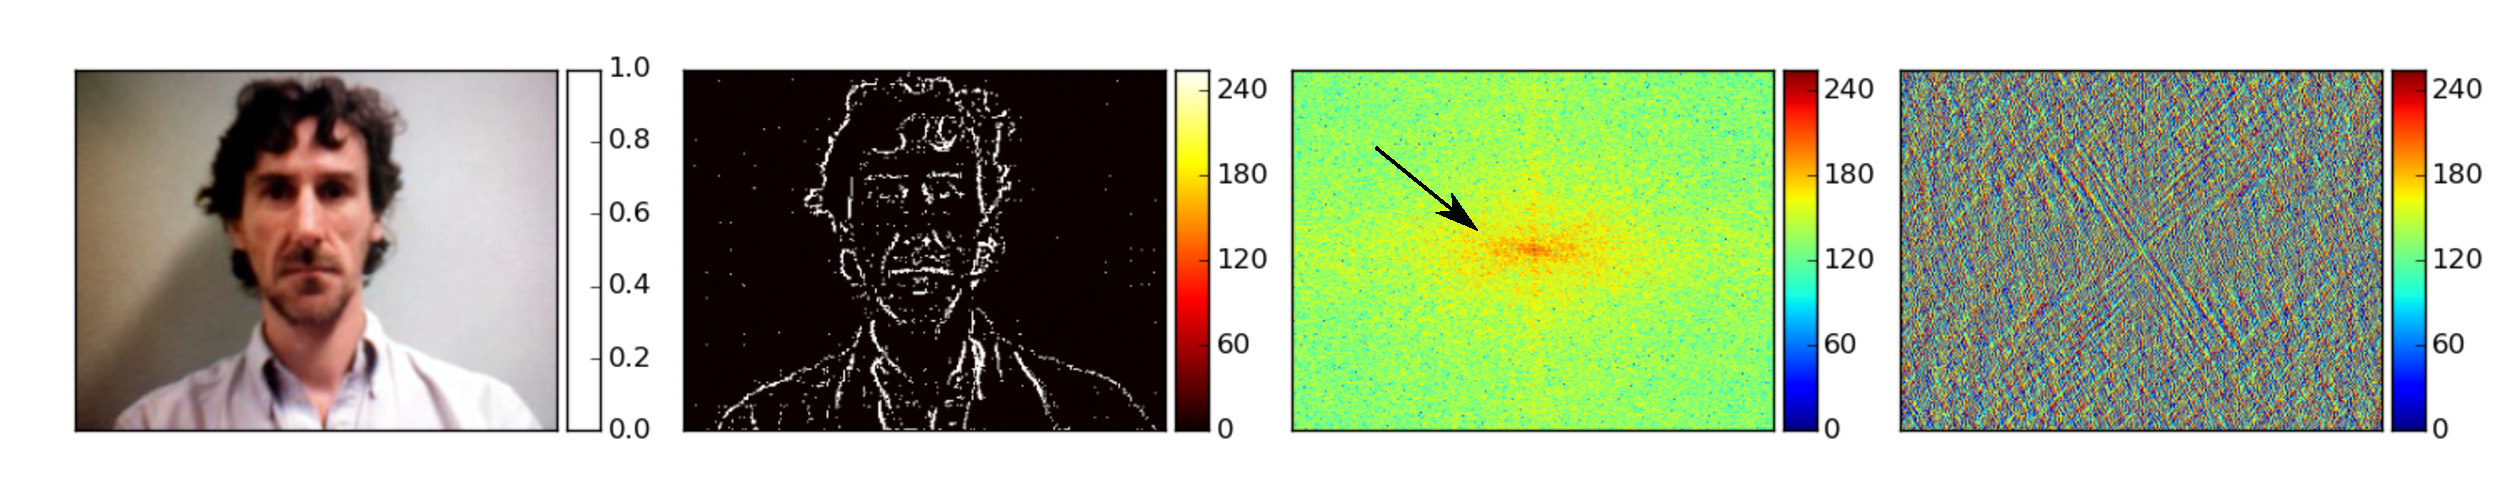
\includegraphics[width=0.68\textwidth]{attack_mobile_client011_session01_mobile_photo_controlled_009.pdf}}\\
	\caption{Examples of valid access and attempted attack videos. The first column shows the original frame extracted from a video and the second column shows the \allan{residual noise frame} calculated from the original frames. Finally, the third and fourth columns show the magnitude and phase spectrum, respectively. Note that the phase spectra calculated from valid access frames are different from attempted attack frames.\label{fig:effects}}
	\label{fig:noise_spectra_attack2}
\end{figure*}
%
%%
%\begin{figure*}[!ht]
%\centering
%\subfloat[Magnitude spectra calculated from a valid access video.]{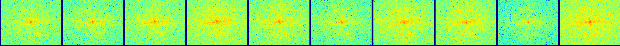
\includegraphics[width=0.82\textwidth]{./figures/temporal/client020_session01_webcam_authenticate_controlled_2.png}}\hspace{1.0mm}
%%
%\subfloat[Magnitude spectra calculated from a spoof attack video.]{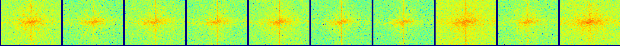
\includegraphics[width=0.82\textwidth]{./figures/temporal/attack_mobile_client020_session01_mobile_video_controlled.png}}
%\caption{Examples of the first ten magnitude spectra calculated from a \textbf{valid access} video (a) and a \textbf{spoof attack} video (b).}
%\label{fig:tempartifacts}
%\end{figure*}
%%
%\begin{figure*}[!ht]
%\centering
%\subfloat[Examples of frames extracted from valid access videos for two users on Replay-Attack dataset.]{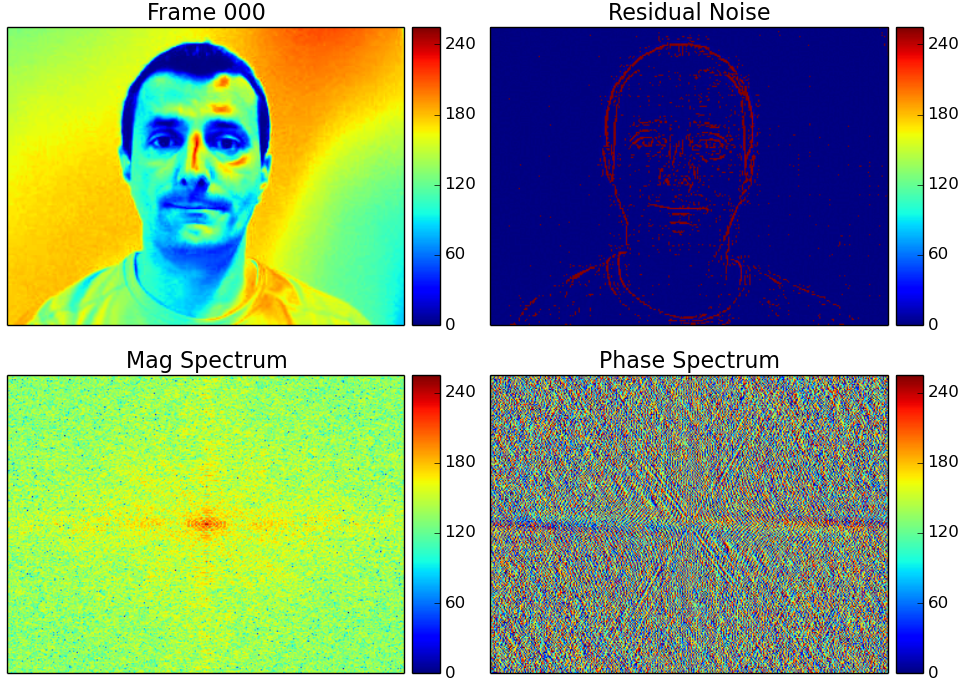
\includegraphics[width=0.39\textwidth]{./figures/artifacts/client026_session01_webcam_authenticate_controlled_1_000.png}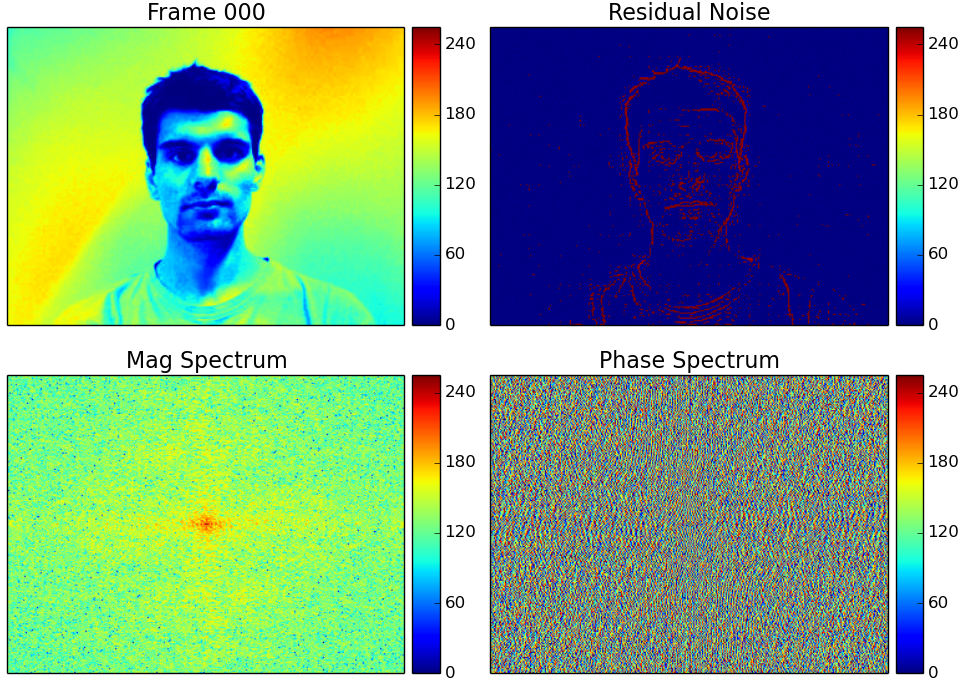
\includegraphics[width=0.39\textwidth]{./figures/artifacts/client020_session01_webcam_authenticate_controlled_1_000.png}}\\
%%
%\subfloat[Example of frame extracted from a spoof attack video.]{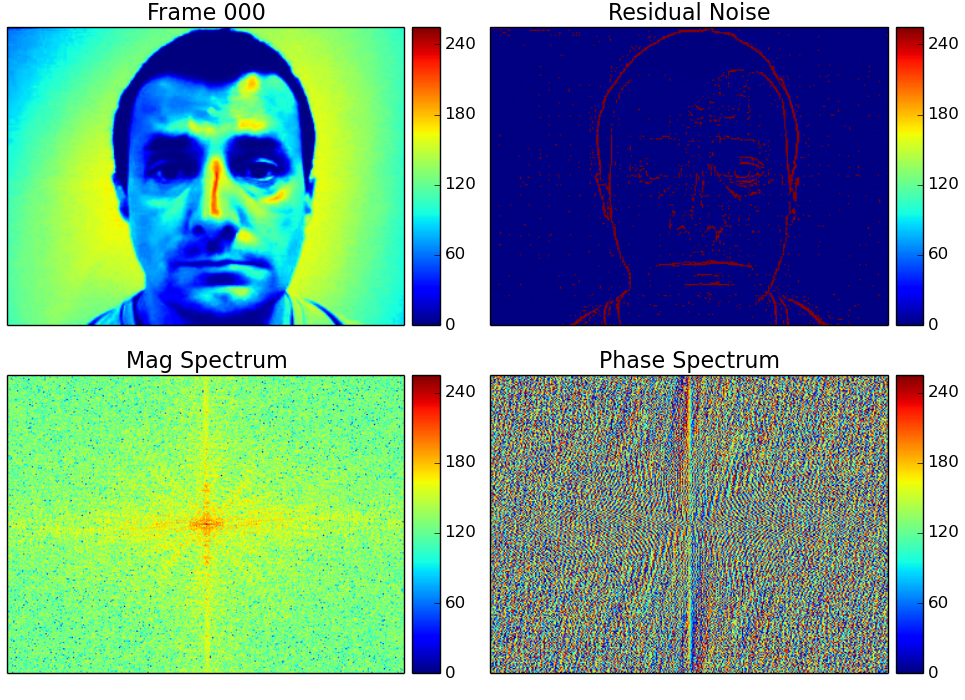
\includegraphics[width=0.39\textwidth]{./figures/artifacts/attack_highdef_client026_session01_highdef_video_controlled_000.png}}\hspace{0.5mm}
%\subfloat[Example of frame extracted from a spoof attack video.]{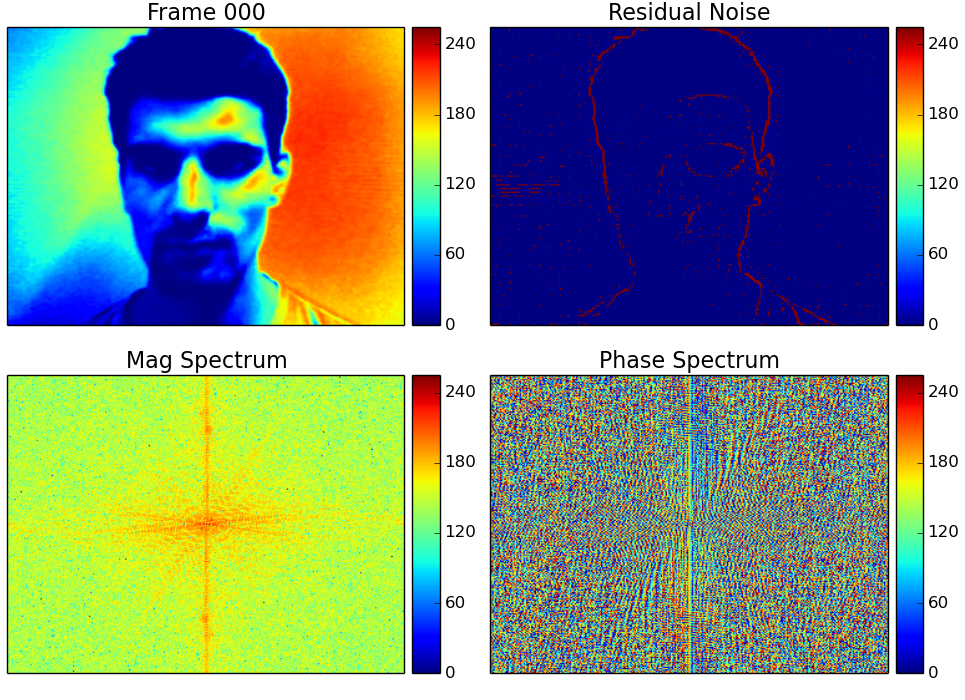
\includegraphics[width=0.39\textwidth]{./figures/artifacts/attack_mobile_client020_session01_mobile_video_controlled_000.png}}
%\caption{Examples of video frames of \textbf{valid access} videos (a) and \textbf{spoof attack} videos (b-c). Fig.\ref{fig:artifacts}(c)~and~(d) illustrate examples of blurring effect, characterized by the loss of details in the face region  and Fig.\ref{fig:artifacts}(b)~and~(c) show flickering effects, characterized by the appearance of collinear points (b) and horizontal traces (c), both in the background.}
%\label{fig:artifacts}
%\end{figure*}

\subsubsection{Computation of the time-spectral descriptor}
Due to the dynamics involved in the appearance of artifacts and noise in the synthetic biometric samples \minor{and the} spectral information, the temporal information becomes important to detect spoofing attacks. Therefore, we design a feature descriptor that gathers temporal and spectral information from an input video. We extract $n$ temporal cubes of size of $w \times h \times t$ \minor{(blocks of size $w \times h$ of $t$ frames) from the Fourier spectrum video}. The idea of temporal cubes has been somewhat explored to quantify temporal information in other tasks in computer vision~\cite{Klaeser:BMVA:2008,Alon:TPAMI:2009,Ren:PR:2009}. In all cases, it always boils down to designing important discriminative features for capturing the event of interest. In this paper, we design new ideas for spoofing detection.

%The extracted temporal cubes are hereinafter named as time-spectral features, which contain information about the temporal behavior of the frequency components that form the input video. 

\minor{The computation of the measure over temporal cubes can be performed on each frame separately, hereinafter referred to as spatial measures, or between consecutive frames, hereinafter referred to spatio-temporal measures. Examples of spatial measures that can be used are energy and entropy of the signal, which quantify the signal size and amount of information, respectively. As examples of spatial-temporal measures, we can mention correlation and mutual information, which are applied to measure dependence between consecutive frames. At the end of this process, we have a set of $n$ time-spectral descriptors of $t$ dimensions, for each video. As spatio-temporal measures are applied on consecutive frames, this process yield $n$ time-spectral descriptors of $(t-1)$ dimensions each.}

\subsection{Mid-Level Descriptor Extraction}
To find a robust representation for the low-level feature descriptors, with less sensitivity to the intra- and extra-class variations, we use the Bag-of-Visual-Word (BoVW) model~\cite{Sivic:ICCV:2003}, which maps the low-level features onto a more discriminative mid-level representation. Methods based on the BoVW model can be understood in the following steps: \minor{visual} codebook generation, coding, and pooling.

\subsubsection{Visual Codebook Generation}
The generation of the visual codebook consists in the selection of time-spectral descriptors that are more frequent and representative considering all descriptors extracted from training videos. The selected descriptors, called time-spectral visual words, form the visual codebook. The selection can be performed using two strategies: (1) random selection, whereby all descriptors are pooled and $m$ visual words are randomly chosen using a uniform distribution; or (2) selection via clustering (e.g., $k$-means) whereby all descriptors undergo a clustering process and the $m$ centroids found by the algorithm are used to form the visual codebook. In both cases, we end up with a single visual codebook, which is used to encode the low-level time-spectral descriptors from videos.

\minor{Instead of pooling all descriptors extracted from videos into a training set to build a single visual codebook, we can build class-based visual codebooks. When creating class-based visual codebooks, we consider the use of valid access and attempted attack video descriptors separately in order to find codebooks in each class. For each class-based codebook, we use the same procedures described above for a single visual codebook creation. The two visual codebooks are concatenated to create the final codebook.}

\subsubsection{Coding}
The coding process performs a pointwise transformation of the low-level descriptors into another representation~\cite{Boureau:CVPR:2010}. There are several strategies for coding \minor{being} the hard and soft assignments the most common. Given a visual codebook and a low-level descriptor, the hard assignment transforms such descriptor into a binary vector with only one nonzero coefficient representing the visual word closest to it. The \minor{soft assignment}~\cite{Gemert:ECCV:2008}, in turn, gives a real valued vector that represents the descriptor as a linear combination of the visual words of the codebook, whose coefficients give an associativity degree between the descriptor and the visual words of the codebook~\cite{Liu:ICCV:2011}. In this paper, we evaluate these two strategies for coding the low-level descriptors.

\subsubsection{Pooling}
The pooling process aims at summarizing the information contained in the set of $n$ mid-level feature descriptors extracted from an input video into only one feature descriptor to obtain its final representation. In the literature, we have two common techniques to do that, known as sum-pooling (Eq.~\ref{eq:sum_pooling}) and max-pooling (Eq.~\ref{eq:max_pooling}). In this paper, we evaluate these two strategies, as well.
%
\begin{eqnarray}
\begin{small}
	v_{i}^{(j)} = \sum_{i=1}^{n}{u_{i}^{(j)}} \quad \forall \textrm{ \textit{j} } \in \{1, 2, \ldots, m\}
\label{eq:sum_pooling}
\end{small}
\end{eqnarray}
%
\begin{eqnarray}
\begin{small}
	v_{i}^{(j)} = \mathtt{max}_{i} u_{i}^{(j)} \quad \forall \textrm{ \textit{j} } \in \{1, 2, \ldots, m\}
\label{eq:max_pooling}
\end{small}
\end{eqnarray}
%%
%\begin{figure}[t]
%\centering
%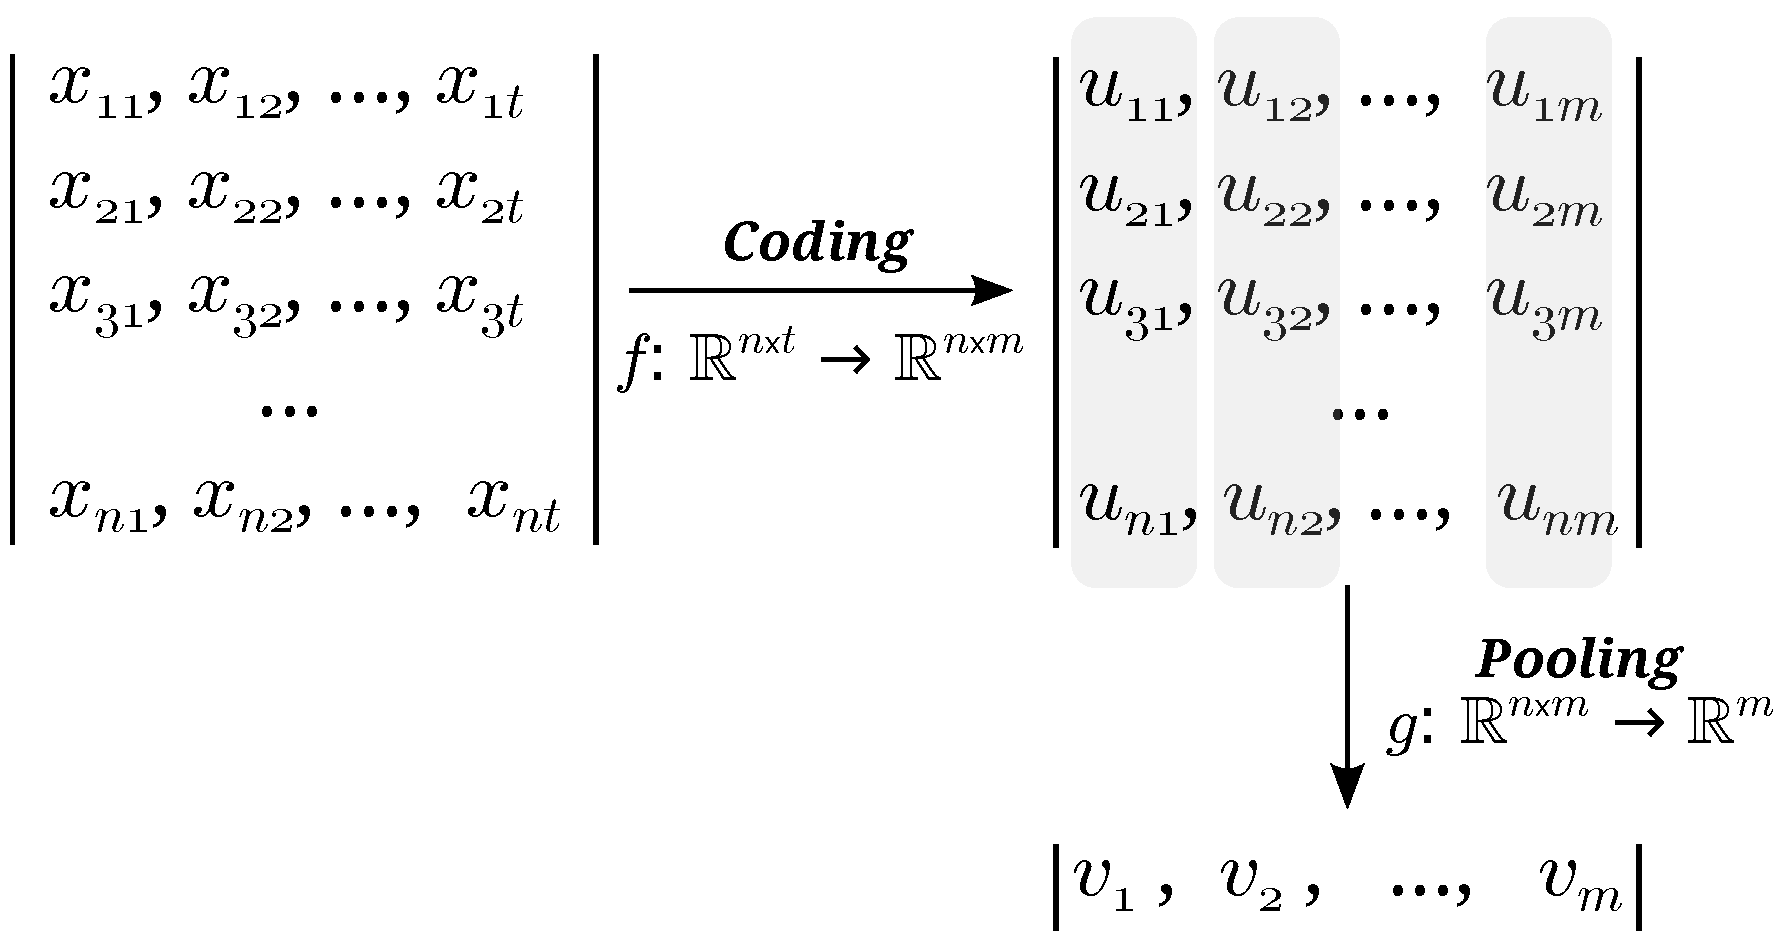
\includegraphics[width=0.48\textwidth]{coding_pooling_process.pdf}
%\caption{}
%\label{fig:coding_pooling_process}
%\end{figure}

\subsection{Classification}
After finding a new space representation for the videos in the database, we use machine learning algorithms \minor{to find} a classification model to decide whether a sample is an attempted attack or a valid access. In this paper, we evaluate the Partial Least Square (PLS)~\cite{Hoskuldsson:JC:1988} and Support Vector Machine (SVM)~\cite{Cortes:ML:1995} algorithms. 

%The PLS algorithm is a versatile data analysis tool applied in several research areas such as mathematics, economics, and computer science. PLS algorithm can be used in regression analysis, data visualization, dimensionality reduction, and data classification tasks. Similar to PCA~\cite{pearson1901lap}, the PLS is based on the linear transformation of the feature vectors to a new space formed by a small number orthogonal projection vectors. However, differently from PCA, the PLS projection vectors are chosen to maximize the covariance of the latent variables and the labels assigned to feature vectors~\cite{Schwartz:ICCV:2009}.
%
%SVM algorithm is a powerful state-of-the-art machine learning technique in many tasks of pattern recognition and computer vision. The SVM operation is based on the projection of the original space of the input feature vectors onto a higher dimensional feature space in order to find an optimal hyperplane that separates the input feature vectors into classes. SVM aims at finding the maximum margin hyperplane that separates two classes of interest. The found hyperplane can be represented as a linear combination of the input feature vectors, called support vectors, and the decision function to classify new feature vectors involves dot products between some input feature vectors. Therefore, SVM can find a separating hyperplane in the feature space and classify new feature vectors in that space without ever representing the space explicitly by means of a kernel function, which plays the role of the dot product in the feature space, avoiding explicit computations in the high dimensional feature space~\cite{James:STS:2013}.

\section{Experiments and Results}\label{sec:experimentalresults}
In this section, we present and discuss the experimental results and the validation of the proposed method. Section~\ref{subsec:Database} shows details of the datasets used in the experiments while Section~\ref{subsec:Protocol} describes the experimental protocols employed in this work. Section~\ref{sec:setup} shows the experimental setup of the proposed method regarding its parameters. The experiments in Section~\ref{subsec:analysis} aim at validating our method and choosing its best parameter setup. In addition, Section~\ref{subsec:analysis} addresses important questions regarding the low- and mid-level descriptor extraction procedures: {(1) the best characteristic extracted from Fourier spectrum (e.g., magnitude or phase spectrum); (2) the best measure for spectrum summarization (e.g., energy, entropy, correlation, mutual information, etc);} and (3) the visual codebook size most appropriate for the problem; among others. The remaining subsections compare the proposed method with the best methods reported in the literature including a challenging cross-dataset protocol, whereby we train our method using a dataset and test it with another dataset.

\subsection{Datasets}
\label{subsec:Database}
In this work, we consider four datasets:
%
\begin{itemize}
\item \textbf{Replay-Attack Dataset~\cite{Chingovska:BIOSEG:2012}}: This dataset comprises videos of valid accesses and attacks of $50$ identities. The videos were generated with a webcam with a resolution of $320 \times 240$ pixels and $25$ frames per second (fps). {This dataset contains $200$ valid access videos, $200$ print-based attacks, $400$ mobile-based attacks using an iPhone, and $400$ high-definition attacks using an iPad screen with $1,024 \times 768$ pixel resolution.}

\item \textbf{CASIA Face Anti-Spoofing Dataset~\cite{Zhang:ICB:2012}}: This dataset contains videos of valid accesses and attacks of $50$ identities and considers different types of attacks such as warped photo attacks and cut photo attacks, besides the photos and video attacks. It also considers attacks performed with different image/video quality: 
{(1)~low-quality videos captured by a long-time-used USB camera with $480 \times 640$ pixel resolution; (2) normal-quality videos captured with a new USB camera with $480 \times 640$ pixel resolution; and (3) high-quality videos captured with a Sony NEX-5 camera with $1,920 \times 1,080$ pixel resolution.} In total, it comprises $150$ valid access videos and $450$ video spoofing attacks.

\item \textbf{UVAD Dataset~\cite{Pinto:Unicamp:2013, Pinto:TIFS:2015}\footnote{This dataset is freely available through FigShare \allan{(http://figshare.com/articles/visualrhythm\_antispoofing/1295453)}.}}: This dataset contains valid access and attempted attack videos of {$404$ different people}, all created at Full HD quality, $30$ fps, and nine seconds long. It contains {$16,268$ attempted attack videos and $808$ valid access videos}. {Seven different display devices} were used to simulate the attempted attacks performed upon three acquisition sensors of different manufacturers: {a 9.1 megapixel (MP) Sony CyberShot DSC-HX1, a 10.0-MP Canon PowerShot SX1 IS, a 10.3-MP Nikon Coolpix P100, a 14.0-MP Kodak Z981, a 14.0-MP Olympus SP 800UZ, and a 12.1-MP Panasonic FZ35 digital camera. Figs.~\ref{fig:exemplosVideosValidos} and~\ref{fig:exemplosVideosAtaque} illustrate some examples of this dataset.}
%
\begin{figure*}[!htb]
\centering
\begin{tabular}{c}
	\includegraphics*[width=0.12\textwidth]{facesReais/MAH00938.PNG}
	\includegraphics*[width=0.12\textwidth]{facesReais/MAH01011.PNG}
	\includegraphics*[width=0.12\textwidth]{facesReais/MAH01205.PNG}
	\includegraphics*[width=0.12\textwidth]{facesReais/MAH01241.PNG}
	\includegraphics*[width=0.12\textwidth]{facesReais/MAH01502.PNG}
\end{tabular}
\caption{Examples of valid access video frames for outdoor (first and second images on the left) and indoor (three images on the right) scenes.}
\label{fig:exemplosVideosValidos}
\end{figure*}
%
\begin{figure*}[!htb]
\centering
\begin{tabular}{c}
	\includegraphics*[width=0.12\textwidth]{facesFakes/MAH00938.PNG}
	\includegraphics*[width=0.12\textwidth]{facesFakes/MAH01011.PNG}
	\includegraphics*[width=0.12\textwidth, height=0.082\textheight]{facesFakes/MAH01205.PNG}
	\includegraphics*[width=0.12\textwidth, height=0.082\textheight]{facesFakes/MAH01241.PNG}
	\includegraphics*[width=0.12\textwidth, height=0.082\textheight]{facesFakes/MAH01502.PNG}
\end{tabular}
\caption{Examples of attempted attack video frames for outdoor (first and second images on the left) and indoor (three images on the right) scenes using Sony (first and second columns), Canon (third and fourth columns) and Nikon (last column) cameras.}
\label{fig:exemplosVideosAtaque}
\end{figure*}

\item \textbf{3DMAD Dataset~\cite{Erdogmus:BTAS:2013}}: This dataset comprises valid access and mask attack videos of $17$ different subjects, whose faces were recorded by a Microsoft Kinect sensor. To build a synthetic biometric sample, the authors used frontal and profile face images to make the facial reconstruction. Afterwards, the authors used a 3D printer to build a mask containing facial information of the target person. Spoofing attack simulations were performed by presenting the 3D masks to the same Microsoft Kinect sensor. In total, the authors generated $85$ valid access videos and $85$ attempted attack videos.
\end{itemize}

\subsection{Experimental Protocol}
\label{subsec:Protocol}
We use \redmark{two measures for performance evaluation}: the area under the curve (AUC) and the half total error rate (HTER). \minor{While the former} quantifies the overall ability of a classifier to discriminate between attempted attacks and valid accesses, \minor{the latter} combines the false acceptance rate (FAR) and false rejection rate (FRR) in a specific operating point of the ROC curve into a single measure. HTER is commonly calculated in the operating point in which the FAR is equal to the FRR, known as the Equal Error Rate (EER). \redmark{We use the freely available toolbox Bob~\cite{Anjos:ACMMM:2012} to calculate the AUC and HTER values. Finally,} the employed evaluation protocols follow the ones proposed by the authors of the Replay-Attack, \allan{CASIA,} UVAD and 3DMAD datasets. The source code of all proposed methods are freely available.\footnote{{The source code is freely available for scientific purposes on GitHub \allan{(https://github.com/allansp84/spectralcubes)}, along with this article.}}

\subsubsection{Protocol I} In this experimental protocol, we use the Replay-Attack dataset, which is divided into three subsets: a training set with $300$ attack videos and $60$ valid videos; a development set with $300$ attack videos and $60$ valid access videos; and a test set with $400$ attempted attack videos and $80$ valid access videos. \minor{The training set is used to fit a classification model, the development set to find the EER, whereas the test set is used to report the final error rates.}

\subsubsection{Protocol II} \minor{In this protocol, we use CASIA dataset, divided into two disjoint subsets: training and test sets. \allan{Due to the absence of a development set to estimate a threshold to be applied in the test set and afterwards to calculate the HTER, the official protocol of this dataset recommends to use the training set to build a classifier and then use the test set to report the EER value. To report the results in terms of HTER, the original training set was divided into two subsets, named as training and development sets, in the proportion of $80\%$ and $20\%$, respectively. We use the new training set to find the classification model and the development set to estimate the threshold that gives us the EER, whereas the official test set is used to report the final results in terms of HTER.}
}


%\subsubsection{Protocol II} This is a protocol similar to Protocol I except that we use CASIA dataset instead of Replay-Attack. This dataset is already divided into training and test sets. We split the training into 80\% for actual training and 20\% for development (parameter {optimization}). Finally, the {official} test set was used as the test set.

%\subsubsection{Protocol III} In this protocol, we use the UVAD dataset, which contains one subset with $304$ valid access videos and three subsets, each one with $2,343$ attempted attack videos. Each subset contains attempted attack videos that were generated through spoofing attacks performed in a face biometric system equipped with one of three sensors: Sony, Canon, or Nikon. We use a cross-dataset evaluation protocol here in which we train the classification model with the Replay-Attack dataset and we use UVAD valid access and attempted attack videos to perform the test.

\subsubsection{Protocol III} \minor{In this protocol, we use the UVAD dataset, which contains six subsets comprising valid access and attempted attack videos. Each subset considers attacks against one acquisition sensor: Sony, Kodak, Olympus, Nikon, Canon and Panasonic. Here, we train a classifier using the sensors Sony, Kodak and Olympus, and we test it with videos (valid access and attempted attacks) from three other different manufacturers: Nikon, Canon and Panasonic.}

\subsubsection{Protocol IV} \minor{Here, we use the 3DMAD dataset to evaluate spoofing detection of attacks using 3D masks. The dataset contains $85$ RGB videos that represent valid access and $85$ RGB videos that represent attempted spoofing attacks. As this dataset does not contain explicit subsets, we randomly partitioned the data into three subsets: training, development and testing, and we use Protocol I for testing.}

\subsection{Method Parameterization}\label{subsec:setup}
\label{sec:setup}
For reproducibility purposes, \minor{this section discuss} the parameters whose values are constant in the setup of our method. 

We extract the \redmark{noise signature} from RGB videos using a Gaussian filter with~$\mu = 0$,~$\sigma = 0.5$, and kernel size~$ 3 \times 3$ (Eq.~\ref{eq:ruido}). These values were obtained empirically in~\cite{Pinto:SIBGRAPI:2012}. Next, we extract cuboids of size $32 \times 32 \times 8$ from the Fourier spectrum videos (Eqs.~\ref{eq:mag_spectrum} and~\ref{eq:phase_spectrum}), whose spatio-temporal location is \redmark{chosen randomly based on} a uniform distribution. 

The use of spatial measures produces {low-level $8$-dimensional descriptors} per channel, whereas the use of spatio-temporal measures produces low-level $7$-dimensional descriptors per channel, which gives us a final low-level descriptor of $24$-dimensional and $21$-dimensional, respectively. Finally, the number of cubes extracted from videos is determined by dividing the volume of the video with respect to the cube.

\redmark{Regarding the mid-level descriptors}, the only parameters with constant values are the ones that define the Gaussian kernel used in the soft-assignment coding technique, whose values are~$\mu = 0$ and~$\sigma = 0.04$. Finally, the SVM parameters are found through grid search in  the training data.

\subsection{Experimental Design and Analysis}\label{subsec:analysis}

\begin{table*}
\begin{center}
\begin{footnotesize}
\footnotesize
\caption{{After the statistical analysis, we have found that the factors highlighted with $\dagger$ are the ones that did not present statistical significance when configuring our method, whereas the levels highlighted in bold are the chosen levels.}}
\label{table:DOE}
\begin{tabular}{lp{3.0cm}p{0.70\textwidth}}
\topline
\headcol \textbf{Factor} & \textbf{Levels} & \textbf{Description} \\
\midline
\multirow{1}{*}{LGF} & C, and \textbf{W} & Strategies for extracting the low-level features from video of phase spectrum or video of magnitude spectrum: extraction considering a central region (crop) in each frame (C) and the entire/whole frames (W).\\
\hline
\rowcol \multirow{1}{*}{M} & PE, PH, ME, MH, PMI, MMI, PC, and \textbf{MC} & Characteristics of the frequency spectrum evaluated that can be the phase (P) or magnitude (M) and the measures used for summarizing the spectral information that can be {energy (E), entropy (H), mutual information (MI), or correlation (C)}.\\
\hline
\multirow{1}{*}{CS} & R, and \textbf{K} & Mode of selection of the visual words that compose the visual codebooks: Random (R) or using $k$-means clustering algorithm (K). \\
\hline
\rowcol \multirow{1}{*}{SDD$^{\dagger}$} & S and D & Strategies for generating the visual codebooks: a single visual codebook (S) and class-based visual codebooks (D), one for each data class (spoofing vs non-spoofing). \\
\hline
\multirow{1}{*}{DS$^{\dagger}$} & $80$, $120$, $160$, $200$, $240$, $280$, $320$, and $360$ & Visual codebook sizes. This is an important parameter because the visual codebook size gives us visual codebooks with different degrees of specificities because large visual codebooks can incorporate small clusters of data that appear sometimes in specific cases. \\
\hline
\rowcol \multirow{1}{*}{CP} & hardsum, hardmax and \textbf{softmax} & We evaluate the combination of two strategies in the coding process (hard-assignment and soft-assignment) and two strategies in the pooling process (max-pooling and sum-pooling). \\
\hline
\multirow{1}{*}{C} & \textbf{SVM} and PLS & Classification algorithms. \\
\bottomline
\end{tabular}
\end{footnotesize}
\end{center}
\end{table*}

\redmark{To find the \minor{best method configuration}, we performed} a factorial experiment with replication ($N=3$) followed by an analysis of variance (ANOVA)~\cite{Walpole:PE:2007}. Each experimental unit is represented as a tuple of $n$ objects, each one with a level of a factor. Considering the replications, we have a total of {$9,216$ tuples}, which are used to instantiate the proposed method. The instances of the proposed method are evaluated through the measurement of the value of the system response variable, the AUC value, after running such instances using the Replay-Attack dataset and Protocol~I, using the development set. Next, we collect \redmark{obtained AUC values and then} we performed an ANOVA test to analyze the significance of the effects of the parameters on the \redmark{classification results}. 

With this approach, we can discover which parameters significantly affect the system response variable and also the best configuration of the method~\cite{Hayter:CL:2012}. Henceforth, the \minor{method parameters} are referred to as \emph{factors} and their values as \emph{levels}. Table~\ref{table:DOE} shows a brief description of the factors and their respective levels we consider herein. 

\subsubsection{Low-Level Descriptor Extraction Parameter Analysis (LGF and M)}\label{sec:main_effect_1}

\minor{The low-level feature extraction has two important parameters: the frequency characteristics of the signal (phase or magnitude), and the function used to summarize the information of the temporal cubes extracted from a video. In this work, we evaluate measures that describe spatial information of the temporal cubes (energy an entropy), and measures that describe the temporal behavior of the cubes (mutual information and correlation across time).}

\minor{To find which levels are statistically different for each factor, we perform the Tukey's HSD test (see Fig.~\ref{fig:llf_pvalues}). \redmark{In Figs.~\ref{fig:llf_pvalues}(a)-(b)}, the pairs in comparison whose confidence intervals do not intercept the zero value are statistically different. \allan{Considering the top-5 method configuration obtained in this experiment, we conclude that} the whole frame for extracting features is more interesting than any cropped region in the center of the frame. In addition, the characteristic extracted of the Fourier spectrum and the summarization measure used to generate the low-level feature descriptors \allan{have a great impact} in the method discriminability (Fig.~\ref{fig:llf_pvalues}(b)), \allan{as several comparisons in pairs of features are statistically significant.}}
%
\begin{figure*}[!ht]
\centering
\subfloat[LGF denotes the region of the frame for extracting the low-level features.]{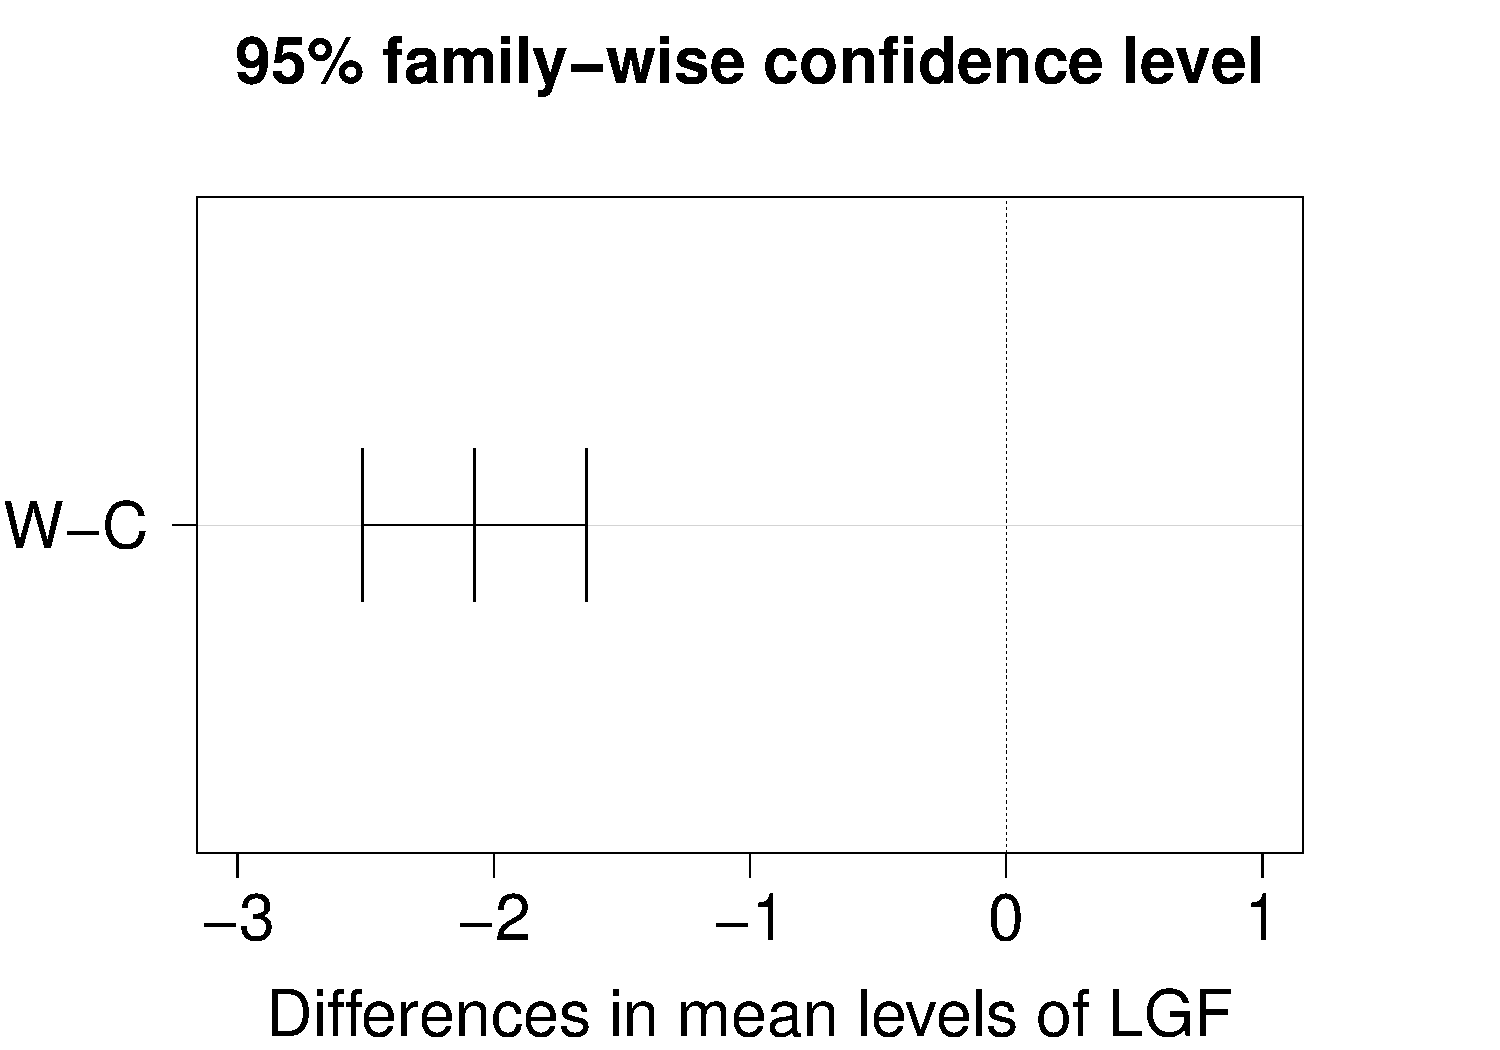
\includegraphics[width=0.21\textwidth]{test_0_auc/LGF}}\hspace{1cm}
\subfloat[M refers to summarization measure and the video of spectra used to generated the low-level descriptors.]{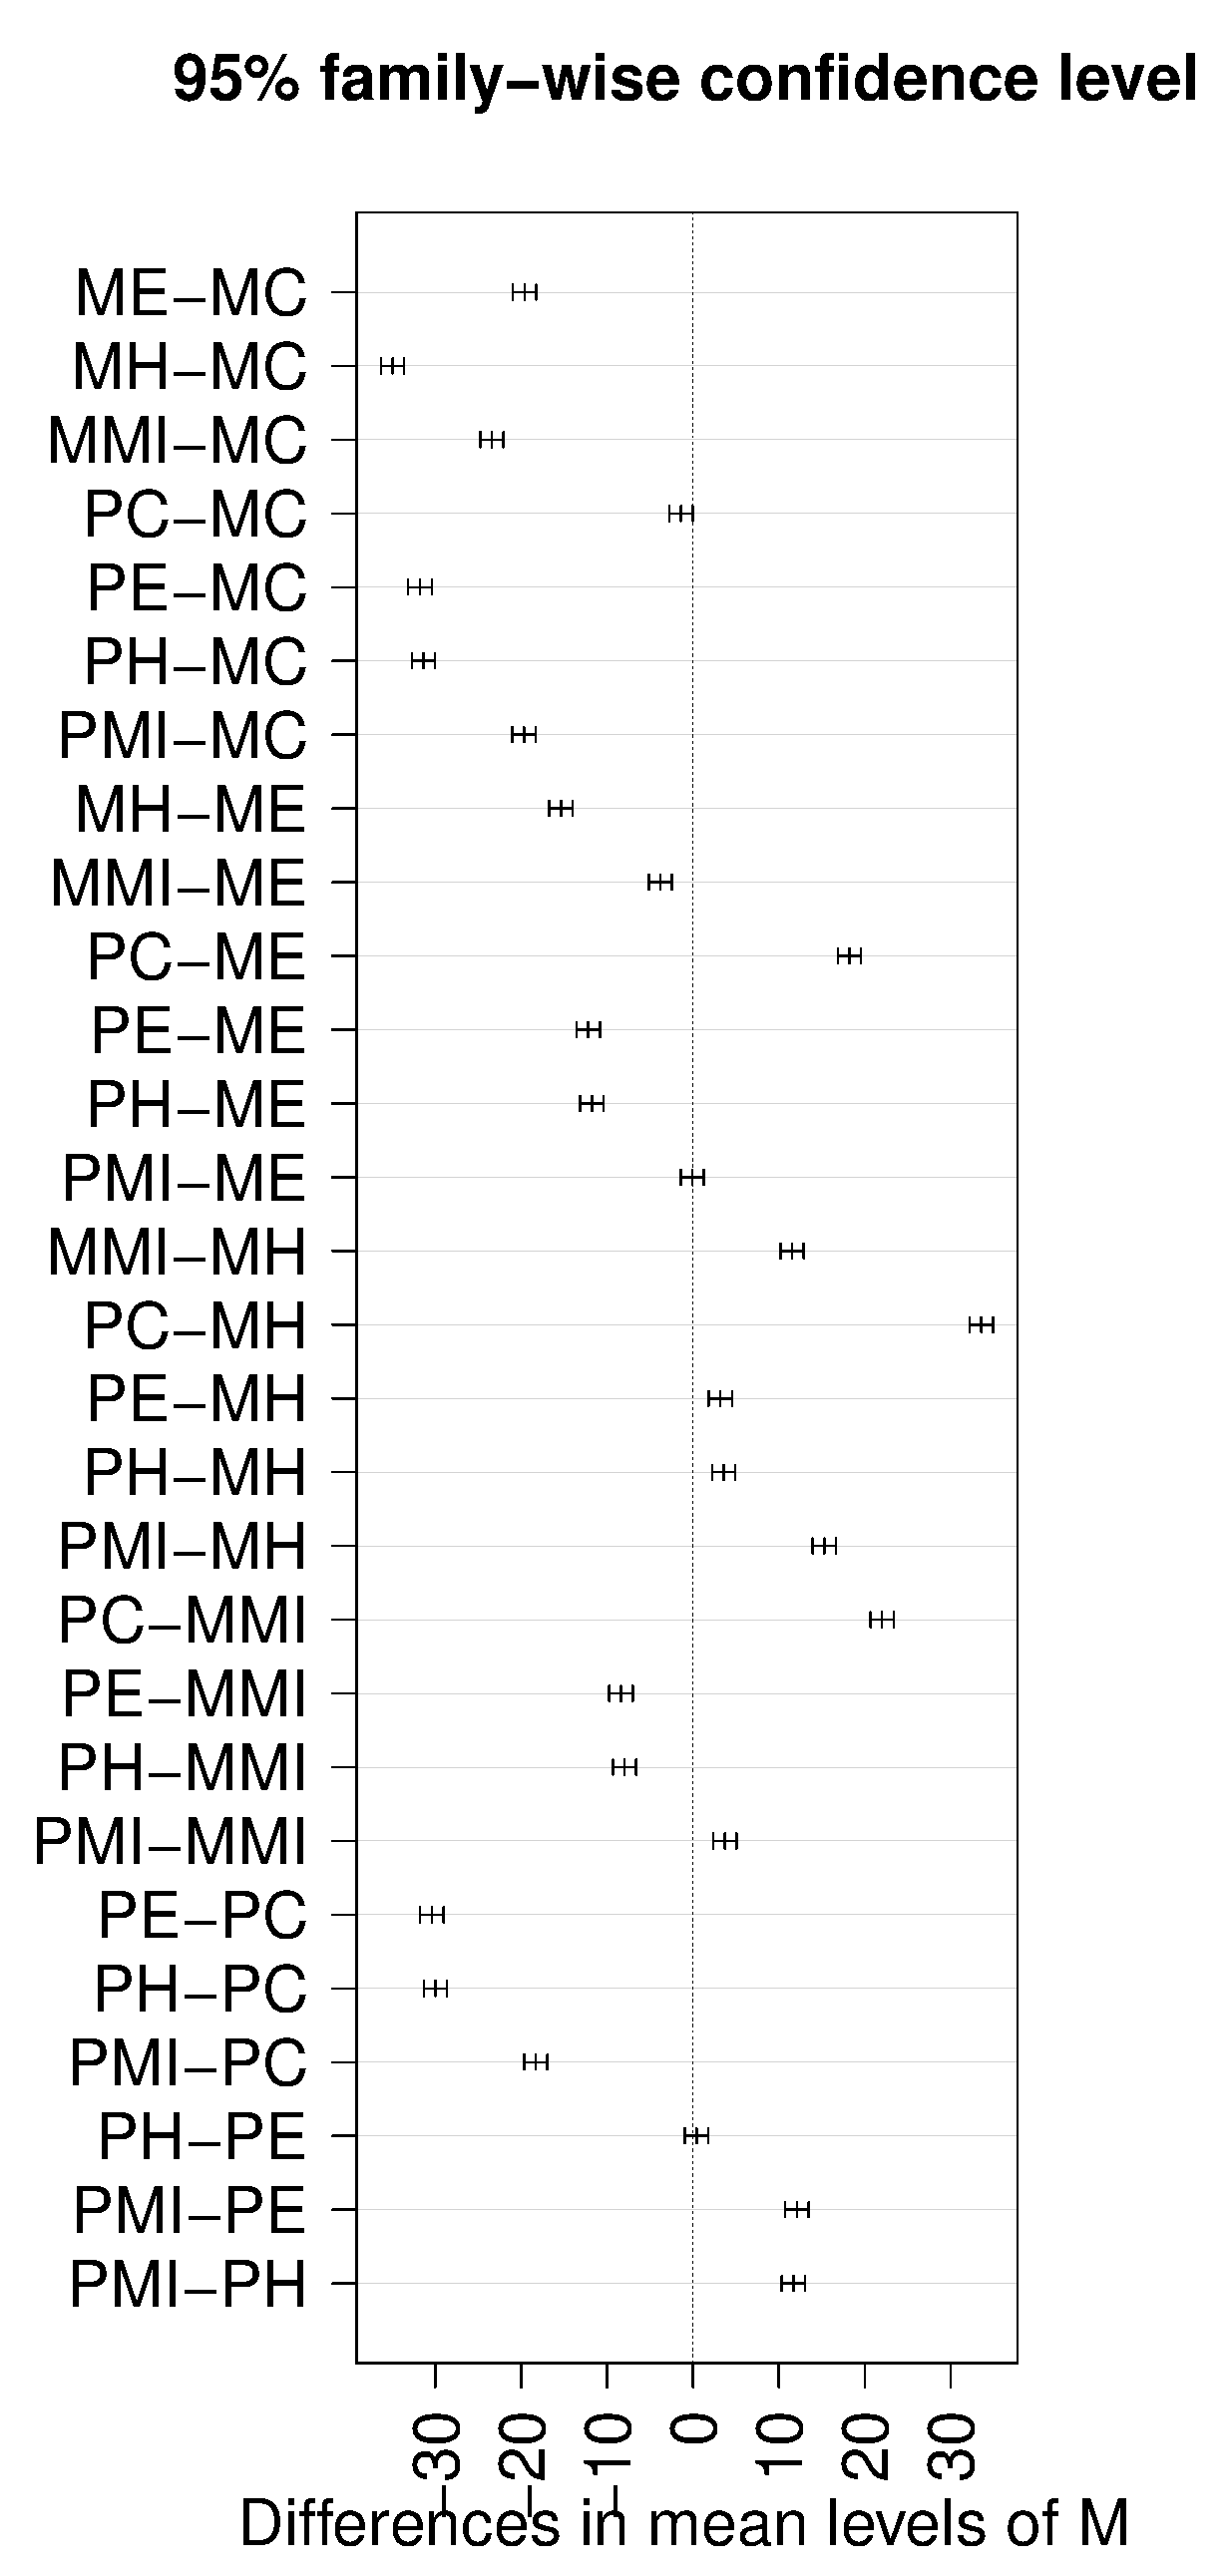
\includegraphics[width=0.35\textwidth]{test_0_auc/M}}\\
\caption{{Confidence interval on the differences between the means of the levels of the factors (a) LGF, and (b) M. For each comparison, the Tukey's HSD test provides an estimation of the differences between mean pairs and their respective confidence intervals, as well the $p$-value for each comparison. All comparisons whose confidence intervals do not contain zero value have a $p$-value lower than $0.05$ and, therefore, are statistically different with a $95\%$ confidence level. (See Table~\ref{table:DOE} to see the description of levels.)\label{fig:llf_pvalues}}}
\end{figure*}

\subsubsection{Mid-Level Descriptor Extraction Parameter Analysis (CS, SDD, DS, and CP)}\label{sec:main_effect_2}
\minor{To construct a discriminative visual codebook, we need to choose the best strategy for selecting the words that compose the visual codebooks (CS) as random or clustering-based,  the visual codebook size (DS), the policy to create the visual codebooks (SDD) as single or class-based, and the pooling and coding strategies (CP).}
%
\begin{figure*}[!ht]
\centering
\subfloat[DS refers to the number of time-spectral visual words present in the visual codebook.]{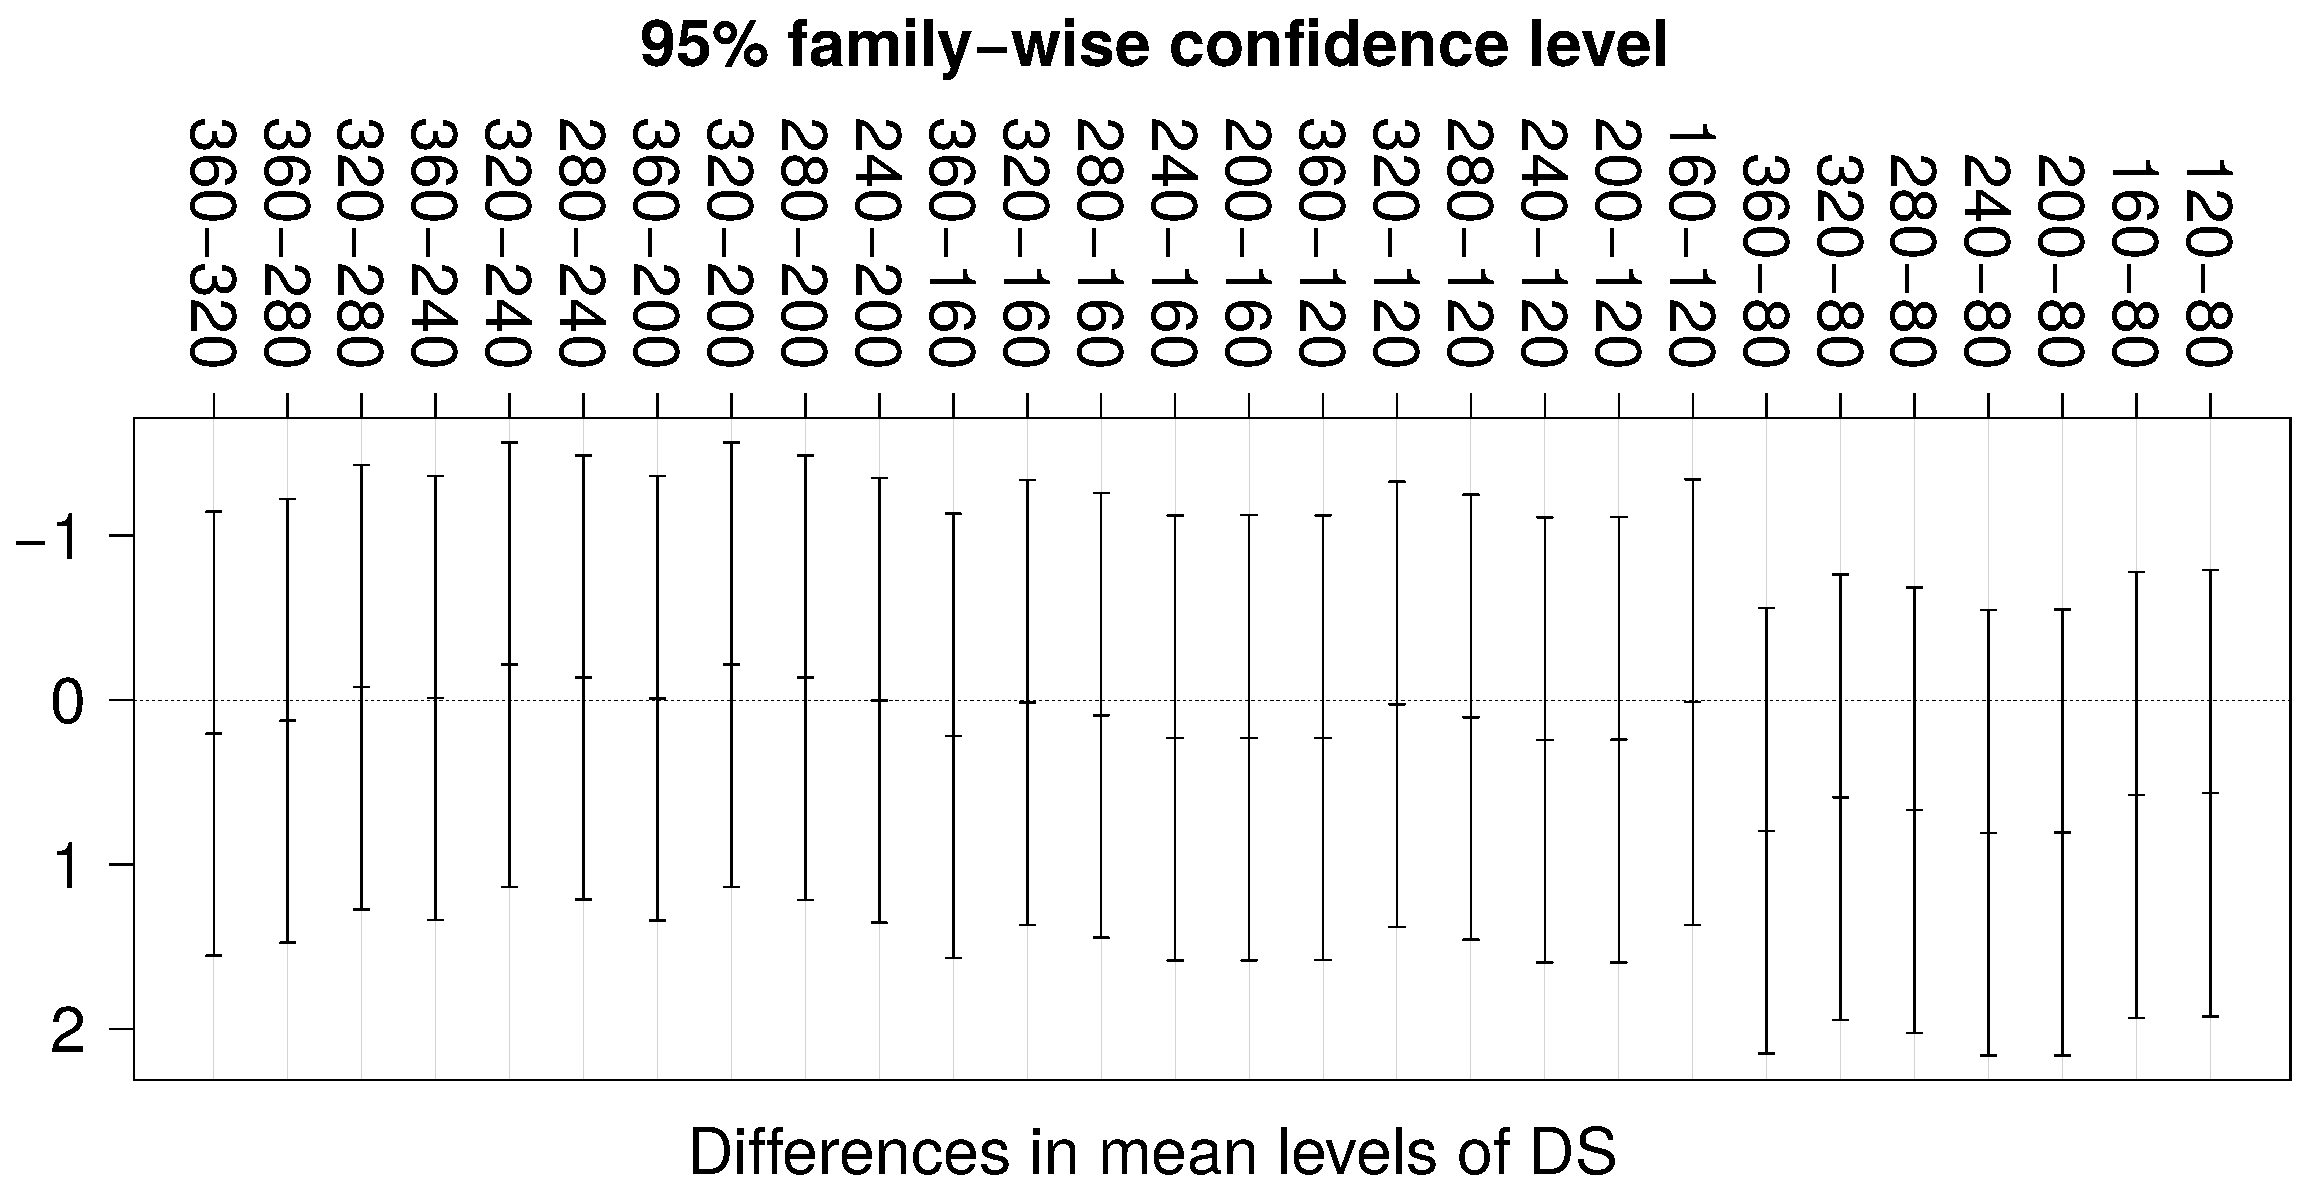
\includegraphics[width=0.3\textwidth]{test_0_auc/DS}} \\
\subfloat[CP denotes the coding and pooling strategies used to build the mid-level descriptors.]{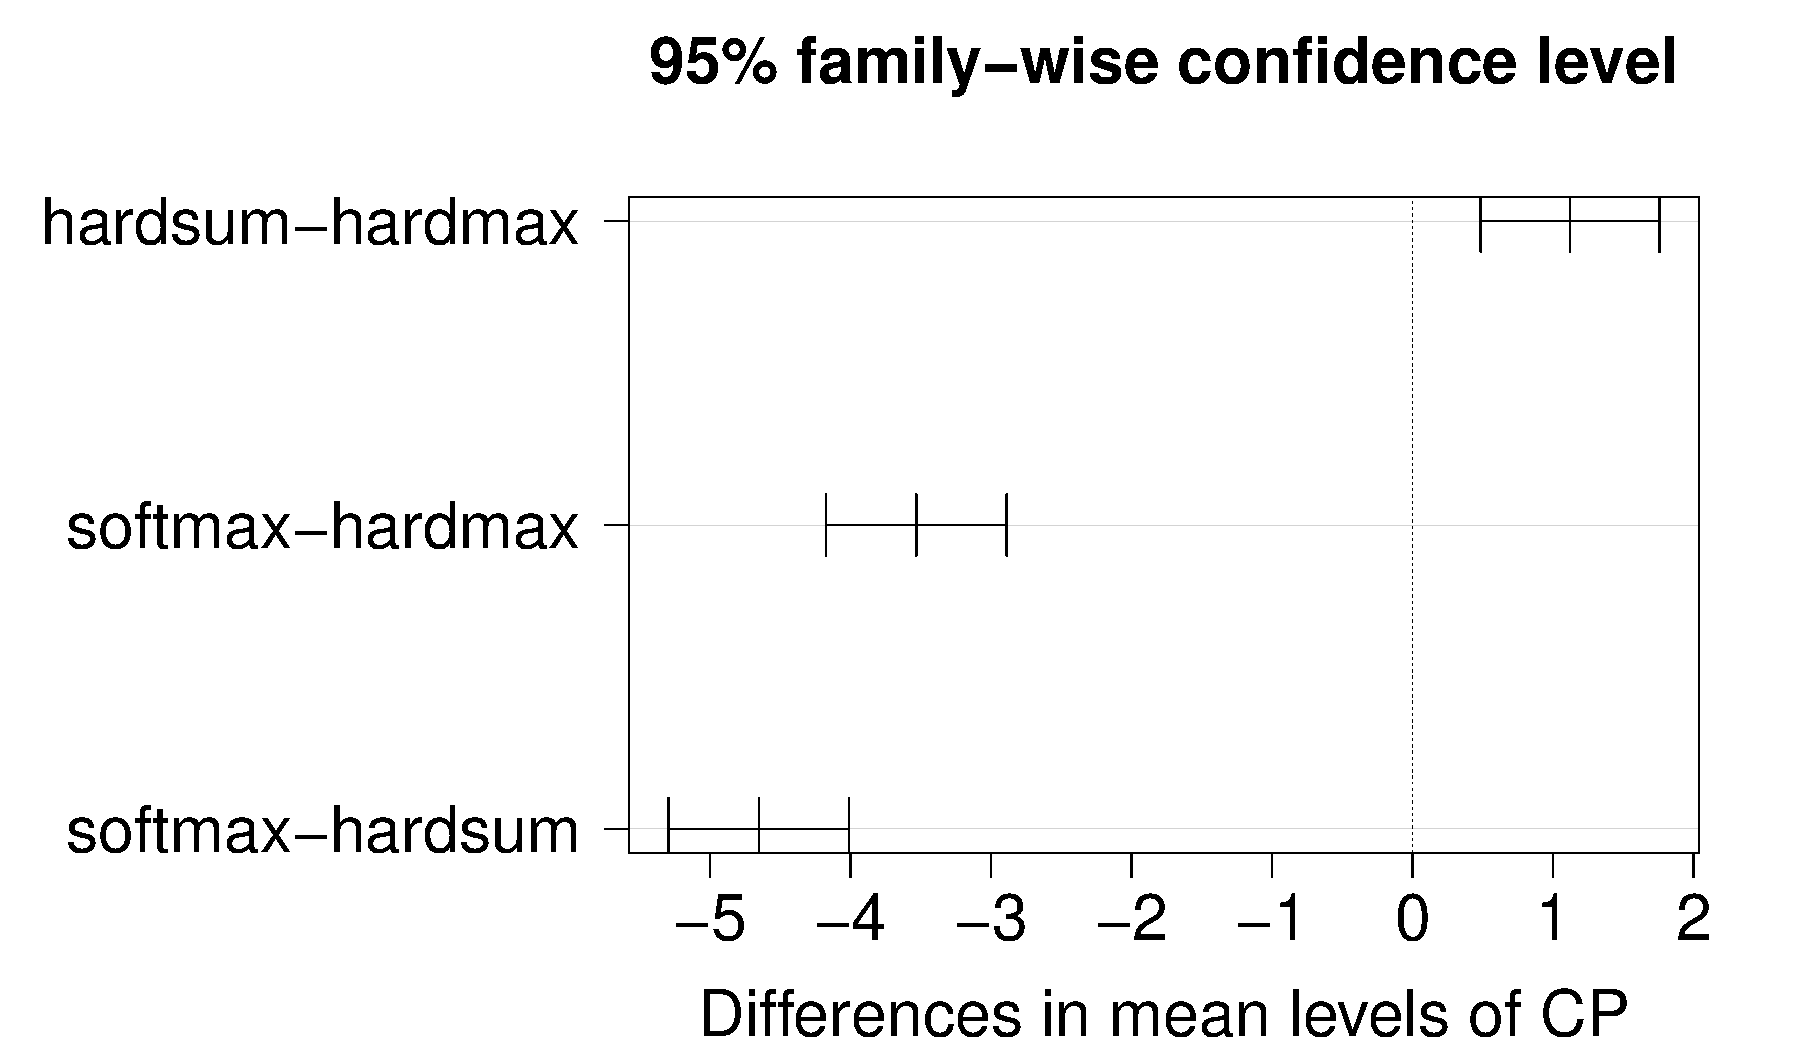
\includegraphics[width=0.25\textwidth]{test_0_auc/CP}}\hspace{5mm}
\subfloat[CS denotes the selection mode of the time-spectral visual words for composing the visual codebook.]{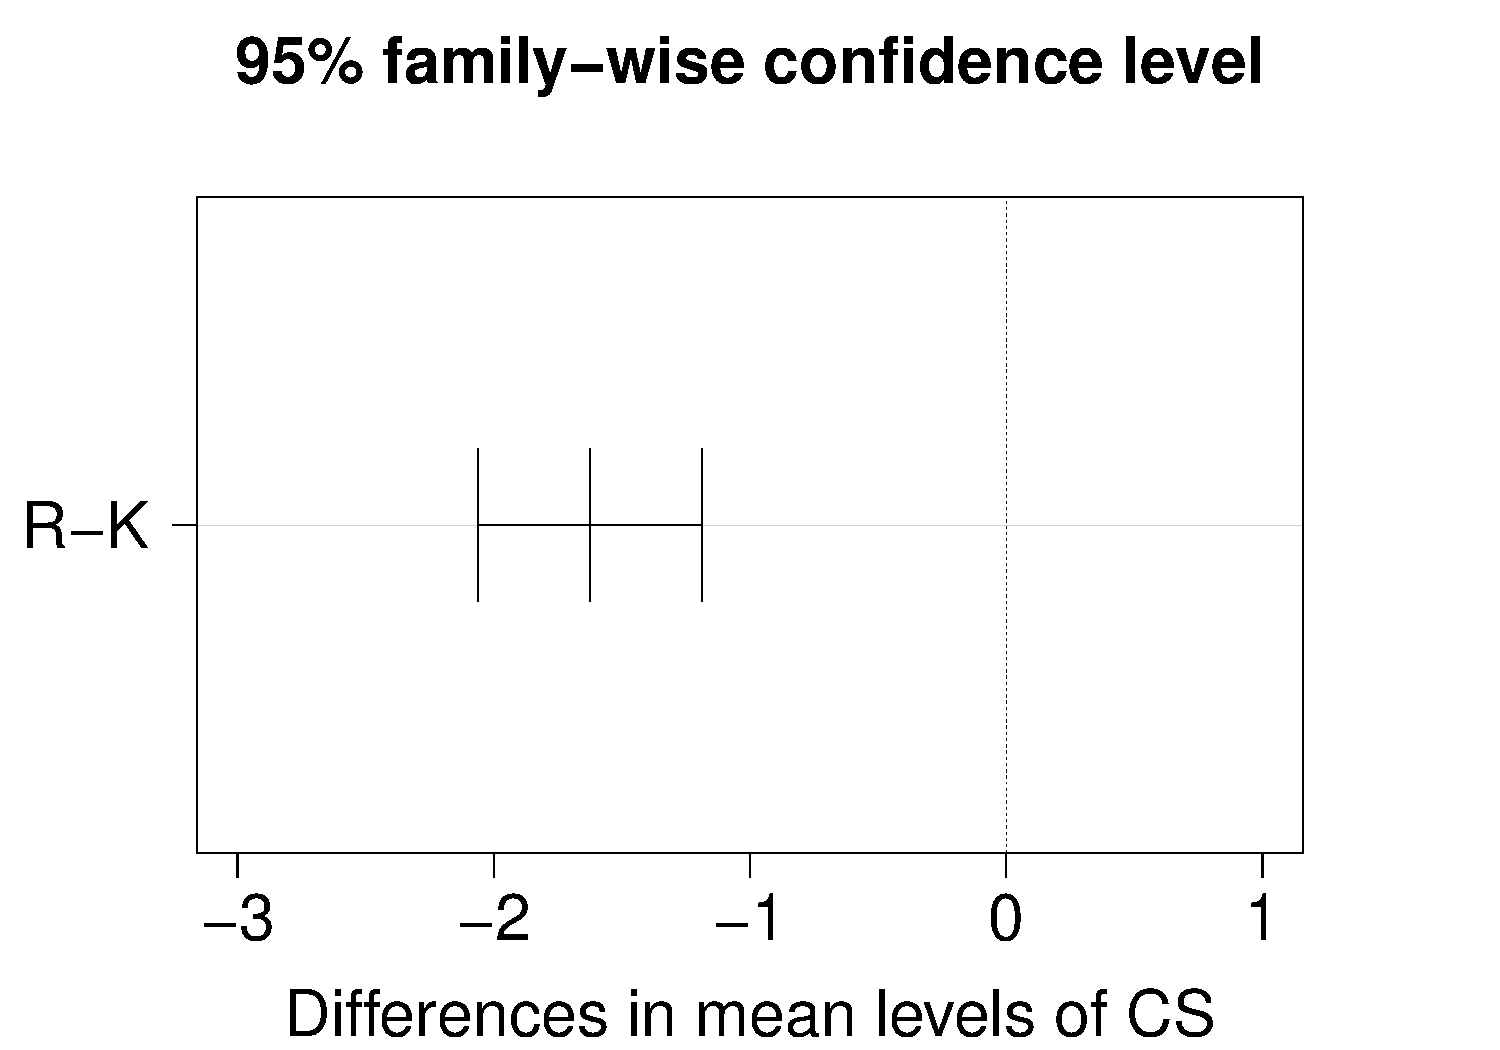
\includegraphics[width=0.22\textwidth]{test_0_auc/CS}}\hspace{2.5mm}
\subfloat[SDD denotes the strategies for generating the visual codebooks, single or class-based visual codebooks.]{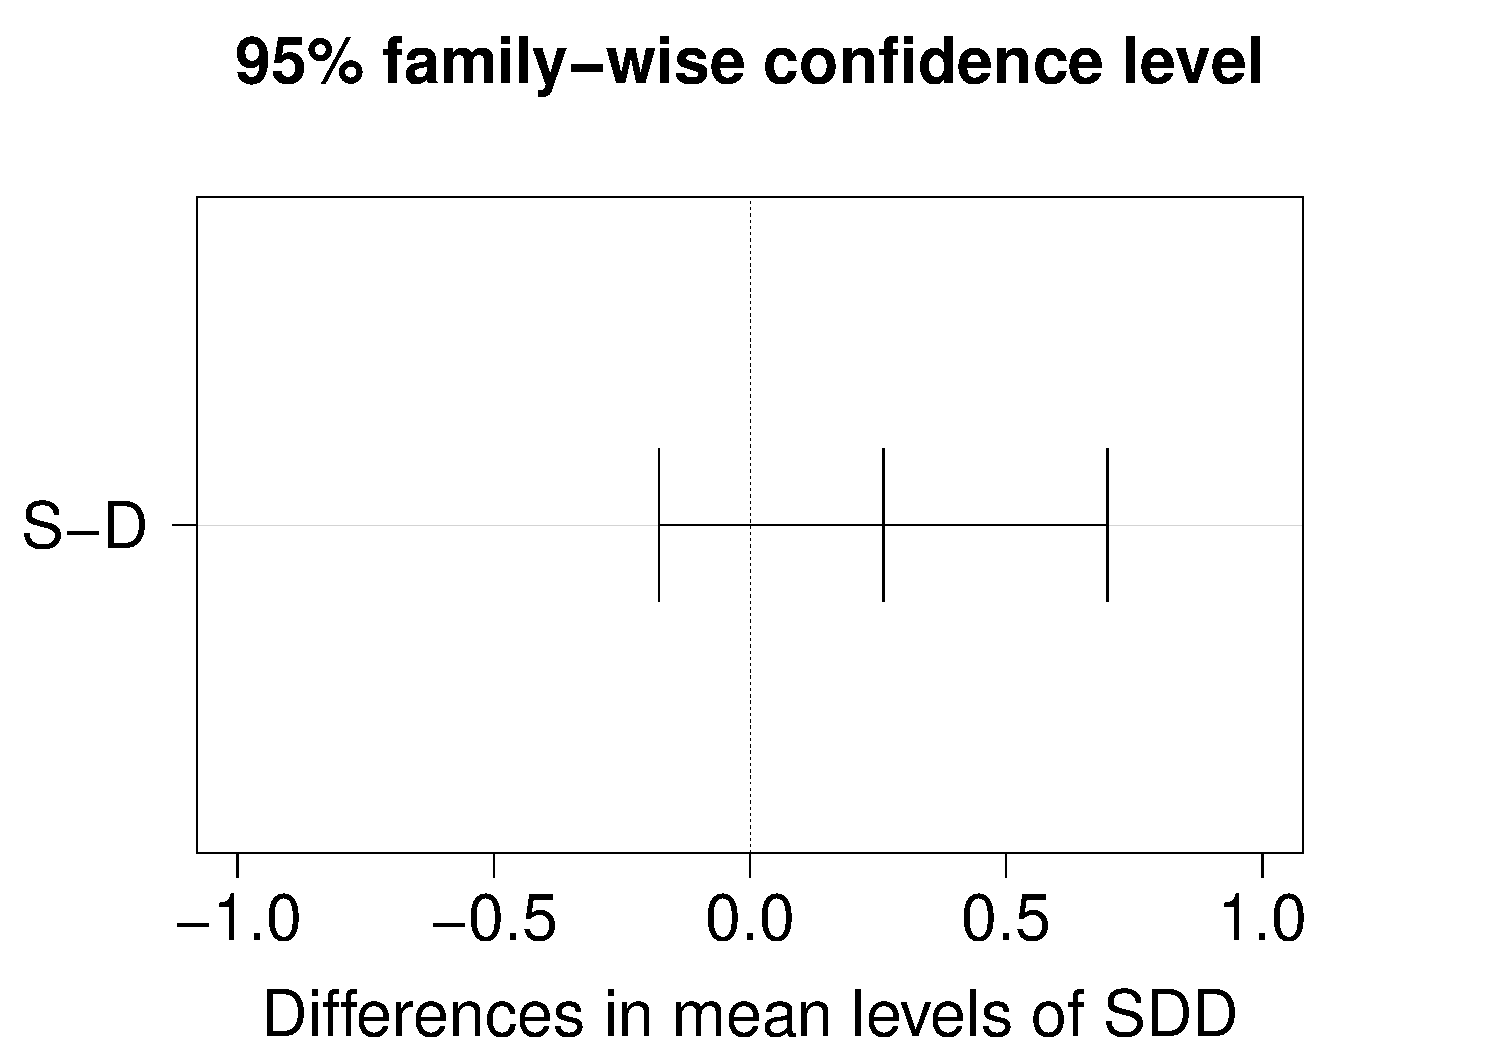
\includegraphics[width=0.2\textwidth]{test_0_auc/SDD}} \\
\caption{Confidence interval of the differences between the means of the levels of the factors (a) DS, (b) CP, (c) CS and (d) SDD. 
All comparisons whose confidence intervals do not contain zero value have a $p$-value lower than $0.05$ and, therefore, are statistically different with a $95\%$ confidence level as it is the case for the comparisons indicated on the (a) $x$ axis and (b-d) $y$ axis. (See Table~\ref{table:DOE} for the description of levels.)}
\label{fig:flf_pvalues}
\end{figure*}

\minor{Fig.~\ref{fig:flf_pvalues} shows the results of the post-hoc test with Tukey's HSD. {In Fig.~\ref{fig:flf_pvalues}(a), we have the results of the statistical analysis for DS parameter (dictionary size), to which was not found statistical significance}. Therefore, we recommend that dictionary size parameter to be optimized according to the application of interest. In turn, Fig.~\ref{fig:flf_pvalues}(b) shows that different pooling and coding processes causes statistically significant impacts on the response variable, and softmax is the recommended choice.}

\minor{In addition, Fig.~\ref{fig:flf_pvalues}(c) shows that the method used to select the words that compose the visual codebook (random vs. clustering-based selection) also presents results that are statistically {significant} with $k$-means being the recommend choice \allan{due to the high performance achieved by models built with visual codebooks generated using $k$-means, during this experiment}. Finally, Fig.~\ref{fig:flf_pvalues}(d) shows that the visual codebook creation strategy (single visual codebook vs. class-based codebooks) does not present statistical difference and, therefore, should also be considered in a future optimization process during the implementation of the method in a real application.}

\subsubsection{Classification Step Parameter Analysis (C)}\label{sec:main_effect_3}
The SVM classifier outperformed PLS classifier with a statistically significant difference  (\textit{$\textit{p}$-value} = $0.00$). We believe that this happened because of the non-linearity of the data as we use a non-linear version of SVM the a linear version of PLS.

\subsubsection{Analysis of Interaction Effects and Choice of the Best Configuration}
\label{sec:best:config}
\minor{After analyzing each factor in isolation, we examine whether there is significant interaction between factors}. In this case, if a small $p$-value is obtained in the interaction effect analysis between two factors, then we can conclude that these factors do not operate independently of each other~\cite{Hayter:CL:2012}. \redmark{Otherwise, there is no evidence of an interaction effect.} 

\minor{First of all, we can see that there is a relationship between the region from which the low-level time-spectral features are extracted (factor LGF) and the spectral information used in the generation of time-spectral descriptors (factor M). When analyzing the magnitude spectrum of the Fourier transform, we see that there is a concentration of low frequency components in the abscissa and ordinate axes. Fig.~\ref{fig:interactions} shows that this interaction between factors LGF and M exists. In addition: (i) we have an increase in the mean of AUC values for measures $MH$, $PH$, $PE$ and $PMI$, when these measures are calculated in the center region of the frames; (ii) we have a decrease in the mean of AUC for measure $PC$; and (iii) we have very small changes in mean values of AUC for $MC$ and $MMI$ when we compare the two strategies for feature extraction.}
%
\begin{figure}[!htb]
\centering
\subfloat[LGF and M interaction. Note that we have a slump in the mean of AUC when setting LGF to W and decrease the number of low-level features.]{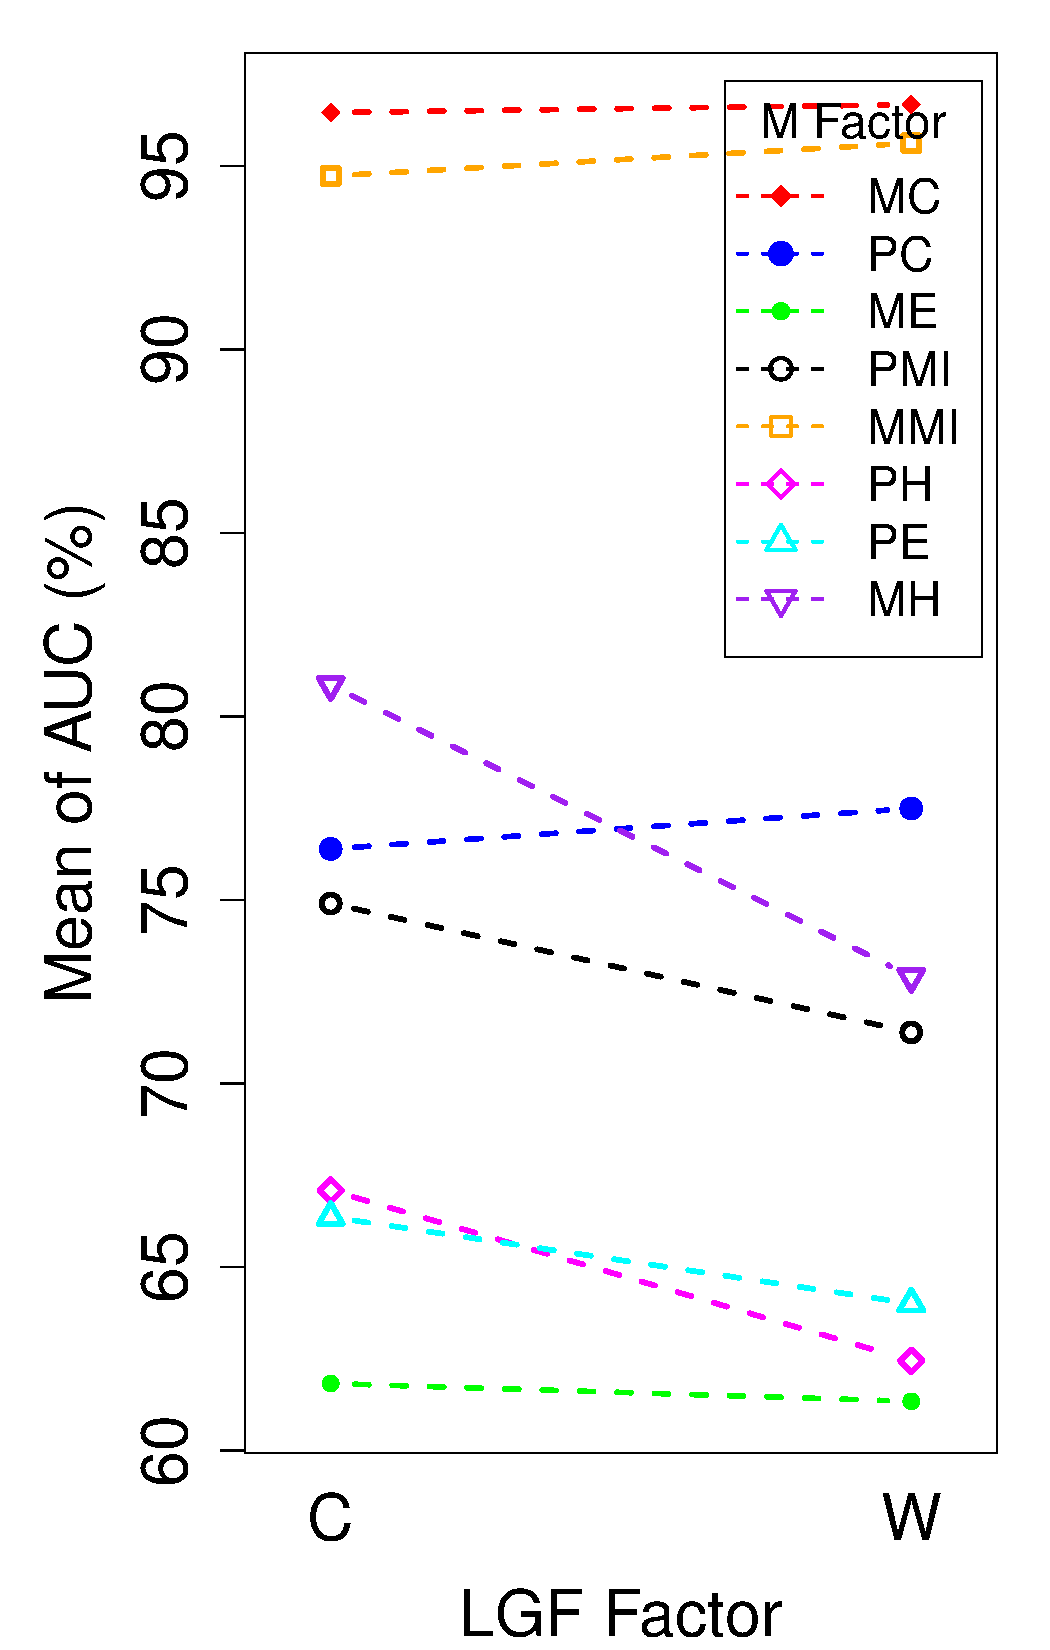
\includegraphics[height=4cm,width=3.5cm]{test_0_auc/LGF_M}}\hspace{0.5mm}
\subfloat[CS and CP interaction. We have a significant increase in the mean of AUC with the hard-assignment when we use $k$-means to select the visual words of the codebooks.]{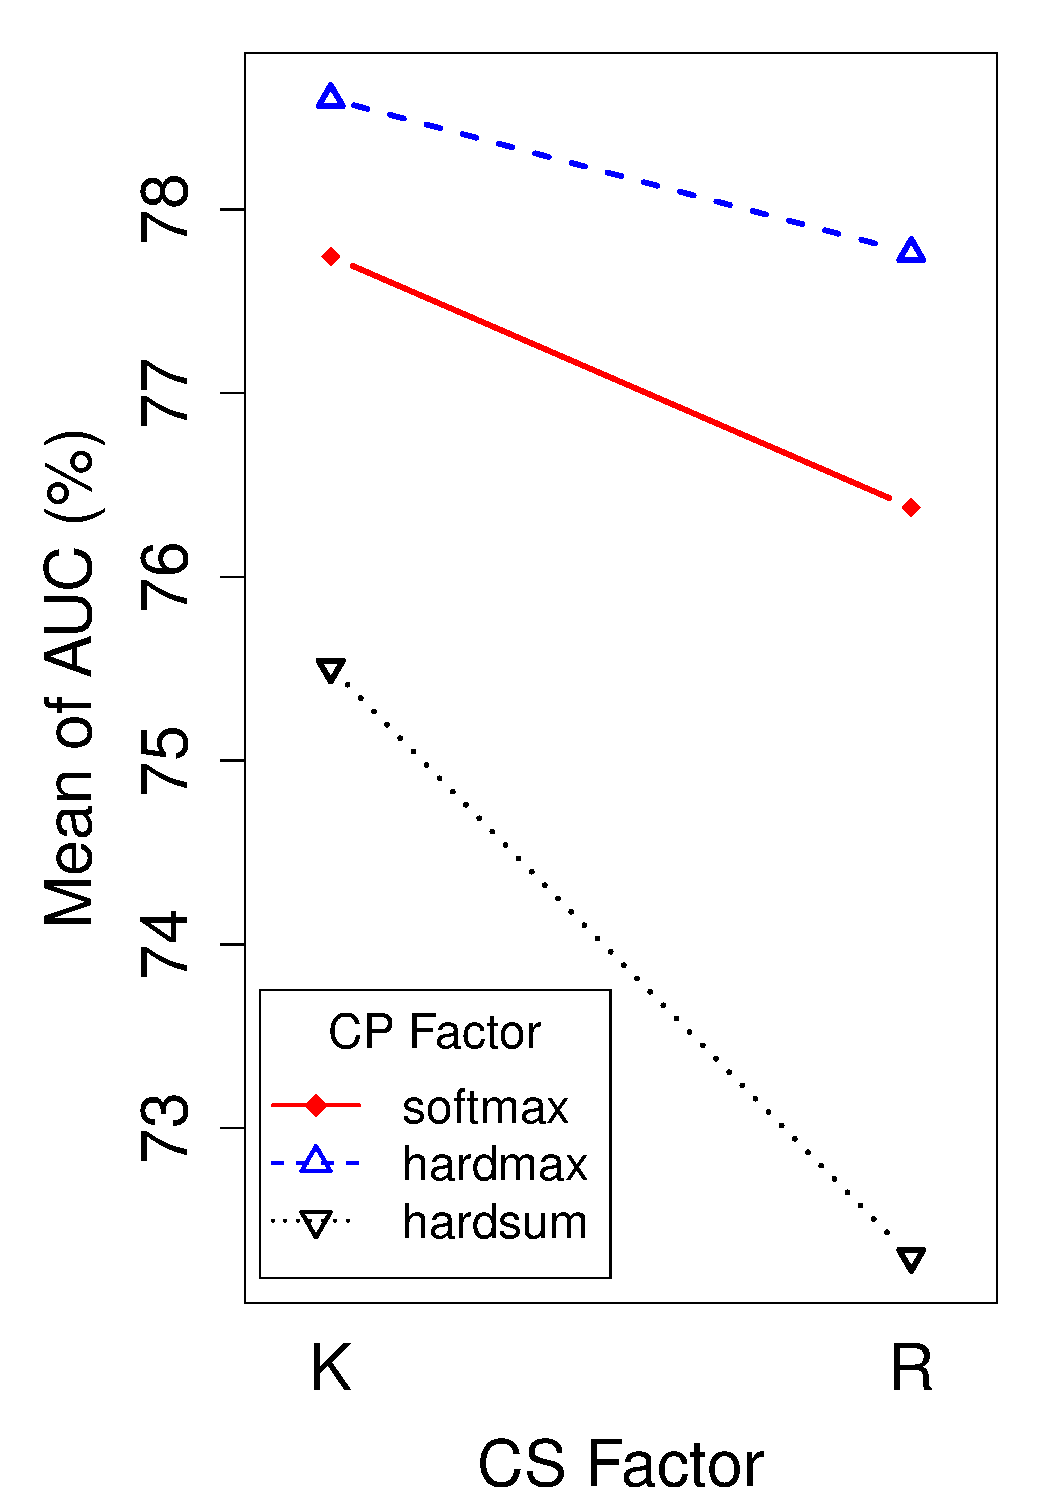
\includegraphics[height=4cm,width=3.5cm]{test_0_auc/CS_CP}}\hspace{0.05mm}
\caption{{Interaction plots between pairs of factors (a) LGF$\times$M and (b) CS$\times$CP. The factor LGF denotes the region in the frame considered for extracting the low-level features, while factor M denotes the statistical measures considered for describing the information of the temporal cubes. Finally, the factor CS denotes the mode of selection of the visual words {from visual codebooks} and the factor CP refers to the strategies used in the coding and pooling process. (See Table~\ref{table:DOE} to see the description of levels.)}}
\label{fig:interactions}
\end{figure}

Finally, the form of selecting the visual words (factor CS) and the method of coding and pooling used in the construction of the dictionaries (factor CP) also presents an interesting interaction. Both factors significantly influence the results, but not in isolation. Fig.~\ref{fig:interactions}(b) shows that the results obtained with hardmax, hardsum and softmax are worse when the visual words are chosen randomly instead of through clustering. 

\subsection{Summary After Analyzing Different Factors and Levels}
{The proposed method presents better results using time-spectral features extracted from magnitude spectrum videos considering the whole frames of a video and using the correlation measure from time-spectral features for generating the time-spectral descriptors.}

{The class-based codebooks \minor{outperform} the single codebook and the selection strategy of the visual words that best fits to the spoofing detection problem is the $k$-means clustering. The most appropriate size for codebooks is $320$ visual words and the softmax outperformed the other coding and pooling strategies. With this configuration, we obtained an AUC of $99.46\%$ and an HTER of $2.75\%$, considering the \allan{test set} of the Replay-Attack dataset~\cite{Chingovska:BIOSEG:2012}. Next, we show experiments and results for this method using this final configuration.}

\subsection{Results}\label{subsec:soa_comparison}
\minor{This section compares the proposed method with others in the literature for the {Replay-Attack~\cite{Chingovska:BIOSEG:2012}, CASIA~\cite{Zhang:ICB:2012} and 3DMAD~\cite{Erdogmus:BIOSIG:2013} datasets. In all experiments, we used the best configuration of the proposed method as discussed in the last section. The parameters that did not present statistical significance (DS and SDD), were fine-tuned for each dataset.}}

\subsubsection{Replay-Attack Dataset}\label{subsec:ra_results}

\minor{We first consider the validation Protocol I~(c.f., Sec.~\ref{subsec:Protocol}) and the Replay-Attack dataset. Table~\ref{table:our_reults} shows the results for the three types of attacks available in this set. Fig.~\ref{fig:det_plot_replay_attack}(a) shows  that attacks performed with high-quality samples are more difficult to detect (HTER of $5.94\%$). This result was expected as high-quality fake samples usually contain less artifacts revealing an attack}.

\minor{In turn, video-based and photo-based attacks were easily detected (HTER of $0.63\%$). Note that video-based spoofing attacks are more susceptible to blurring effects, whereas the photo-based attacks show a large amount of flickering effects due to printing defects. Fig.~\ref{fig:det_plot_replay_attack}(b) shows results obtained considering fixed-support and hand-based attacks, separately. We believe that hand-based attacks are easier to be detected given that small movements of the impostor user during the attack generate more artifacts in the biometric sample causing more disturbances in the \redmark{frequency components.}}
%
\begin{table}[!htb]
\centering
%\linethickness{1.5mm}
\caption{Performance results for the Replay-Attack Dataset.}
\label{table:our_reults}
\begin{tabular}{lcccc}
\topline
\headcol \multicolumn{1}{c}{Dataset} & FAR	& FRR 	& HTER 	& AUC	\\
\midline
High-definition attack 	  & $10.63$ & $1.25$ & $5.94$ & $98.77$ \\
\rowcol Mobile attack 	  & $0.00$  & $1.25$ & $0.63$ & $99.95$  \\
Print attack 			  & $0.00$  & $1.25$ & $0.63$ & $99.86$ \\

\rowcol Hand-based attack & $1.00$  & $1.25$ & $1.13$ & $99.87$  \\
Fixed-support attack 	  & $7.50$  & $1.25$ & $4.38$ & $99.03$ \\

\rowcol \textbf{Overall test set} 
& $\mathbf{4.25}$ &  $\mathbf{1.25}$ &  $\mathbf{2.75}$ & $\mathbf{99.46}$ \\
\bottomlinec
\end{tabular}
\end{table}
%
\begin{figure}
\centering
\subfloat[]{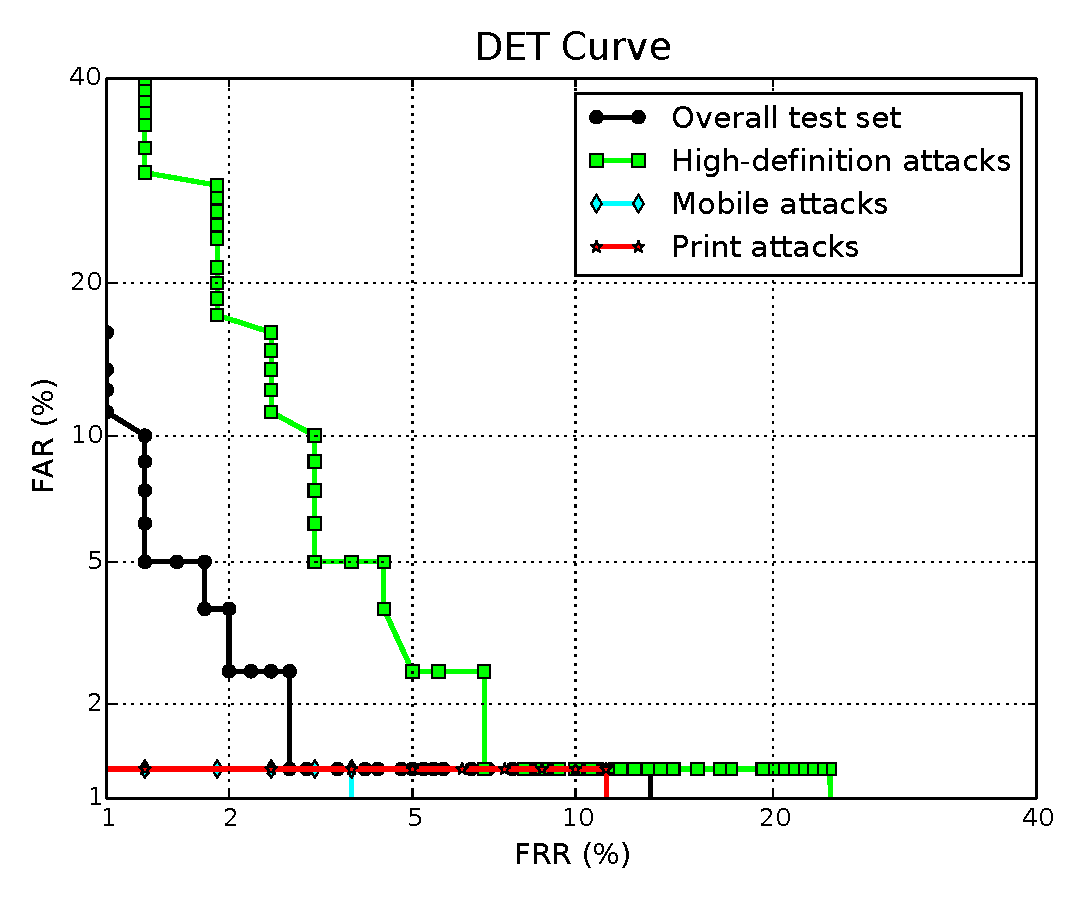
\includegraphics[width=0.45\linewidth]{det_plot_replay_attacks.pdf}}
\subfloat[]{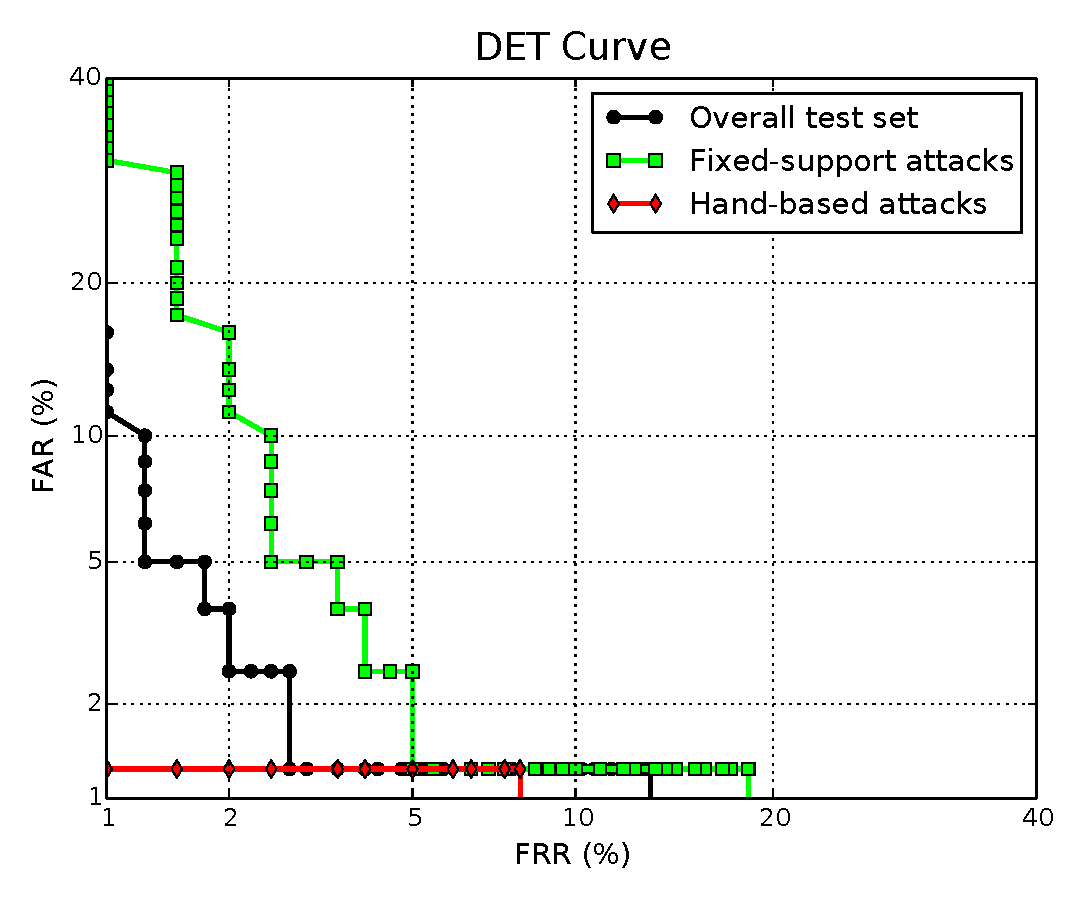
\includegraphics[width=0.45\linewidth]{det_plot_replay_hand_fixed.pdf}}
\caption{{Results obtained on Replay-Attack dataset for each type of attack using fixed-support (a) in contrast with hand-based attacks (b).}}
\label{fig:det_plot_replay_attack}
\end{figure}


\subsubsection{CASIA Face Anti-Spoofing Dataset}\label{subsec:casia_results}
In this experiment, we evaluate the proposed method using the Protocol II (c.f., Sec.~\ref{subsec:Protocol}) and CASIA dataset. 

Table~\ref{table:our_reults_casia} shows the results obtained for the seven {scenarios} of attacks available in this dataset. Fig.~\ref{fig:det_plot_casia}(a) shows that video-based and warp-photo spoofing attacks are easier to be detected by the proposed method (HTER of $ \approx 8\%$). On the other hand, the cut-based spoofing attacks are more difficult to be detected (HTER of $22.22\%$). \redmark{One possible reason for cut-based attacks to be more difficult for detecting is that during an attempted attack based on cut-photos, the photographs are practically in the same position during all the time, generating fewer artifacts along time, whereas for the attempted attacks based on warped-photos, the photographs are bent during the attack to simulate facial motion. In addition, we believe that video-based attacks were easier to be detected because of the inevitable downsize of the high-resolution samples by the screen device used during attack, as also reported by CASIA's authors~\cite{Zhang:ICB:2012}. In this case, many evidences of attempted attacks are generated and added to the fake sample.} 

As for the quality of the acquisition (Fig.~\ref{fig:det_plot_casia}(b)), the proposed method showed better results for attacks carried out with low-quality videos. An interesting result is the best performance of the method to deal with high-resolution videos than normal quality videos. \redmark{We believe that any conclusion would be precipitous because many factors can influence the noise level of a sensor such as sensor imperfections (e.g., appearance of hot pixels, dead pixels, as well as pixel traps under different acquisition conditions). Several works in the literature have explored these issues. For instance, thermal action has a considerable impact over pattern noise of a digital camera and appearance of defective pixels~\cite{Chen2007,Lukas:TIFS:2006,Rocha:2011:VUC}. As we do not assure that the captures/recaptures happened under similar acquisition conditions, it is wiser only to point out the existence of classification differences in this case.}
%
\begin{table}[!htb]
\centering
%\linethickness{1.5mm}
\caption{Performance results for the CASIA dataset.}
\label{table:our_reults_casia}
\begin{tabular}{lcccc}
\topline
\headcol \multicolumn{1}{c}{Dataset} & FAR	& FRR 	& HTER 	& AUC	\\
\midline
		Low quality		  & $10.00$ & $10.00$ & $10.00$ & $98.11$ \\
\rowcol Normal quality    & $17.78$ & $20.00$ & $18.89$ & $87.67$ \\
		High quality 	  & $13.33$ & $13.33$ & $13.33$ & $95.04$ \\
\rowcol Warp photo attack & $7.78$  &  $8.89$ &  $8.33$ & $96.05$ \\
		Cut photo attack  & $22.22$ & $22.22$ & $22.22$ & $87.27$ \\
\rowcol Video attack 	  &  $8.89$ &  $8.89$ &  $8.89$ & $96.41$ \\
\textbf{Overall Attack}   & $\mathbf{14.07}$ &  $\mathbf{14.44}$ &  $\mathbf{14.26}$ & $\mathbf{93.25}$ \\
\bottomline
\end{tabular}
\end{table}
%
\begin{figure}
\centering
\subfloat[]{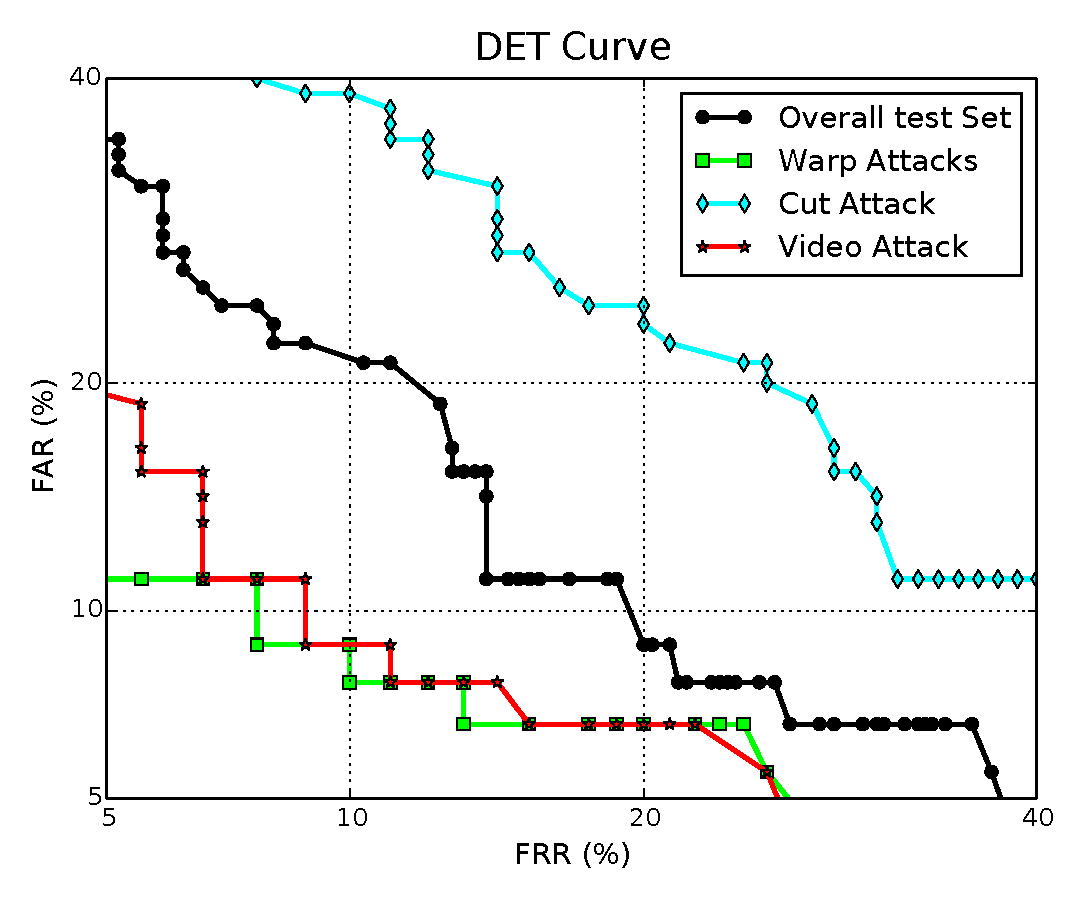
\includegraphics[width=0.45\linewidth]{det_plot_casia_type_attacks.pdf}}
\subfloat[]{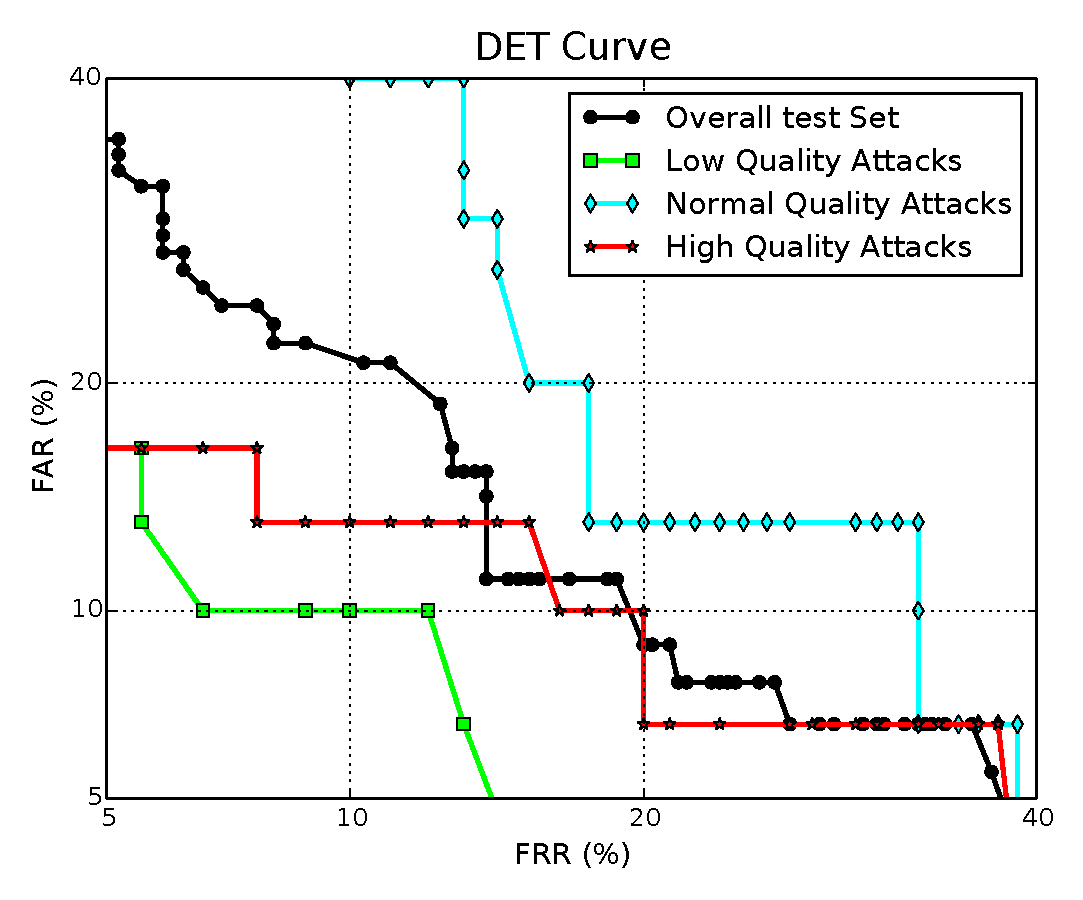
\includegraphics[width=0.45\linewidth]{det_plot_casia_qualy.pdf}}
\caption{Results obtained on CASIA dataset for the three type of attacks (a) and for the three quality of attack (b).}
\label{fig:det_plot_casia}
\end{figure}


\subsubsection{3DMAD Dataset}\label{subsec:3dmad_results}
We now turn our attention \minor{to evaluate} the proposed method for mask-based spoofing attack detection {using the Protocol IV (c.f., Sec.~\ref{subsec:Protocol})}. Using the official \minor{dataset protocol}, the proposed method obtained an AUC of $96.16\%$ and an HTER of $8.0\%$.

\minor{Erdogmus et al.~\cite{Erdogmus:BTAS:2013} reported an HTER of $0.95\%$ using block-based LBP features (local features) and the Linear Discriminant Analysis (LDA) classifier. This performance difference is somewhat explained due to the different validation protocol used. Erdogmus et al. used an $1000$-fold cross validation method and, in each fold, the clients from the dataset were randomly assigned into training, development and test sets. In our case, we randomly divided the clients from dataset and assigned them into training, development and test set only once. Even so, the proposed method outperforms other techniques using global LBP, whose HTERs reported by Erdogmus et al. were all above $10.0\%$.}


\subsubsection{UVAD Dataset}\label{subsec:uvad_results}
In this experiment, we evaluate the proposed method using the Protocol III (c.f., Sec.~\ref{subsec:Protocol}) and UVAD dataset. We also evaluate the proposed method considering LBP-based and motion-based countermeasure methods. 

According to Pereira et al.~\cite{Pereira:ICB:2013}, the correlation method presents an HTER of $11.79\%$ on Replay-Attack. {In turn,} LBP$_{8,1}^{u2}$~\cite{Chingovska:BIOSEG:2012} was effective to characterize the artifacts embedded in the attack videos on Replay-Attack obtaining an HTER of $15.16\%$. In the UVAD dataset, however, both methods obtained a more modest performance as Table~\ref{tab:antispoofing_uvad} shows. With respect to LBP$_{8,1}^{u2}$ method, for instance, the proposed method reduces the classification error in about $36\%$.
%
\begin{table}[!ht]
	\centering
	\caption{Comparison among LBP-based approach~\cite{Chingovska:BIOSEG:2012}, motion-based approach~\cite{Anjos:IJCB:2011} and the proposed method on the UVAD dataset.}
	\label{tab:antispoofing_uvad}
	\begin{tabular}{cccc}
		\topline
		\headcol \textbf{Methods}                         & \textbf{FAR (\%)} & \textbf{FRR (\%)} & \textbf{HTER (\%)} \\ 
		\midline
		Correlation~\cite{Anjos:IJCB:2011}				  & $81.60$ & $14.56$ & $48.06$ \\
		\rowcol LBP$_{8,1}^{u2}$~\cite{Chingovska:BIOSEG:2012}    & $27.41$ & $66.04$ & $46.72$ \\
		\textbf{Proposed Method} & $\mathbf{44.73}$ & $\mathbf{15.00}$ & $\mathbf{29.87}$ \\
		\bottomline		
	\end{tabular}
\end{table}


%Note that our method was trained with the Replay-Attack dataset and tested with 3DMAD dataset, while the method proposed by Erdogmus~\cite{Erdogmus:BTAS:2013} was trained and tested with samples of the same dataset. Even in with the differences existing between the Replay-Attack and 3DMAD dataset (e.g., acquisition sensor, type of attack performed) in this cross-dataset validation protocol, achieved optimal results, which is a remarkable achievement for spoofing detection research.
%%
%\begin{table}[!htb]
%\centering
%%\linethickness{1.5mm}
%\caption{Results (HTER) obtained with our method and with the one proposed method by Erdogmus et al.~\cite{Erdogmus:BTAS:2013} using the 3DMAD dataset.}
%\label{table:3dmad_result}
%\begin{tabular}{lr}
%\toprule
%\multicolumn{1}{c}{Methods} & HTER (\%) \\
%\toprule
% Erdogmus et al.~\cite{Erdogmus:BTAS:2013} & $0.95$ \\
% Proposed Method &  $8.00$ \\
%\bottomrule
%\end{tabular}
%\end{table}

\subsubsection{Comparison with State-of-the-Art Methods for CASIA and Replay-Attack Datasets}

In this section, we compare the proposed method with others \minor{available} in the literature for Replay-Attack and CASIA datasets. Table~\ref{table:CSA} shows results for the Replay-Attack Dataset. The proposed method outperforms the ones based on texture analysis~\cite{Chingovska:BIOSEG:2012,Maatta:IJCB:2011,Pereira:JIVP:2014} and also methods based on motion analysis~\cite{Anjos:IJCB:2011}. It was also more effective than methods based on fusion schemes reported by Pereira et al.~\cite{Pereira:ICB:2013} and Komulainen et al.~\cite{Komulainen:ICB:2013}, with a relative error reduction (RER) of \allan{$67.69\%$ and $46.18\%$}, respectively.
%
\begin{table}[!htb]
\centering
%\linethickness{1.5mm}
\caption{Comparison among the existing methods. The first column shows the HTERs reported by the authors, whereas the second column shows the Relative Error Reduction (RER) obtained with the proposed method. The reported HTERs were obtained using the original Replay-Attack Dataset~\cite{Chingovska:BIOSEG:2012} protocol. \allan{The results highlighted with~$\dagger$~and~$\ddagger$~were reported by Chingovska et al.~\cite{Chingovska:BIOSEG:2012} and Pereira et al.~\cite{Pereira:ICB:2013}, respectively.}}
\label{table:CSA}
\begin{tabular}{lcc}
\topline
\headcol \multicolumn{1}{c}{Methods} & HTER (\%) & RER (\%) \\
\midline
 Chingovska et al.~\cite{Chingovska:BIOSEG:2012} & {15.16} & \allan{81.86} \\
 \rowcol Pinto et al.~\cite{Pinto:TIFS:2015} & 14.27 & \allan{80.73} \\
 \allan{M\"{a}\"{a}tt\"{a} et al.}~\cite{Maatta:IJCB:2011} & 13.87$^\dagger$ & \allan{80.17} \\
 \rowcol \allan{Anjos and Marcel}~\cite{Anjos:IJCB:2011} & 11.79$^{\ddagger}$ & \allan{76.68} \\
 Pereira et al.~\cite{Pereira:ICB:2013} & 8.51 & \allan{67.69} \\
 \rowcol Pereira et al.~\cite{Pereira:JIVP:2014} & 7.60 & \allan{63.82} \\
 Komulainen et al.~\cite{Komulainen:ICB:2013} & 5.11 & \allan{46.18} \\
 \rowcol \textbf{Proposed Method} &  \textbf{2.75} & 0 \\
\bottomlinec
\end{tabular}
\end{table}

Table~\ref{table:soa_casia} shows a comparison among the proposed method and others reported in the literature for CASIA dataset. The proposed method is on par with the best ones in the literature.
%
\begin{table}[!htb]
\centering
%\linethickness{1.5mm}
\caption{Comparison among the proposed method and others available in the literature. According to the authors of the proposed methods, EERs reported were obtained using the original CASIA Dataset~\cite{Zhang:ICB:2012} protocol.}
\label{table:soa_casia}
\begin{tabular}{lr}
\topline
\headcol \multicolumn{1}{c}{Methods} & EER (\%) \\
\midline
 DoG Baseline.~\cite{Zhang:ICB:2012} & 17.0 \\
 \rowcol LBP$_{8,1}^{u2}$.~\cite{Pereira:JIVP:2014} & 16.0 \\
 LBP-TOP$_{8,8,8,1,1,1}^{u2}$.~\cite{Pereira:JIVP:2014} & 10.0 \\
 \rowcol \textbf{Proposed Method}  &  \textbf{14.0} \\
\bottomlinec
\end{tabular}
\end{table}
%
%Finally, Table~\ref{table:CC} shows the results obtained with our method and the teams that participated in the 2013 2nd Competition on Counter Measures to 2D Face Spoofing Attacks~\cite{Chingovska:ICB:2013}. In this comparison, the proposed method is more effective than those methods without fusion schemes and even some using fusion. Note that the choice of parameters for validating our method on CASIA dataset was made using the Replay-Attack dataset. This shows the robustness of our proposed method which were not fully optimized for the dataset in question as many approaches in the literature. We opted for this strategy as we believe it is more realistic in a real-world setting.
%%In this competition, the teams to train ours algorithms using the Replay-Attack and to test them using anonymous test that was built with real samples from Replay-Attack. 
%%
%\begin{table}[!htb]
%\scriptsize
%\centering
%%\linethickness{1.5mm}
%\caption{Results in terms of HTER obtained with our method and with the teams that participated in the 2013 2nd Competition on Counter Measures to 2D Face Spoofing Attacks promoted by the International Conference on Biometrics (ICB)~\cite{Chingovska:ICB:2013}.}
%\label{table:CC}
%\begin{tabular}{lccccccc}
%\topline
%\headcol & \multicolumn{3}{c}{Development} & \multicolumn{3}{c}{Test} & \\
%%\cmidrule(l){2-4}
%%\cmidrule(r){4-7}
%\headcol \multicolumn{-1}{c}{Methods} & FAR & FRR & HTER & FAR & FRR & HTER & Fusion\\
%\midline
%CASIA    & 0.00  & 0.00 & 0.00 & 0.00  & 0.00  & 0.00  & $\checkmark$ \\
%\rowcol IGD      & 5.00  & 8.33 & 6.67 & 17.00 & 1.25  & 9.13  & $\checkmark$ \\
%MaskDown & 1.00  & 0.00 & 0.50 & 0.00  & 5.00  & 2.50  & $\checkmark$ \\
%\rowcol LNMIIT   & 0.00  & 0.00 & 0.00 & 0.00  & 0.00  & 0.00  & $\checkmark$ \\
%MUVIS    & 0.00  & 0.00 & 0.00 & 0.00  & 2.50  & 1.25  & $\checkmark$ \\
%\rowcol PRA Lab  & 0.00  & 0.00 & 0.00 & 0.00  & 2.50  & 1.25  & $\checkmark$ \\
%ATVS     & 1.67  & 0.00 & 0.83 & 2.75  & 21.25 & 12.00 &  \\
%\rowcol Unicamp  & 13.00 & 6.67 & 9.83 & 12.50 & 18.75 & 15.62 &  \\
%\textbf{Proposed Method}  & \textbf{5.00} & \textbf{5.00} & \textbf{5.00} & \textbf{2.00} & \textbf{15.00} & \textbf{8.5} \\
%\bottomline
%\end{tabular}
%\end{table}

%Comparing our method with the ones reported in the literature, our approach presents better results than methods based on texture analysis~\cite{Chingovska:BIOSEG:2012,Maatta:IJCB:2011,Pereira:JIVP:2014} and methods based on motion analysis~\cite{Anjos:IJCB:2011}. Moreover, our approach was more effective than methods based on fusion schemes~\cite{Pereira:ICB:2013,Komulainen:ICB:2013}. {The results shown in Table~\ref{table:CC} reinforce the effectiveness of the proposed method when compared to other solutions without fusion schemes.}

%The CASIA  team proposed a feature-level fusion between one texture descriptor and three motion descriptors. The authors use a multi-scale version of the Linear Binary Patterns (LBP) and  the Gunnar Farneback's algorithm~\cite{Bigun:LNCS:2013} for extracting dense optical flows between two frames of three regions of the scene: head, torso, and background. The team LNMIIT proposed a feature-level fusion for texture and motion-based descriptors. The authors used the LBP to extract micro-texture patterns present in the face region and non-rigid motion analysis approach proposed by Yan et al.~\cite{Yan:ICARCV:2012}.

%Even though there are many studies in the literature showing that the combination of texture and motion-based approaches is a suitable strategy for detecting spoofing attacks~\cite{Yan:ICARCV:2012,Chingovska:ICB:2013,Komulainen:ICB:2013}, we must ensure whether the assumptions made by the motion-based methods (e.g., stationary recognition system, static background) makes sense in a real scenario where the system will be implemented. The assumptions required by the motion-based method are not always satisfied in the scenarios wherein the identifications are made in a totally uncontrolled environment as occur with authentication systems implemented in mobile devices. We do not make such assumptions with the proposed method herein. Finally, any fusion method can also take advantage of our method by adding it to their fusion schemes aiming at improving the final decision of the spoofing attack detection system.

\subsubsection{Analysis of the Minimum Detection Time}\label{subsec:n_frames}

\minor{We now analyze the impact of the video length over the method discriminability for CASIA, Replay-Attack and 3DMAD datasets. This experiment evaluates: the minimum number of frames required for the method to operate; and the method stability, in terms of HTER(\%), for the three different datasets.}

Fig.~\ref{fig:n_frames} indicates that HTER values vary only slightly when we change the video length for the three datasets and that the proposed method uses about two seconds to detect an attempted attack, thus not compromising the transparency of the authentication process.
%
\begin{figure}[h]
\centering
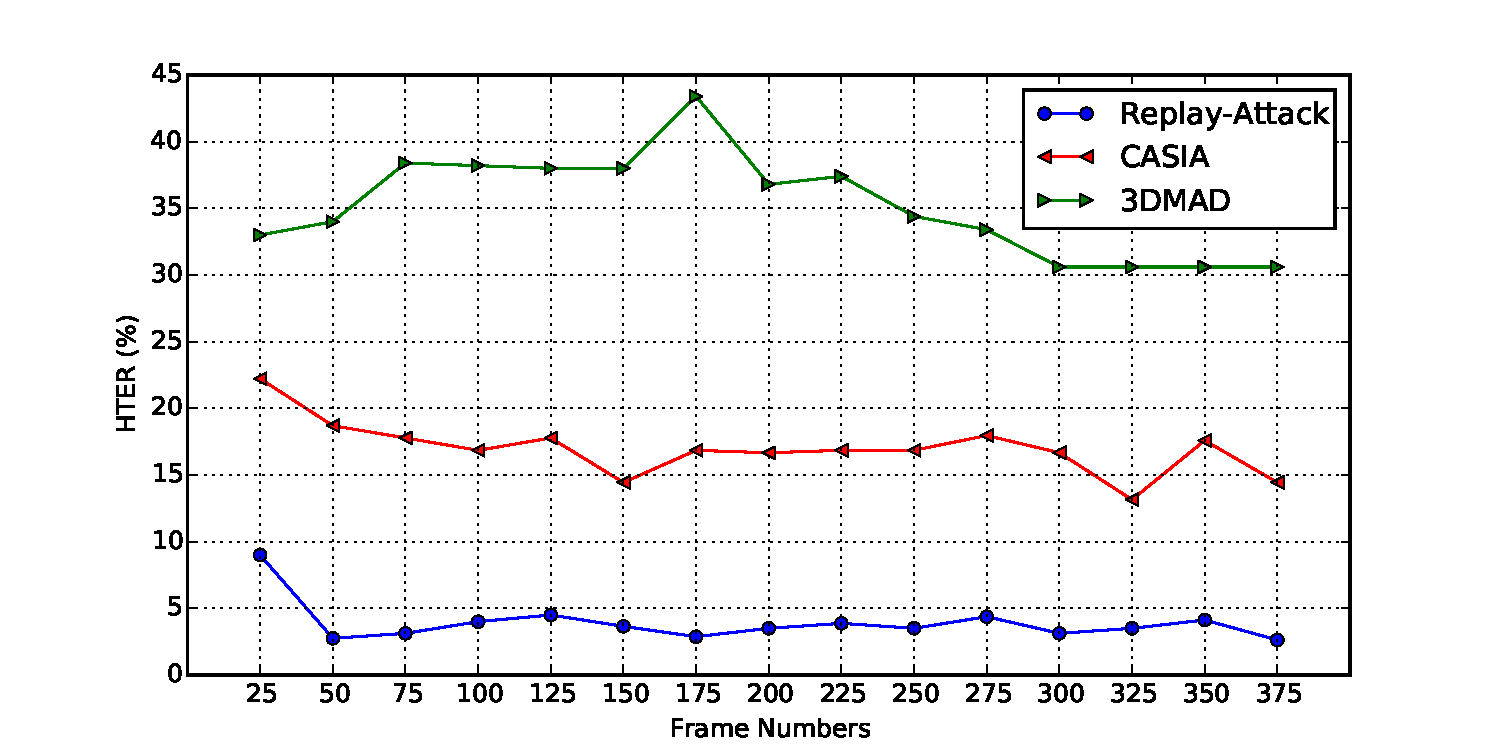
\includegraphics[width=0.45\textwidth]{./figures/n_frames}
\caption{Results in terms of HTER (\%) of the proposed method for different video input length for Replay-Attack, CASIA and 3DMAD datasets.}
\label{fig:n_frames}
\end{figure}

\subsubsection{Cross-Dataset Evaluation}\label{subsec:OtherDatabase}
\minor{In this section, we discuss the performance of the proposed method considering a more difficult scenario (cross-dataset), in which the proposed method is trained with one dataset but it is tested on a different dataset with different acquisition conditions. In this experiment, all datasets used during the training were randomly divided into training and development sets in a proportion of $80\%$ and $20\%$, respectively. The development set is used to estimate the EER threshold that is necessary to calculate the HTER during the test.}

Table~\ref{tab:cross-dataset} shows the results using the cross-dataset protocol. The results indicate that the proposed method presents better generalization when trained with CASIA, with a mean HTER of $40.17\%$. We believe this occurred due to more variability of the type of attacks and video quality in the CASIA dataset, which enriches the training. This dataset contains warped-, cut- and video-based attacks performed with spoofed samples of different quality: low, normal and high quality. Such characteristics enables a better generalization of the method when CASIA is used for training.

{In turn, the best performance when testing the CASIA and 3DMAD datasets was obtained when training with UVAD dataset, another rich dataset for training. Although this dataset contains only video-based spoofing attacks, it has comprises different sensors (for capturing and recapturing the biometric samples) and display devices used during the attempted attacks. We believe that such variability adds different sensor-intrinsic noise levels to the training samples, which contribute to build a more robust classification model.}

{With regard to the more modest generalization presented during the test of the 3DMAD dataset, we believe that it is due to the absence of some artifacts that are commonly found in samples from photo-based and video-based attacks (e.g., blurring, flickering effects) that were not found in the attempted attack video from 3D masks. In addition, spoofing attacks performed with masks are less likely to add temporal disturbances similar to those added when the impostor presents the fake samples, by hand, using a monitor or a photo.}

\minor{Finally, Table~\ref{tab:cross_comparison} shows a comparison among the obtained results reported in the literature. Except for the correlation method, all others present a better performance when they are trained with CASIA. Once again, we believe that our method performs better when training with CASIA because such dataset is more heterogeneous than Replay-Attack. The Correlation~\cite{Anjos:IJCB:2011} and LBP-TOP~\cite{Chingovska:BIOSEG:2012} methods aim to characterize temporal information, similarly to the proposed method, and the results of both methods emphasize the difficulty in characterizing such information completely. In this protocol, besides handling data from different sensors, all methods have to deal with different lighting conditions and background.}

%
%%
%\begin{table}[!htb]
%\scriptsize
%\centering
%%\linethickness{1.5mm}
%\caption{Results in terms of HTER obtained with our method using the cross-dataset Protocol.}
%\label{table:cross}
%\begin{tabular}{lccc}
%\toprule
%\textbf{Datasets} & FAR & FRR & HTER \\
%\toprule
%CASIA  & 11.11 & 83.33 & 47.22 \\
%3DMAD  & 29.41 & 52.94 & 41.18 \\
%UVAD   & 1.34  & {87.17} & {44.26} \\
%\bottomrule
%\end{tabular}
%\end{table}
%
\begin{table*}[!ht]
	\centering
	\footnotesize
	\caption{Results obtained with the cross-dataset protocol and using the overall test sets of each dataset.}
	\label{tab:cross-dataset}	
	\begin{tabular}{cccccc}
		\topline
		\headcol \textbf{Train} & \textbf{Test} & \textbf{FAR (\%)} & \textbf{FRR (\%)} & \textbf{HTER (\%)} & \textbf{Mean HTER (\%)} \\  
		\midline
		%
		& 3DMAD         & 88.00 & 4.00  & 46.00 & \\
		\rowcol 						& Replay-Attack & 32.50 & 36.25 & \textbf{34.38} & \\
		\multirow{-3}{*}{CASIA}         & UVAD          & 38.61 & 41.67 & \textbf{40.14} & \multirow{-3}{*}{ $40.17\%$ } \\
		%
		\hline
		\rowcol									& 3DMAD & 52.00 & 44.00 & 48.00 & \\
		\rowcol									& CASIA & 0.00 & 100.0 & 50.00 & \\
		\rowcol \multirow{-3}{*}{Replay-Attack} & UVAD  & 5.74 & 83.33  & 44.54 & \multirow{-3}{*}{ $47.45\%$ } \\
		%
		\hline
		& 3DMAD         & 84.00 & 4.00  & \textbf{44.00} & \\
		\rowcol							& CASIA         & 13.70 & 63.33 & \textbf{38.52} & \\										
		\multirow{-3}{*}{UVAD}          & Replay-Attack & 79.25 & 6.25 & 42.75  & \multirow{-3}{*}{ $41.76\%$ } \\
		\bottomline 
	\end{tabular} 
\end{table*}
%

%The results show that our method is still not the final word considering a cross-dataset validation (training with one dataset and testing in a different dataset). However, according to other results reported in the literature recently, this behavior is expected, as reported by Pereira et al.~\cite{Pereira:ICB:2013}, whose results in Table~\ref{table:cross_compar} corroborate our findings. We believe that this difficulty of the methods in classifying data from other datasets, not seen during training, is partly because of the different conditions for the acquisition of real samples and recapture of false samples. Therefore, we recommend that either our method is optimized according to the target operational setup or that the method is trained using a good representation of the operational setup of the testing, in other words, the training must comprise examples of situations that could appear during testing. The more complex is the training set the more likely the method will generalize.

%Finally, note that we are not proposing the final word on cross-dataset evaluation. This is a much more challenging problem and here we only touch the tip of the iceberg. Much more work still needs to be done in this direction from all of the research community.
%
%\begin{table}[!htb]
%\scriptsize
%\centering
%%\linethickness{1.5mm}
%\caption{Cross-dataset evaluation comparison of the proposed method with the ones reported in~\cite{Pereira:ICB:2013} for CASIA dataset.}
%\label{table:cross_compar}
%\begin{tabular}{lr}
%\toprule
%\textbf{Datasets} & HTER (\%) \\
%\toprule
%Our method              	 & 47.22   \\
% \hline
%Correlation Motion           & 48.28 \\
%$LBP_{8,1}^{u2}$             & 57.90  \\
%$LBP-TOP_{8,8,8,1,1,1}^{u2}$  & 61.33 \\
%\bottomrule
%\end{tabular}
%\end{table}

%UVAD dataset which contains attempted attacks performed with high quality devices. With this experimental protocol, we obtain an AUC of $94.86\%$ and a HTER of $12.50\%$, considering all attempted attack videos contained on the UVAD dataset. Fig.~\ref{fig:uvad_barplots} shows the results for each sensor acquisition and display devices in the UVAD dataset. The proposed method was capable of capturing noise and artifacts added in the synthetic biometric samples even when the attempted attacks are performed with high quality videos, for different display devices used in the attacks and different biometric sensors. We can conclude that the assumptions made in this work, regarding the perturbations in the frequency components of the signal captured by the acquisition sensor caused by adding noise and artifacts are consistent and generalizable to other attack scenarios.
%%
%\begin{figure*}[!htb]
%\centering
%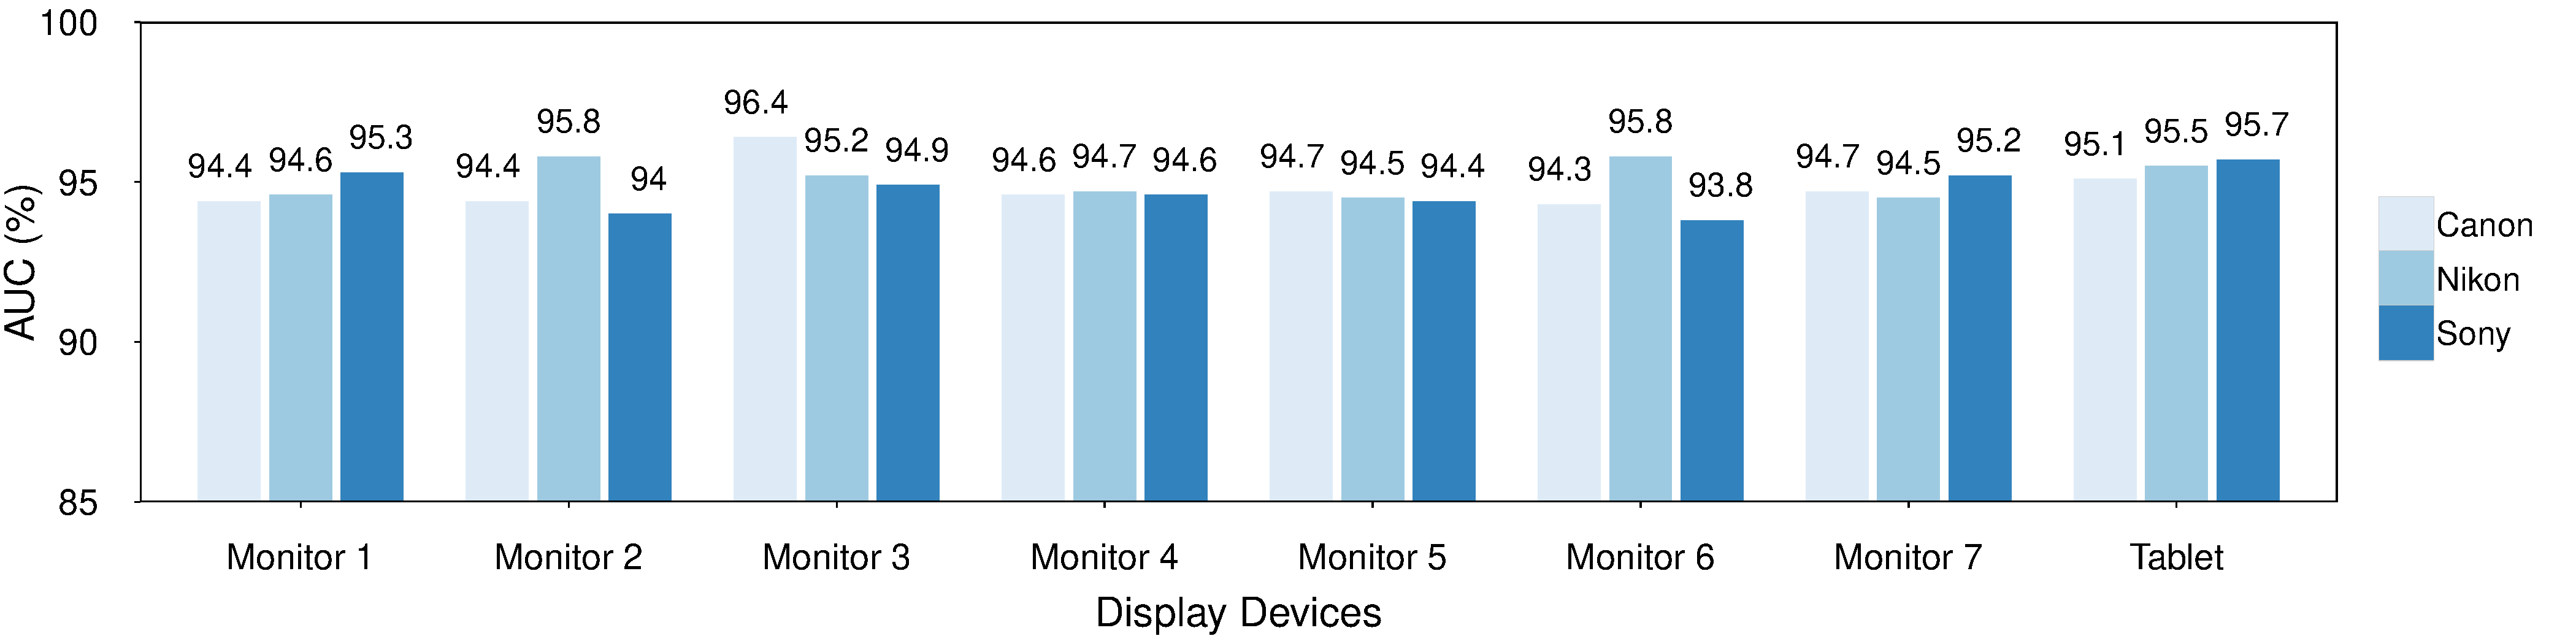
\includegraphics[width=0.99\textwidth]{UVAD_Barplot.pdf}
%\caption{Results (AUC) of the cross-dataset experiment analyzing the different attacks presents on the UVAD dataset. The attacks were performed in three sensor acquisition using eight different display devices.%\newtodo{Remover o fundo cinza.}
%}
%\label{fig:uvad_barplots}
%\end{figure*}

\section{Conclusions and Future Work}\label{sec:conclusions}
In this paper, we proposed an algorithm for detecting spoofing attacks that takes advantage of noise and artifacts added to the synthetic biometric samples during their manufacture and recapture. We showed that the analysis of the behavior of the noise signature, in the frequency domain, is proper to reveal spoofing attacks. For this, we proposed the use of time-spectral features as low-level descriptors, which gather temporal and spectral information in a single feature descriptor. To handle several types of attacks and to obtain a feature descriptor with a suitable generalization, we also proposed the use of the visual codebook concept to find a mid-level representation from time-spectral descriptors. 

The experimental results showed \redmark{that the magnitude is an important characteristic} from a signal, in frequency domain, for spoofing attack detection. We also showed how to use the visual codebook concept effectively in order to find a more robust space representation to the different kinds of attacks and with a good generalization. The obtained results \minor{demonstrated} the effectiveness of the proposed method in detecting different types of attacks (photo-, video-, and 3D-mask-based ones).

\minor{We believe that the frequency-based approach used is effective because we have a decrease in low frequency components due to information loss caused during manufacture of the fake samples (e.g., information loss during printing) and recapture (e.g., blurring effect) and an increase in some high frequency components in the fake samples during recapture due to some artifacts added to the fake samples (e.g., printing artifacts, banding effect, noise added by the imaging sensor). Moreover, these disturbances in the composition of the components of frequencies are best characterized as we analyze the biometric sample in the frequency domain rather than spatial domain and along time instead of on isolated frames or still images.}

% This table comes here because it was showing before another one in the results section
\begin{table}[!ht]
	\centering
	\caption{Comparison among different anti-spoofing methods considering cross-dataset protocol.}
	\label{tab:cross_comparison}
	\begin{tabular}{m{0.11\textwidth}m{0.1\textwidth}m{0.1\textwidth}m{0.08\textwidth}}
		\topline
		\headcol \textbf{Methods} & \textbf{Train} & \textbf{Test} & \textbf{HTER (\%)} \\ 
		\midline
		\multirow{2}{*}{Proposed Method}
		& Replay-Attack & CASIA & 50.00 \\
		& CASIA & Replay-Attack & 34.38 \\
		\hline
		\rowcol													& Replay-Attack & CASIA & 48.28 \\
		\rowcol \multirow{-2}{*}{Correlation} & CASIA & Replay-Attack & 50.25 \\
		\hline
		\multirow{2}{*}{LBP-TOP$_{8,8,8,1,1,1}^{u2}$} & Replay-Attack & CASIA & 61.33 \\
		& CASIA & Replay-Attack & 50.64 \\		
		\hline 
		\rowcol & Replay-Attack & CASIA & 57.90 \\
		\rowcol \multirow{-2}{*}{LBP$_{8,1}^{u2}$} & CASIA & Replay-Attack & 47.05 \\		
		\bottomlinec
	\end{tabular}
\end{table}


\minor{Regarding the important cross-dataset validation, the performed experiments demonstrated that the proposed method and other approaches available in the literature still have modest generalizations. This is of particular importance for the research community as it shows that the problem is still far from solved and cross-dataset validation must be considered from now on when designing and deploying spoofing detection techniques.}



{As discussed earlier, we observed that different biometric sensors present different properties. Therefore, it is important to train a classifier considering this variability. UVAD dataset comes in hand for this purpose and will surely serve the community in this regard with more than 15k samples of hundreds of clients and diverse sensors.}

\minor{Finally, it is worth mentioning that we do not claim to introduce the best method out there for spoofing detection. On the contrary, our very objective in this paper was to show that capturing spatio, spectral and temporal features from biometric samples can be successfully considered in the spoofing detection scenario. That being said, it is likely that the proposed approach, when combined with existing ones in the literature, may as well boost the performance since they will likely rely on complementary features for solving the problem.} 

Directions for future research include the investigation of new approaches to transforming low-level descriptors into mid-level descriptors as Fisher vectors~\cite{Perronnin:ECCV:2010} and Bossa Nova~\cite{Avila:ICIP:2011}. These strategies for finding mid-level representations could also be exploited by methods that use texture-based descriptors. In such cases, the goal would be to investigate whether the representation space found by the texture descriptors used in the literature for detecting face spoofing attacks (e.g., LBP, LBP-TOP, and their variants) could be transformed in a new representation space better adapted to the face spoofing problem in a scenario with different types of attacks.

%\appendices

\section{Convolutional Network Operations}
\label{sec:convnet_ops}

Our networks use classic convolutional operations that can be viewed as linear and non-linear image processing operations. When stacked, these operations essentially extract higher level representations, named \emph{multiband images}, whose pixel attributes are concatenated into high-dimensional feature vectors for later pattern recognition.\footnote{This appendix describes convolutional networks from an image processing perspective, therefore the use of terms like image \emph{domain}, image \emph{band}, \emph{etc.}}

Assuming $\hat{I}=(D_I,\vec{I})$ as a multiband image, where $D_I \subset Z^2$ is the image domain and $\vec{I}(p)=\{I_1(p),I_2(p),\ldots, I_m(p)\}$ is the attribute vector of a $m$-band pixel $p=(x_p,y_p)\in D_I$, the aforementioned operations can be described as follows.

\subsubsection{Filter Bank Convolution}

Let ${\cal A}(p)$ be a squared region centered at $p$ of size $L_{\cal A} \times L_{\cal A}$, such that ${\cal A} \subset D_I$ and $q\in {\cal A}(p)$ iff $\max(|x_q-x_p|,|y_q-y_p|)\leq (L_{\cal A}-1)/2$.
Additionally, let $\Phi=({\cal A},W)$ be a filter with weights $W(q)$ associated with pixels $q\in {\cal A}(p)$.
In the case of multiband filters, filter weights can be represented as vectors $\vec{W}_i(q)=\{w_{i,1}(q),w_{i,2}(q),\ldots,w_{i,m}(q)\}$ for each filter $i$ of the bank, and a multiband filter bank $\Phi = \{\Phi_1, \Phi_2, \ldots, \Phi_n\}$ is a set of filters $\Phi_i=({\cal A},\vec{W}_i)$, $i=\{1,2,\ldots,n\}$.

The convolution between an input image $\hat{I}$ and a filter $\Phi_i$ produces a band $i$ of the filtered image $\hat{J}=(D_J,\vec{J})$, where $D_J \subset D_I$ and $\vec{J}=(J_1,J_2,\ldots,J_n)$, such that for each $p\in D_J$,
\begin{equation}
J_i(p) = \sum_{\forall q\in {\cal A}(p)} \vec{I}(q)\cdot \vec{W}_i(q).
\end{equation}

\subsubsection{Rectified Linear Activation}

Filter activation in this work is performed by rectified linear units (RELUs) of the type present in many state-of-the-art convolutional architectures~\cite{Krizhevsky:2012,Pinto:2011b} and is defined as
\begin{equation}
J_i(p) = \max(J_i(p),0).
\end{equation}

\subsubsection{Spatial Pooling}

Spatial pooling is an operation of paramount importance in the literature of convolutional networks~\cite{LeCun:1998} that aims at bringing translational invariance to the features by aggregating activations from the same filter in a given region. 

Let ${\cal B}(p)$ be a pooling region of size $L_{\cal B} \times L_{\cal B}$ centered at pixel $p$ and $D_K = D_J/s$ be a regular subsampling of every $s$ pixels $p \in D_J$. We call $s$ the \emph{stride} of the pooling operation. Given that $D_J \subset Z^2$, if $s=2$, $|D_K| = |D_J|/4$, for example.
The pooling operation resulting in the image $\hat{K}=(D_K,\vec{K})$  is defined as 
\begin{equation}
K_i(p) = \sqrt[\alpha]{\sum_{\forall q\in {\cal B}(p)} J_i(q)^{\alpha}}, 
\end{equation}
where $p\in D_K$ are pixels in the new image, $i=\{1,2,\ldots,n\}$ are the image bands, and $\alpha$ is a hyperparameter that controls the sensitivity of the operation. In other words, our pooling operation is the $L_{\alpha}$-norm of values in ${\cal B}(p)$. 
The stride $s$ and the size of the pooling neighborhood defined by $L_{\cal B}$ are other hyperparameters of the operation.

\subsubsection{Divisive Normalization}

The last operation considered in this work is divisive normalization, a mechanism widely used in top-performing convolutional networks~\cite{Krizhevsky:2012,Pinto:2011b} that is based on gain control mechanisms found in cortical neurons~\cite{Geisler:1992}.

This operation is also defined within a squared region ${\cal C}(p)$ of size $L_{\cal C} \times L_{\cal C}$ centered at pixel $p$ such that 
\begin{equation}
O_i(p) = \frac{K_i(p)}{\sqrt{\sum_{j=1}^{n}\sum_{\forall q\in {\cal C}(p)} K_j(q)^2}}
\end{equation}
for each pixel $p\in D_O \subset D_K$ of the resulting image $\hat{O}=(D_O,\vec{O})$. Divisive normalization promotes competition among pooled filter bands such that high responses will prevail even more over low ones, further strengthening the robustness of the output representation $\vec{O}$.

\section*{Acknowledgments}
We thank CAPES (DeepEyes Project), FAPESP (\#2010/05647-4), CNPq (\#307113/2012-4, \#304352/2012-8, \#477662/2013-7, \#487529/2013-8 and \#477457/2013-4), FAPEMIG (APQ-01806-13 and APQ-00567-14), and Microsoft Research for the financial support.


% An example of a floating figure using the graphicx package.
% Note that \label must occur AFTER (or within) \caption.
% For figures, \caption should occur after the \includegraphics.
% Note that IEEEtran v1.7 and later has special internal code that
% is designed to preserve the operation of \label within \caption
% even when the captionsoff option is in effect. However, because
% of issues like this, it may be the safest practice to put all your
% \label just after \caption rather than within \caption{}.
%
% Reminder: the "draftcls" or "draftclsnofoot", not "draft", class
% option should be used if it is desired that the figures are to be
% displayed while in draft mode.
%
%\begin{figure}[!t]
%\centering
%\includegraphics[width=2.5in]{myfigure}
% where an .eps filename suffix will be assumed under latex, 
% and a .pdf suffix will be assumed for pdflatex; or what has been declared
% via \DeclareGraphicsExtensions.
%\caption{Simulation Results.}
%\label{fig_sim}
%\end{figure}

% Note that IEEE typically puts floats only at the top, even when this
% results in a large percentage of a column being occupied by floats.


% An example of a double column floating figure using two subfigures.
% (The subfig.sty package must be loaded for this to work.)
% The subfigure \label commands are set within each subfloat command,
% and the \label for the overall figure must come after \caption.
% \hfil is used as a separator to get equal spacing.
% Watch out that the combined width of all the subfigures on a 
% line do not exceed the text width or a line break will occur.
%
%\begin{figure*}[!t]
%\centering
%\subfloat[Case I]{\includegraphics[width=2.5in]{box}%
%\label{fig_first_case}}
%\hfil
%\subfloat[Case II]{\includegraphics[width=2.5in]{box}%
%\label{fig_second_case}}
%\caption{Simulation results.}
%\label{fig_sim}
%\end{figure*}
%
% Note that often IEEE papers with subfigures do not employ subfigure
% captions (using the optional argument to \subfloat[]), but instead will
% reference/describe all of them (a), (b), etc., within the main caption.


% An example of a floating table. Note that, for IEEE style tables, the 
% \caption command should come BEFORE the table. Table text will default to
% \footnotesize as IEEE normally uses this smaller font for tables.
% The \label must come after \caption as always.
%
%\begin{table}[!t]
%% increase table row spacing, adjust to taste
%\renewcommand{\arraystretch}{1.3}
% if using array.sty, it might be a good idea to tweak the value of
% \extrarowheight as needed to properly center the text within the cells
%\caption{An Example of a Table}
%\label{table_example}
%\centering
%% Some packages, such as MDW tools, offer better commands for making tables
%% than the plain LaTeX2e tabular which is used here.
%\begin{tabular}{|c||c|}
%\hline
%One & Two\\
%\hline
%Three & Four\\
%\hline
%\end{tabular}
%\end{table}


% Note that IEEE does not put floats in the very first column - or typically
% anywhere on the first page for that matter. Also, in-text middle ("here")
% positioning is not used. Most IEEE journals use top floats exclusively.
% Note that, LaTeX2e, unlike IEEE journals, places footnotes above bottom
% floats. This can be corrected via the \fnbelowfloat command of the
% stfloats package.


% if have a single appendix:
%\appendix[Proof of the Zonklar Equations]
% or
%\appendix  % for no appendix heading
% do not use \section anymore after \appendix, only \section*
% is possibly needed

% use appendices with more than one appendix
% then use \section to start each appendix
% you must declare a \section before using any
% \subsection or using \label (\appendices by itself
% starts a section numbered zero.)
%


% Can use something like this to put references on a page
% by themselves when using endfloat and the captionsoff option.
\ifCLASSOPTIONcaptionsoff
  \newpage
\fi



% trigger a \newpage just before the given reference
% number - used to balance the columns on the last page
% adjust value as needed - may need to be readjusted if
% the document is modified later
%\IEEEtriggeratref{8}
% The "triggered" command can be changed if desired:
%\IEEEtriggercmd{\enlargethispage{-5in}}

% references section

% can use a bibliography generated by BibTeX as a .bbl file
% BibTeX documentation can be easily obtained at:
% http://www.ctan.org/tex-archive/biblio/bibtex/contrib/doc/
% The IEEEtran BibTeX style support page is at:
% http://www.michaelshell.org/tex/ieeetran/bibtex/
\bibliographystyle{bib/IEEEtran}
\bibliography{references}

% biography section
% 
% If you have an EPS/PDF photo (graphicx package needed) extra braces are
% needed around the contents of the optional argument to biography to prevent
% the LaTeX parser from getting confused when it sees the complicated
% \includegraphics command within an optional argument. (You could create
% your own custom macro containing the \includegraphics command to make things
% simpler here.)
%\begin{IEEEbiography}[{\includegraphics[width=1in,height=1.25in,clip,keepaspectratio]{mshell}}]{Michael Shell}
% or if you just want to reserve a space for a photo:

%\begin{IEEEbiography}{Michael Shell}
%Biography text here.
%\end{IEEEbiography}
%
%% if you will not have a photo at all:
%\begin{IEEEbiographynophoto}{John Doe}
%Biography text here.
%\end{IEEEbiographynophoto}

% insert where needed to balance the two columns on the last page with
% biographies
%\newpage

%\begin{IEEEbiographynophoto}{Jane Doe}
%Biography text here.
%\end{IEEEbiographynophoto}

% You can push biographies down or up by placing
% a \vfill before or after them. The appropriate
% use of \vfill depends on what kind of text is
% on the last page and whether or not the columns
% are being equalized.

%\vfill

% Can be used to pull up biographies so that the bottom of the last one
% is flush with the other column.
%\enlargethispage{-5in}



% that's all folks
\end{document}


